% Compile with XeLaTeX or LuaLaTeX
\documentclass[10pt]{article}  % Spivak uses ~10pt

% -----------------------------
% Fonts
% -----------------------------
\usepackage{fontspec}
\setmainfont{TeX Gyre Pagella}
\usepackage{unicode-math}
\setmathfont{Libertinus Math}

% -----------------------------
% Page layout
% -----------------------------
\usepackage[margin=2.5cm]{geometry}
\usepackage[parfill]{parskip}

% -----------------------------
% Theorems and QED
% -----------------------------
\usepackage{amsthm}
\usepackage{textcomp}
\usepackage{tcolorbox}
\tcbuselibrary{breakable}

% QED symbol like Spivak (tall gray rectangle)
\renewcommand{\qedsymbol}{\textcolor{black}{\rule{1ex}{2.2ex}}}

\newtheorem{theorem}{Theorem}
\newtheorem{axiom}{Axiom}
\newtheorem{definition}{Definition}

% -----------------------------
% Misc packages
% -----------------------------
\usepackage{graphicx, subfig}
\usepackage{booktabs, array}
\usepackage{paralist, verbatim}
\usepackage{xcolor, pagecolor}
\usepackage{fancyhdr}
\pagestyle{fancy}
\renewcommand{\headrulewidth}{0pt}
\lhead{}\chead{}\rhead{}
\lfoot{}\cfoot{\thepage}\rfoot{}
\usepackage{sectsty}
\allsectionsfont{\sffamily\mdseries\upshape}
\usepackage[nottoc,notlof,notlot]{tocbibind}
\usepackage[titles,subfigure]{tocloft}
\renewcommand{\cftsecfont}{\rmfamily\mdseries\upshape}
\renewcommand{\cftsecpagefont}{\rmfamily\mdseries\upshape}
\usepackage{changepage, comment}
\usepackage{tikz}
\usepackage{pgfplots}
\pgfplotsset{compat=1.18}
% Define a light gray
\definecolor{lightgraypaper}{RGB}{240,240,240}
% Set the page background
\pagecolor{lightgraypaper}
\color{black} % keep text black

\title{Basic Mathematics by Lang}
\author{Noah Lewis}
\begin{document}
\maketitle

\tableofcontents

\section{Numbers}
\subsection{Polynomials and Affine Space}

\begin{tcolorbox}[title=Problem 2, breakable]
    Let $\mathcal{F}_2$ be the field from Exercise 1.
    \begin{enumerate}
        \item Consider the polynomial $g(x, y) = x^2 y + y^2 x \in \mathcal{F}_2[x, y]$.
        Show that $g(x, y) = 0s$ for every $(x, y) \in \mathcal{F}_2^2$, and explain why this 
        does not contradict Proposition 5.
        \item Find a nonzero polynomial in $\mathcal{F}_2[x, y, z]$ which vanishes at every point of $\mathcal{F}_2^3$.
        Try to find one involving three variables.
        \item Find a nonzero polynomial in $\mathcal{F}_2[x_1, \ldots, x_n]$ which vanishes at every point of $\mathcal{F}_2^n$.
                Can you find one in which all of $x_1, \ldots, x_n$ appear?
    \end{enumerate}
\end{tcolorbox}

\textbf{Solution (1):}
It is clear that if $x = 0$ or $y = 0$, then $g(x, y) = 0$.
Now, if $x = y = 1$, then
\[
g(x, y) = 1^2 \cdot 1 + 1^2 \cdot 1 = 1 + 1 = 0.
\]
Thus $g(x, y) = 0$ for all $(x, y) \in \mathcal{F}_2^2$.

\textbf{Solution (2):}
Consider the polynomial $g \in \mathcal{F}_2[x, y, z]$ defined by
\[
g(x, y, z) = (x^2 - x)(y^2 - y)(z^2 - z),
\]
which is clearly $0$ at all $(x, y, z) \in \mathcal{F}_2 \times \mathcal{F}_2 \times \mathcal{F}_2$.

\textbf{Solution (3):}
Consider the polynomial $g \in \mathcal{F}_2[x_1, \ldots, x_n]$ defined by
\[
g(x_1, \ldots, x_n) = (x_1^2 - x_1)\cdots(x_n^2 - x_n),
\]
which is clearly $0$ at all $(x_1, \ldots, x_n) \in \mathcal{F}_2 \times \cdots \times \mathcal{F}_2$.


\begin{tcolorbox}[title=Problem 3, breakable]
    (Requires abstract algebra)
    Let $p$ be a prime number.
    The ring of integers modulo $p$ is a field with $p$ elements, which we will denote $\mathcal{F}_p$.
    \begin{enumerate}
        \item Explain why $\mathcal{F}_p \setminus \{0\}$ is a group under multiplication.
        \item Use Lagrange's theorem to show that $a^{p - 1} = 1$ for all $a \in \mathcal{P} \setminus \{0\}$.
        \item Prove that $a^p = a$ for all $a \in \mathcal{F}_p$. [Hint: Treat the cases $a = 0$ and $a \ne 0$ separately.]
        \item Find a nonzero polynomial in $\mathcal{F}_p[x]$ that vanishes at all points in $\mathcal{F}_p$. [Hint: Use part (c).]
    \end{enumerate}
\end{tcolorbox}

\textbf{Solution (1):}
It is well known that for any ring $R$ the set of units $U(R)$
    under multiplication forms a group.
All elements $x \ne 0$ in $\mathcal{F}_p$ have inverses and are thus in $U(\mathcal{F}_p)$.
Therefore $\mathcal{F}_p \setminus \{0\}$ is a group under multiplication.

\textbf{Solution (2):}
Don't have preqreuisites.

\begin{proof}
    Let $a \in \mathcal{F}_p$.
    Suppose $a = 0$. Then $a^p = 0^p = 0 = a$.
    Suppose $a \ne 0$. Then $a^{p - 1} = 1$ by part 2.
    Then $a \cdot a^{p - 1} = a \cdot 1 \iff a^p = a$ as required.
\end{proof}

\textbf{Solution (4):}
Consider the polynomial $g(x) = x^p - x \in \mathcal{F}_p[x]$.
Now, for all $a \in \mathcal{F}_p$ we have $a^p = a$ by part 3, thus $g(a) = 0$.

\begin{tcolorbox}[title=Problem 5, breakable]
    In the proof of Proposition 5, we took $f \in k[x_1, \ldots, x_n]$ and wrote it as a polynomial
    in $x_n$ with coefficients in $k[x_1, \ldots, x_{n - 1}]$. To see what this looks like in a specific case,
    consider the polynomial
    \[f(x, y, z) = x^5 y^2 z - x^4 y^3 + y^5 + x^2 z - y^3 z + xy + 2x - 5z + 3.\]
    \begin{enumerate}
        \item Write $f$ as a polynomial in $x$ with coefficients in $k[y, z]$.
        \item Write $f$ as a polynomial in $y$ with coefficients in $k[x, z]$.
        \item Write $f$ as a polynomial in $z$ with coefficients in $k[x, y]$.
    \end{enumerate}
\end{tcolorbox}

\textbf{Solution (1):}
\[f(x) =  (y^2 z)x^5 - (y^3) x^4 + (z) x^2 + (y + 2)x - y^3 z + y^5 - 5z + 3\]
\textbf{Solution (2):}
\[f(y) = y^5 - (x^4  - z) y^3 + (x^5 z) y^2  + (x)y + x^2 z + 2x - 5z + 3\]
\textbf{Solution (3):}
\[f(z) = (x^5 y^2  + x^2 - y^3  - 5) z - x^4 y^3 + y^5 + xy + 2x + 3\]


\begin{tcolorbox}[title=Problem 6, breakable]
    Inside of $\mathbb{C}^n$, we have the subset $\mathbb{Z}^n$, which consists of all points with integer coordinates.
    \begin{enumerate}
        \item Prove that if $f \in \mathbb{C}[x_1, \ldots, x_n]$ vanishes at every point of $\mathbb{Z}^n$, then $f$
                is the zero polynomial. [Hint: Adapt the proof of Proposition 5.]
        \item Let $f \in \mathbb{C}[x_1, \ldots, x_n]$, and let $M$ be the largest power of any variable that appears in $f$.
              Let $\mathbb{Z}_{M + 1}^n$ be the set of all points of $\mathbb{Z}^n$, all coordinates which lie between $1$ and $M + 1$, inclusive.
              Prove that if $f$ vanishes at all points of $\mathbb{Z}_{M + 1}^n$, then $f$ is the zero polynomial.
    \end{enumerate}
\end{tcolorbox}

\begin{proof}
    Suppose $f \in \mathbb{C}[x_1, \ldots, x_n]$ vanishes at every point of $\mathbb{Z}^n$.
    We will use induction on the number of variables $n$.
    When $n = 1$. It is well known that a nonzero polynomial in $\mathbb{C}[x]$ of degree $m$
    has at most $m$ distinct roots. For our particular $f \in \mathbb{C}[x]$, we are assuming $f(a) = 0$
    for all $a \in \mathbb{Z}$. Since $\mathbb{Z}$ is infinite, this means that $f$ has infinitely many roots, and, hence,
    $f$ must be the zero polynomial.

    Now assume that the theorem holds for $n - 1$ variables.
    By collecting the various powers of $x_n$, we can write $f$ in the form 
    \[f = \sum_{i = 0}^{N} g_i (x_1, \ldots, x_{n - 1}) x_n^i,\]
    where $g_i \in \mathbb{C}[x_1, \ldots, x_{n - 1}]$. We will show that each $g_i$ 
    is the zero polynomial in $n - 1$ variables, which will force $f$ to be the zero polynomial in $\mathbb{C}[x_1, \ldots, x_n]$.

    If we fix $(a_1, \ldots, a_{n - 1}) \in \mathbb{Z}^{n - 1}$, we get the polynomial 
    $f(a_1, \ldots, a_{n - 1}, x_n) \in \mathbb{C}[x_n]$.
    By our hypothesis on $f$, this vanishes for every $a_n \in \mathbb{Z}$. 
    It follows from the case $n = 1$ that $f(a_1, \ldots, a_{n - 1}, x_n)$ is the zero polynomial in $\mathbb{C}[x_n]$.
    Using the above formula for $f$, we see that all coefficients of $f(a_1, \ldots, a_{n - 1}, x_n)$ vanish.
    Since $(a_1, \ldots, a_{n - 1})$ was arbitrarily chosen in $\mathbb{Z}^{n - 1}$,
    it follows that each $g_i \in \mathbb{C}[x_1, \ldots, x_{n - 1}]$ gives the zero function on $\mathbb{Z}^{n - 1}$. 
    Our inductive assumption then implies each $g_i$ is the zero polynomial in $\mathbb{C}[x_1, \ldots, x_{n - 1}]$.
    This forces $f$ to be the zero polynomial in $\mathbb{C}[x_1, \ldots, x_n]$.
\end{proof}

\begin{proof}
    Suppose $f \in \mathbb{C}[x_1, \ldots, x_n]$ vanishes at every point of $\mathbb{Z}_{M + 1}^n$.
    We will use induction on the number of variables $n$.
    When $n = 1$. It is well known that a nonzero polynomial in $\mathbb{C}[x]$ of degree at most $M$
    has at most $M$ distinct roots. For our particular $f \in \mathbb{C}[x]$, we are assuming $f(a) = 0$
    for all $a \in \mathbb{Z}_{M + 1}$. Since $\mathbb{Z}_{M + 1}$ has $M + 1$ elements, this means that $f$ has $M + 1$ roots, and, hence,
    $f$ must be the zero polynomial.

    Now assume that the theorem holds for $n - 1$ variables.
    By collecting the various powers of $x_n$, we can write $f$ in the form 
    \[f = \sum_{i = 0}^{N} g_i (x_1, \ldots, x_{n - 1}) x_n^i,\]
    where $g_i \in \mathbb{C}[x_1, \ldots, x_{n - 1}]$. We will show that each $g_i$ 
    is the zero polynomial in $n - 1$ variables, which will force $f$ to be the zero polynomial in $\mathbb{C}[x_1, \ldots, x_n]$.

    If we fix $(a_1, \ldots, a_{n - 1}) \in \mathbb{Z}_{M + 1}^{n - 1}$, we get the polynomial 
    $f(a_1, \ldots, a_{n - 1}, x_n) \in \mathbb{C}[x_n]$.
    By our hypothesis on $f$, this vanishes for every $a_n \in \mathbb{Z}_{M + 1}$. 
    It follows from the case $n = 1$ that $f(a_1, \ldots, a_{n - 1}, x_n)$ is the zero polynomial in $\mathbb{C}[x_n]$.
    Using the above formula for $f$, we see that all coefficients of $f(a_1, \ldots, a_{n - 1}, x_n)$ vanish.
    Since $(a_1, \ldots, a_{n - 1})$ was arbitrarily chosen in $\mathbb{Z}_{M + 1}^{n - 1}$,
    it follows that each $g_i \in \mathbb{C}[x_1, \ldots, x_{n - 1}]$ gives the zero function on $\mathbb{Z}_{M + 1}^{n - 1}$. 
    Our inductive assumption then implies each $g_i$ is the zero polynomial in $\mathbb{C}[x_1, \ldots, x_{n - 1}]$.
    This forces $f$ to be the zero polynomial in $\mathbb{C}[x_1, \ldots, x_n]$.
\end{proof}

\subsection{Affine Varieties}

\begin{tcolorbox}[title=Problem 1, breakable]
    Sketch the following affine varieties in $\mathbb{R}^2$:
    \begin{enumerate}
        \item \textbf{V}$(x^2 + 4y^2 + 2x - 16y + 1)$
        \item \textbf{V}$(x^2 - y^2)$
        \item \textbf{V}$(2x + y - 1, 3x - y + 2)$
    \end{enumerate}
    In each case, does the variety have the dimension you would intuitively expect it to have?
\end{tcolorbox}

\textbf{Solution (1):} I would expect it to have two dimensions.
Notice 
\begin{align*}
    x^2 + 4y^2 + 2x - 16y + 1 = 0
    &\iff x^2 + 2x + 1 + 4y^2 - 16y = 0 \\
    &\iff (x + 1)^2 + 4(y^2 - 4y) = 0 \\
    &\iff (x + 1)^2 + 4(y^2 - 4y + 4 - 4) = 0 \\
    &\iff (x + 1)^2 + 4((y - 2)^2 - 4) = 0 \\
    &\iff (x + 1)^2 + 4(y - 2)^2 - 16 = 0  \\
    &\iff \frac{(x + 1)^2}{4} + \frac{(y - 2)^2}{1} = 4
\end{align*}
Which is an ellipse.
\begin{figure}[h!]
    \centering
    \includegraphics[width=0.3\textwidth]{images/chapter1/1.png}
\end{figure}

\textbf{Solution (2):} I would expect it to have two dimensions.
If we solve $x^2 - y^2$ for $y$ we find $y = \pm x$ which is two lines 
with slope of $1$ passing through the origin.
\begin{figure}[h!]
    \centering
    \includegraphics[width=0.3\textwidth]{images/chapter1/2.png}
\end{figure}

\textbf{Solution (3):} I would expect it to be a single point.
We can solve for $x, y$ and find $x = -\frac{1}{5}$, $y = \frac{7}{5}$.
\begin{figure}[h!]
    \centering
    \includegraphics[width=0.3\textwidth]{images/chapter1/3.png}
\end{figure}


\begin{tcolorbox}[title=Problem 6, breakable]
    Let us show that all finite subset of $k^n$ are affine varieties.
    \begin{enumerate}
        \item Prove that a single point $(a_1, \ldots, a_n) \in k^n$ is an affine variety.
        \item Prove that every finite subset of $k^n$ is an affine variety. [Hint: Lemma 2 will be useful.]
    \end{enumerate}
\end{tcolorbox}


\begin{proof}
    Let $(a_1, \ldots, a_n)$ be an arbitrary point in $k^n$.
    Consider the following set of polynomials
    \[\mathcal{P} = \{x_i - a_i \mid 1 \le i \le n\}.\]
    For which the point $(a_1, \ldots, a_n)$ is the exact solution.
    Thus
    \[
        \mathbf{V}(\mathcal{P})
        = \{(a_1, \ldots, a_n)\}.
    \]
    Therefore a single point in $k^n$ is an affine variety.
\end{proof}

\begin{proof}
    Let $V \subset k^n$ be a finite set.
    Then $V$ can be written as
    \[
        V = \bigcup_{i=1}^m \{p_i\},
    \]
    where each $p_i \in k^n$.
    By part (1), each $\{p_i\}$ is an affine variety.
    By Lemma 2, a finite union of affine varieties is an affine variety.
    Thus $V$ is an affine variety.
\end{proof}


\begin{tcolorbox}[title=Problem 8, breakable]
    It can take some work to show that something is \emph{not}
    an affine variety. For example, consider the set 
    \[X = \{(x, x) \mid x \in \mathbb{R}, x \ne 1\} \subseteq \mathbb{R}^2\]
    which is the straight line $x = y$ with the point $(1, 1)$ removed.
    To that $X$ is not an affine variety, suppose that 
    $X = \textbf{V}(f_1, \ldots, f_s)$. Then each $f_i$ vanishes on $X$, and if 
    we can show that $f_i$ also vanishes at $(1, 1)$, we will get the desired contradiction.
    Thus, here is what you are to prove: if $f \in \mathbb{R}[x, y]$ vanishes on $X$,
    then $f(1, 1) = 0$. [Hint: Let $g(t) = f(t, t)$ which is a polynomial $\mathbb{R}[t]$.
    Now apply the proof of proposition 5 on 1.]
\end{tcolorbox}

\begin{proof}
    Suppose $f \in \mathbb{R}[x, y]$ vanishes on $X$.
    Let $g(t) = f(t, t)$, which is a polynomial in $\mathbb{R}[t]$.
    Then $g(x) = 0$ for all $x \in \mathbb{R}$ with $x \ne 1$. 
    Since a nonzero polynomial in $\mathbb{R}[t]$ can have only finitely many roots, 
    it follows from Proposition 5 that $g$ must be the zero polynomial. 
    Therefore $g(1) = f(1, 1) = 0$, which is a contradiction.
\end{proof}

\begin{tcolorbox}[title=Problem 9, breakable]
    Let $\textbf{R} = \{(x, y) \in \mathbb{R}^2 \mid y > 0\}$ be the upper half plane.
    Prove that $\textbf{R}$ is not an affine variety.
\end{tcolorbox}

\begin{proof}
    Suppose $f \in \mathbb{R}[x, y]$ vanishes on $\textbf{R}$.
    Fix any $y_0 > 0$ and consider the polynomial in one variable $g(x) = f(x, y_0) \in \mathbb{R}[x]$.
    Since $f(x, y_0) = 0$ for all $x \in \mathbb{R}$ by Proposition 5, $g$ is the zero polynomial.
    Because $y_0 > 0$ was arbitrary it follows that that $f(x, y) = 0$ for all $(x, y) \in \textbf{R}$.  
    Therefore $f$ is the zero polynomial.
\end{proof}

\begin{tcolorbox}[title=Problem 10, breakable]
    Let $\mathbb{Z}^n \subseteq \mathbb{C}^n$ consist of those points with integer coordinates.
    Prove that $\mathbb{Z}^n$ is not an affine variety. [Hint: See Exercise 6 1.]
\end{tcolorbox}

\begin{proof}
    Suppose $f \in \mathbb{C}[x_1, \dots, x_n]$ vanishes on $\mathbb{Z}^n$.
    Fix integers $k_2, \dots, k_n \in \mathbb{Z}$ and consider the polynomial
    \[
        g(x_1) = f(x_1, k_2, \dots, k_n) \in \mathbb{C}[x_1].
    \]
    Since $g(x_1) = f(x_1, k_2, \dots, k_n) = 0$ for all $x_1 \in \mathbb{Z}$, by Proposition 5 it follows that $g$ is the zero polynomial.
    Because $k_2, \dots, k_n$ were arbitrary integers, it follows that $f(x_1, x_2, \dots, x_n) = 0 \quad \text{for all } (x_1, \dots, x_n) \in \mathbb{Z}^n$.
    Therefore $f$ is the zero polynomial in $\mathbb{C}[x_1, \dots, x_n]$.
\end{proof}


\begin{tcolorbox}[title=Problem 11, breakable]
    So far, we have discussed varieties in $\mathbb{R}$ or $\mathbb{C}$.
    It is also possible to consider varieties over the field $\mathbb{Q}$,
    although the questions here tend to be \emph{much} harder.
    For example, let $n$ be a positive integer, and consider the variety 
    $F_n \subseteq \mathbb{Q}^2$ defined by
    \[x^n + y^n = 1.\]
    Notice that there are some obvious solutions when $x$ or $y$ is zero.
    We call these \emph{trivial solutions}.
    An interesting question is whether or not there are any nontrivial solutions.
    \begin{enumerate}
        \item Show that $F_n$ has two trivial solutions if $n$ is odd and four trivial solutions of $n$ is even.
        \item Show that $F_n$ would have a nontrivial solution for some $n \ge 3$ if and only if Fermat's Last Theorem were false.
    \end{enumerate}
    \begin{theorem}
        \emph{Fermat's Last Theorem} states that, for $n \ge 3$, the equation
        \[x^n + y^n = z^n\]
        has no solutions where $x, y$ and $z$ are nonzero integers.
        The general case of this conjecture was proved by Andrew Wiles in 1994 using some 
        very sophisticated number theory. The proof is \emph{extremely} difficult.
    \end{theorem}
\end{tcolorbox}


\begin{proof}
    Suppose $n$ is odd. 
    If $x = 0$ then $y = 1$.
    Similarly, if $y = 0$ then $x = 1$.
    Thus we have two solutions: $(0, 1), (1, 0)$.

    Suppose $n$ is even.
    If $x = 0$ then $y = \pm 1$.
    Similarly, if $y = 0$ then $x = \pm 1$.
    Thus we have four solutions: $(0, \pm 1), (\pm 1, 0)$.
\end{proof}

\begin{proof}
    Suppose $F_n$ has a nontrivial solution for some $n \ge 3$.
    Then suppose $x, y \in \mathbb{Q}$ such that $x^n + y^n = 1$.
    Furthermore, suppose $x = \frac{a}{b}, y = \frac{c}{d}$ where $a, b, c, d \in \mathbb{Z}$.
    Then 
    \[
        \left(\frac{a}{b}\right)^n + \left(\frac{c}{d}\right)^n = \frac{a^n}{b^n} + \frac{c^n}{d^n} = 1.
    \]
    Multiply through by $b^n d^n$ to obtain 
    \[
        (a d)^n + (c b)^n = (b d)^n.
    \]
    Since $a, b, c, d \in \mathbb{Z}$ and $n \ge 3$, this is a solution to Fermat's Last Theorem.

    Conversely, suppose Fermat's Last Theorem is false.
    Then there exists nonzero integers $x, y, z$ and $n \ge 3$ such that $x^n + y^n = z^n$.
    Dividing through by $z^n$ gives
    \[
        \left(\frac{x}{z}\right)^n + \left(\frac{y}{z}\right)^n = 1.
    \]
    Therefore $F_n$ has a nontrivial solution for some $n \ge 3$.
\end{proof}


\begin{tcolorbox}[title=Problem 15, breakable]
    In Lemma 2, we showed that if $V$ and $W$ are affine varieties,
    then so are there union $V \cup W$ and intersection $V \cap W$.
    In this exercise we will study how other set-theoretic operations 
    affect affine varieties.
    \begin{enumerate}
        \item Prove that finite unions and intersections of affine varieties are again affine varieties. [Hint: Induction].
        \item Give an example to show that an infinite union of affine varieties need not be an affine variety.
              Hint: By Exercise 8-10, we know some subsets of $k^n$ that are not affine varieties.
              Suprisingly, an infinite intersection of affine varieties is still an affine variety.
              This is a consequence of the Hilbert Basis Theorem, which will be discussed in Chapter 2.
        \item Given an example to show that the set-theoretic difference $V \setminus W$ of two affine varieties
              need not be an affine varietiy.
        \item Let $V \subseteq k^n$ and $W \subseteq k^m$ be two affine varieties, and let 
        \[V \times W = \{(x_1, \ldots, x_n, y_1, \ldots, y_m) \in k^{n + m} \mid (x_1, \ldots, x_n) \in V, (y_1, \ldots, y_n) \in W\}\]
        be their Cartesian product. Prove that $V \times W$ is an affine variety in $k^{n + m}$.
        [Hint: If $V$ is defined by $f_1, \ldots, f_s \in k[x_1, \ldots, x_n]$, then we can regard $f_1, \ldots, f_s$
        as polynomials in $k[x_1, \ldots, x_n, y_1, \ldots, y_m]$, and similarly for $W$. Show that this gives defining
        equations for the Cartesian product.]
    \end{enumerate}
\end{tcolorbox}

\begin{proof}
    By Lemma 2 we know the base case holds for the union and intersection of two affine varieties.
    Suppose Lemma 2 holds for the union and intersection of $n - 1$ affine varieties.
    Let $V = \{v_1, \ldots, v_n\}$ be a set of $n$ affine varieties.
    Then 
    \[\mathcal{U} = \bigcup_{i = 1}^{n} v_i = \bigcup_{i = 1}^{n - 1} v_i \cup v_n,\]
    and
    \[\mathcal{I} = \bigcap_{i = 1}^{n} v_i = \bigcap_{i = 1}^{n - 1} v_i \cap v_n.\]
    Now, by our hypothesis $\bigcup_{i = 1}^{n - 1} v_i$ and $\bigcap_{i = 1}^{n - 1} v_i$
        are affine varieties.
    Then by Lemma 2, $\bigcup_{i = 1}^{n - 1} v_i \cup v_n$ and $\bigcap_{i = 1}^{n - 1} v_i \cap v_n$
        are also affine varieties.
    Thus $\mathcal{U}$ and $\mathcal{I}$ are affine varieties.
\end{proof}

\begin{proof}
    Consider the union of all points in $\mathbb{Z}^n$.
    Each point is an affine variety by Problem 6.
    However, by Problem 10, their union (which is $\mathbb{Z}^n$) is not an affine variety.
\end{proof}

\begin{proof}
    Consider the varieties $V_1 = \{(x, y) \mid x = y\}$ and $V_2 = \{(1, 1)\}$.
    By Problem 8, $V_1 \setminus V_2$ is not an affine variety.
\end{proof}

\begin{proof}
    Let $V \subseteq k^n$ be defined by polynomials $f_1, \ldots, f_s \in k[x_1, \ldots, x_n]$
        and $W \subseteq k^m$ be defined by polynomials $g_1, \ldots, g_t \in k[y_1, \ldots, y_m]$.
    Then, let $f_1, \ldots, f_s \in k[x_1, \ldots, x_n, y_1, \ldots, y_m]$
    and $g_1, \ldots, g_t \in k[x_1, \ldots, x_n, y_1, \ldots, y_m]$.
    Then
    \[
        V \times W = \textbf{V}(f_1, \ldots, f_s, g_1, \ldots, g_t) \subseteq k^{n + m},
    \]
    so $V \times W$ is an affine variety.
\end{proof}

\subsection{Parametrizations of Affine Varieties}

\begin{tcolorbox}[title=Problem 1, breakable]
    Parametrize all solutions of the linear equations 
    \[x + 2y - 2z + w = 1,\]
    \[x + y + z - w = 2.\]
\end{tcolorbox}

\begin{proof}
    We use row reduction to find the simplified equations:
    \[
        x - 4z + 3w = 3, \quad
        y - 3z + 2w = -1.
    \]
    Then let $s = w$ and $t = z$.
    Then
    \[
        x = 3 + 4t - 3s, \quad
        y = -1 + 3t - 2s.
    \]
\end{proof}

\begin{tcolorbox}[title=Problem 2, breakable]
    Use a trigonometric identity to show that 
    \[x = \cos(t),\]
    \[y = \cos(2 t)\]
    parametrizes a portion of a parabola.
    Indicate exactly what portion of the parabola is covered.
\end{tcolorbox}

\begin{proof}
    We have 
    \[
        y = \cos(2t) = 2 \cos^2(t) - 1 = 2 x^2 - 1.
    \]  
    Since $\operatorname{Ran}(\cos) = [-1, 1]$, we have $\operatorname{Ran}(x(t)) = [-1, 1]$,
    and thus $\operatorname{Ran}(y = 2 x^2 - 1) = [-1, 1]$.
\end{proof}

\begin{tcolorbox}[title=Problem 3, breakable]
    Given $f \in k[x]$, find a parametrization of $V(y - f(x))$.
\end{tcolorbox}

\begin{proof}
    We want to parametrize $y - f(x) = 0$.  
    Let $t = x$, then $y = f(x) = f(t)$.  
    Thus we have $(x, y) = (t, f(t))$ where $t \in k$.
\end{proof}


\begin{tcolorbox}[title=Problem 6, breakable]
    The goal of this problem is to that the sphere $x^2 + y^2 + z^2 = 1$
    in 3-dimensional space can be parametrized by 
    \[x = \frac{2u}{u^2 + v^2 + 1},\]
    \[y = \frac{2v}{u^2 + v^2 + 1},\]
    \[z = \frac{u^2 + v^2 - 1}{u^2 + v^2 + 1}.\]
    The idea is to adapt the argument used for the circle $x^2 + y^2 = 1$ to 3-dimensional space.
    \begin{enumerate}
        \item Given a point $(u, v, 0)$ in the $(x, y)$-plane, draw the line from this point to the 
                ``north pole'' $(0, 0, 1)$ of the sphere, and let $(x, y, z)$ be the other point 
                where the line meets the sphere. Draw a picture to illustrate this, and argue goemetrically
                that mapping $(u, v)$ to $(x, y, z)$ gives a parametrization of the sphere minus the north pole.
        \item Show that the line connecting $(0, 0, 1)$ to $(u, v, 0)$ is parametrized by $(tu, tv, 1 - t)$, where $t$ 
                is a parameter that moves along the line.
        \item Substitute $x = tu$, $y = tv$ and $z = 1 - t$ into the equation for the sphere $x^2 + y^2 + z^2 = 1$.
                Use this to derive the formulas given at the beggining of the problem.
    \end{enumerate}
\end{tcolorbox}

\begin{figure}[h!]
    \centering
    \includegraphics[width=0.3\textwidth]{images/chapter1/4.png}
\end{figure}

\begin{proof}
    The figure above shows the unit sphere in 3-space.
    It is clear that if we are to draw all lines from $(0, 0, 1)$ to $(u, v, 0)$ where $u, v \in \mathbb{R}$
        then we would be able to intersect all points on the sphere other than $(0, 0, 1)$.
    Now, taking a point $(u, v)$ we can compute the line through $(u, v, 0)$ and $(0, 0, 1)$
        and find the point at which it intersects the unit sphere.
\end{proof}

\begin{proof}
    Notice
    \begin{align*}
        (x, y, z) &= (0, 0, 1) + t((u, v, 0) - (0, 0, 1)) \\
                  &= (0, 0, 1) + t(u, v, -1) \\
                  &= (tu, tv, 1 - t)
    \end{align*}
\end{proof}

\begin{proof}
    We have 
    \begin{align*}
        x^2 + y^2 + z^2 = 1 \iff t^2 u^2 + t^2 v^2 + t^2 -2t = 0
                            \iff t(t u^2 + t v^2 + t -2) = 0
    \end{align*}
    Now $t = 0$ corresponds with $(0, 0, 1)$ thus we want 
        $t u^2 + t v^2 + t - 2 = 0$.
    Solving for $t$ we find $t = \frac{2}{u^2 + v^2 + 1}$.
    Plugging $t$ into $(x(t), y(t), z(t))$ gives the desired equations.
\end{proof}


\begin{tcolorbox}[title=Problem 8, breakable]
    Consider the curved defined by $y^2 = cx^2 - x^3$,
        where $c$ is some constant.
    Here is a picture of the curve when $c > 0$.
    Our goal is to parametrize this curve.
    \begin{enumerate}
        \item Show that a line will meet this curve at either $0, 1,$ or $3$ points.
                Illustrate you answer with a picture. [Hint: Let the equation of the line by either $x = a$ or $y = mx + b$.]
        \item Show that a nonvertical line through the origin meets the curve at exactly one other point 
                $m^2 \ne c$. Draw a picture to illustrate this, and see if you can come up with an intuitive explanation 
                for as to why this happens.
        \item Now draw the vertical line $x = 1$. Given a point $(1, t)$ on this line, draw the line 
                connecting $(1, t)$ to the origin. This will interesect the curve in a point $(x, y)$.
                Draw a picture to illustrate this, and argue geometrically that this gives a parametrization of the entire curve.
    \end{enumerate}
\end{tcolorbox}

\begin{figure}[h!]
    \centering
    \includegraphics[width=0.3\textwidth]{images/chapter1/6.png}
\end{figure}

\begin{proof}
    Suppose $x = a$.
    Then
    \[y^2 = ca^2 - a^3 = a^2(c - a).\]
    If $c < a$ then there is no solution.
    If $c = a$ then $y = 0$ and there is a single solution $(a,0)$.
    If $c > a$ then there are two solutions
    \[
        y = \pm a \sqrt{c - a}.
    \]
    Thus a vertical line meets the curve in $0,1,$ or $2$ points.

    Now suppose $y = mx + b$.
    Substituting into the equation of the curve gives
    \begin{align}
        (mx + b)^2 &= cx^2 - x^3 \\
        \iff x^3 + (m^2 - c)x^2 + 2mbx + b^2 &= 0.
    \end{align}
    This is a cubic equation in $x$, so a nonvertical line meets the curve in at most
    three points.
\end{proof}

\begin{proof}
    Suppose $y = mx$ and $m^2 \ne c$.
    Substituting into the equation of the curve gives
    \begin{align*}
        m^2x^2 &= cx^2 - x^3 \\
        \iff x^3 + (m^2 - c)x^2 &= 0 \\
        \iff x^2(x + m^2 - c) &= 0.
    \end{align*}
    Thus $x = 0$ is a root corresponding to the origin, and the other
        intersection point is $x = c - m^2$.
    Therefore every nonvertical line through the origin with $m^2 \ne c$
        meets the curve in exactly one other point.
\end{proof}

\begin{figure}[h!]
    \centering
    \includegraphics[width=0.3\textwidth]{images/chapter1/5.png}
\end{figure}

\begin{proof}
    Consider the vertical line $x = 1$ and a point $(1,t)$ on this line.
    The line connecting $(1,t)$ to the origin has equation $y = tx$.
    Substituting into the equation of the curve gives
    \begin{align*}
        t^2x^2 &= cx^2 - x^3 \\
        \iff x^3 + (t^2 - c)x^2 &= 0 \\
        \iff x^2(x + t^2 - c) &= 0.
    \end{align*}
    Ignoring the double root $x=0$ we have $x = c - t^2$.
        and therefore $y = t(c - t^2)$.
    Therefore the curve is parametrized by
    \[
        x(t) = c - t^2, \qquad y(t) = t(c - t^2).
    \]
\end{proof}


\begin{tcolorbox}[title=Problem 10, breakable]
    Around 180 B.C.E., Diocles wrote the book \emph{On Burning Mirrors}.
    One of the curves he considered was the \emph{cissoid} and he used it to solve
    the problem of duplication of the cube [see part (c) below].
    The cissoid has the equation $y^2(a + x) = (a - x)^3$, where $a$
    is a constraint.
    \begin{enumerate}
        \item Find an algebraic parametrization of the cissoid.
        \item Diocles described the cissoid using the following geometric construction.
                Given a circle of radius $a$ (which we will take as centered at the origin),
                pick $x$ between $a$ and $-a$, and draw the line $L$ connecting $(a, 0)$
                to the point $P = (-x, \sqrt{a^2 - x^2})$ on the circle.
                This determines a point $Q = (x, y)$ on $L$:
                Prove that the cissoid is the locus of all such points $Q$.
        \item The duplication of the cube is the classical Greek problem of trying to 
              construct $\sqrt[3]{2}$ using ruler and compass. It is known that this is 
              impossible given just a ruler and compass. Diocles showed that if in addition,
              you allow the use of the cissoid, then one construct $\sqrt[3]{2}$.
              Here is how it works. Draw the line connecting $(-a, 0)$ to $(0, -a/2)$.
              This line will meet the cissoid at a point $(x, y)$. Then prove that 
              \[2 = \left(\frac{a - x}{y}\right)^3,\]
              which shows how to construct $\sqrt[3]{2}$ using ruler, compass, and cissoid.
    \end{enumerate}
\end{tcolorbox}

\begin{proof}
    Let $x = t$, then
    \[
    y =
    \begin{cases}
    \pm \sqrt{\frac{(a - t)^3}{a + t}} & \text{if } t \ne -a, \\
    0 & \text{if } t = -a.
    \end{cases}
    \]
    We first compute the line between $P$ and $a$ to find 
    \[y = \frac{\sqrt{a^2 - x^2}}{-x - a}(x - a).\]
    Substituting into the cissoid we see 
    \begin{align*}
        y^2(a + x) &= (a - x)^3 \\
        \left(\frac{\sqrt{a^2 - x^2}}{-x - a}(x - a)\right)^2 (a + x) 
        &= \frac{(a^2 - x^2)(x - a)^2}{(-x - a)^2} (a + x) \\
        &= \frac{(a - x)(a + x)(x - a)^2}{(a + x)^2} (a + x) \\
        &= \frac{-(a - x)(a + x)(a - x)^2}{(a + x)^2} (a + x) \\
        &= \frac{(a - x)^3 (a + x)}{a + x} \\
        &= (a - x)^3.
    \end{align*}
    Thus the cissoid is the locus of all such points $Q$.

    We first obtain the line between $(-a, 0)$ and $\left(0, \frac{-a}{2}\right)$
    \[
    y = -\frac{1}{2}(x - a).
    \]
    Substituting into the curve we find
    \begin{align*}
        y^2(a + x) &= (a - x)^3 \\
        \left(-\frac{1}{2}(x - a)\right)^2 (a + x) &= (a - x)^3 \\
        \frac{1}{4} (x - a)^2 (a + x) &= (a - x)^3 \\
        \frac{1}{4} (a - x)^2 (a + x) &= (a - x)^3 \\
        \frac{1}{4} (a + x) &= a - x
    \end{align*}
    To see that this point lies on the cissoid notice 
    \begin{align*}
        y^2(a + x) 
        &= \left(-\frac{1}{2}(x - a)\right)^2 (a + x) \\
        &= \frac{1}{4} (x - a)^2 (a + x) \\
        &= (a - x)^2 \cdot \frac{1}{4} (a + x) \\
        &= (a - x)^2 \cdot (a - x) \\
        &= (a - x)^3.
    \end{align*}
    Then 
    \begin{align*}
        \left(\frac{a - x}{y}\right)^3 
        &= \left(\frac{a - x}{-\frac{1}{2}(x - a)}\right)^3 \\
        &= \left(\frac{a - x}{\frac{1}{2}(a - x)}\right)^3 \\
        &= 2 \,.
    \end{align*}
\end{proof}


\begin{tcolorbox}[title=Problem 11, breakable]
    In this problem we will derive paramtrization 
    \[x = t(u^2 - t^2),\]
    \[y = u,\]
    \[z = u^2 - t^2,\]
    of the surface $x^2 - y^2 z^2 + z^3 = 0$ considered in the text.
    \begin{enumerate}
        \item Adapt the formulas in part (d) of Exercise 8 to show that the curve 
        $x^2 = c z^2 - z^3$ is parametrized by 
        \[z = c - t^2,\]
        \[x = t(c - t^2).\]
        \item Now replace the $c$ in part (a) by $y^2$, and explain how this leads to the 
        above parametrization of $x^2 - y^2 z^2 + z^3 = 0$.
        \item Explain why this parametrization covers the entire surface 
        $\textbf{V}(x^2 - y^2 z^2 + z^3)$. Hint: See part (c) of Exercise 8.
    \end{enumerate}
\end{tcolorbox}

\begin{proof}
    Clearly from part (d) of Exercise 8 we have 
    \[x = t(c - t^2), \quad z = c - t^2.\]
    Now, replacing the constant $c$ with $y^2$ gives
    \[x = t(y^2 - t^2), \quad z = y^2 - t^2.\]
    Then
    \begin{align*}
    x^2 - y^2 z^2 + z^3
    &= \big(t(u^2 - t^2)\big)^2 - u^2 (u^2 - t^2)^2 + (u^2 - t^2)^3 \\
    &= t^2 (u^2 - t^2)^2 - u^2 (u^2 - t^2)^2 + (u^2 - t^2)^3 \\
    &= (u^2 - t^2)^2 \big(t^2 - u^2 + (u^2 - t^2)\big) \\
    &= (u^2 - t^2)^2 \cdot 0 \\
    &= 0.
    \end{align*}
    Letting $y = u$, we obtain the parametrization
    \[x = t(u^2 - t^2), \quad y = u, \quad z = u^2 - t^2.\]
\end{proof}


\begin{tcolorbox}[title=Problem 12, breakable]
    Consider the variety $V = \textbf{V}(y - x^2, z - x^4) \subseteq \mathbb{R}^3$.
    \begin{enumerate}
        \item Draw a picture of $V$.
        \item Parametrize $V$ in a way similar to what we did with the twisted cube.
        \item Parametrize the tangent surface of $V$.
    \end{enumerate}
\end{tcolorbox}

\textbf{Solution (a):}
\begin{figure}[h!]
    \centering
    \includegraphics[width=0.3\textwidth]{images/chapter1/7.png}
\end{figure}

\begin{proof}
    Let $x = t$ then 
    \[x = t, \quad y = t^2, \quad z = t^4.\]
    Now we have 
    \[r(t) = (t, t^2, t^4), \quad r'(t) = (1, 2t, 4t^3).\]
    Let $u$ be a parameter then the tangent curve is 
    \begin{align*}
        r(t) + u r'(t)
        &= (t, t^2, t^4) + u(1, 2t, 4t^3) \\
        &= (t + u, t^2 + 2tu, t^4 + 4t^3 u).
    \end{align*}
\end{proof}

\subsection{Ideals}

\newpage
\begin{tcolorbox}[title=Problem 2, breakable]
    Let $I \subseteq k[x_1, \ldots, x_n]$ be an ideal,
    and let $f_1, \ldots, f_s \in k[x_1, \ldots, x_n]$.
    Prove that the following statements are equivalent.
    \begin{enumerate}
        \item $f_1, \ldots, f_s \in I$.
        \item $\langle f_1, \ldots, f_s \rangle \subseteq I$.
    \end{enumerate}
    This fact is useful when you want to show that one ideal is contained 
    in another.
\end{tcolorbox}

\begin{proof}
    Suppose $f_1, \ldots, f_s \in I$. Let $g \in \langle f_1, \ldots, f_s \rangle$.
    There exist polynomials $a_1, \ldots, a_s \in k[x_1, \ldots, x_n]$ such that
    \[
    g = a_1 f_1 + \cdots + a_s f_s.
    \]
    Since $I$ is an ideal and $f_1, \ldots, f_s \in I$, it follows that $g \in I$.
    Thus $\langle f_1, \ldots, f_s \rangle \subseteq I$.

    Conversely, suppose $\langle f_1, \ldots, f_s \rangle \subseteq I$.
    Since each $f_i \in \langle f_1, \ldots, f_s \rangle$, it follows that $f_i \in I$
    for all $i = 1, \ldots, s$.
\end{proof}

\begin{tcolorbox}[title=Problem 3, breakable]
    Use the previous exercise to prove the following equalities of ideals in 
        $\mathbb{Q}[x, y]$.
    \begin{enumerate}
        \item $\langle x + y, x - y \rangle = \langle x, y \rangle$.
        \item $\langle x + xy, y + xy, x^2, y^2 \rangle = \langle x, y \rangle$.
        \item $\langle 2x^3 + 3y^2 - 11, x^2 - y^2 - 3 \rangle = \langle x^2 - 4, y^2 - 1 \rangle$.
    \end{enumerate}
\end{tcolorbox}

\begin{proof}
\[
x = \frac{1}{2}( (x+y) + (x-y) ), \quad 
y = \frac{1}{2}( (x+y) - (x-y) ),
\]
\[
x+y = 1\cdot x + 1\cdot y, \quad 
x-y = 1\cdot x + (-1)\cdot y.
\]
\[
x+xy = 1\cdot x + x\cdot y, \quad 
y+xy = 1\cdot y + x\cdot y, \quad 
x^2 = 1 \cdot x^2, \quad 
y^2 = 1 \cdot y^2.
\]
\[
f = 2x^3 + 3y^2 - 11, \quad 
g = x^2 - y^2 - 3, \quad 
h = x^2 - 4, \quad 
k = y^2 - 1.
\]
\[
g = 1\cdot h + (-1)\cdot k, \quad 
f = 2x\cdot h + 3\cdot k + 8\cdot x + (-8)\cdot 1,
\]
\[
h = 1\cdot g + 1\cdot k, \quad 
k = (-1)\cdot g + 1 \cdot h.
\]
\end{proof}

\begin{tcolorbox}[title=Problem 4, breakable]
    Prove proposition 4.
\end{tcolorbox}

\begin{theorem}
    If $f_1, \ldots, f_s$ and $g_1, \ldots, g_t$ are bases of the same 
    ideal in $k[x_1, \ldots, x_n]$, so that $\langle f_1, \ldots, f_s \rangle 
    = \langle g_1, \ldots g_t \rangle$, then we have 
    $\textbf{V}(f_1, \ldots, f_s) = \textbf{V}(g_1, \ldots, g_t)$.
\end{theorem}

\begin{proof}
    Let $p$ be a point in $V(f_1, \ldots, f_s)$.
    Then $f_i(p) = 0$ for $i \in \{1, \ldots, s\}$.
    Since $\langle f_1, \ldots, f_s \rangle = \langle g_1, \ldots, g_t \rangle$,
        we have $g_j = \sum_{i = 1}^{s} h_i f_i$ where $h_i \in k[x_1, \ldots, x_n]$
        and $j \in \{1, \ldots, t\}$.
    Evaluating at $p$, we obtain
        \[
        g_j(p) = \sum_{i = 1}^{s} h_i(p) f_i(p) = 0.
        \]
    Thus $\textbf{V}(f_1, \ldots, f_s) \subseteq \textbf{V}(g_1, \ldots, g_t)$.
    The other inclusion follows similarly, thus 
    $\textbf{V}(f_1, \ldots, f_s) = \textbf{V}(g_1, \ldots, g_t)$.
\end{proof}

\newpage
\begin{tcolorbox}[title=Problem 5, breakable]
    Show that $\textbf{V}(x + xy, y + xy, x^2, y^2) = \textbf{V}(x, y)$.
    Hint: See Exercise 3.
\end{tcolorbox}

\begin{proof}
    By part (b) of Exercise 3 we have 
    \[\langle x + xy, y + xy, x^2, y^2 \rangle = \langle x, y \rangle.\]
    Then by Proposition 4 we have 
        $\textbf{V}(x + xy, y + xy, x^2, y^2) = \textbf{V}(x, y)$.
\end{proof}

\begin{tcolorbox}[title=Problem 6, breakable]
    The word ``basis'' is used in various ways in mathematics.
    In this exercise, we will see that 
        ``a basis of an ideal,'' as used in this section, is quite 
        different from ``a basis of a subspace,'' which is studied in linear algebra.
    \begin{enumerate}
        \item First, consider the ideal $I = \langle x \rangle \subseteq k[x]$.
        As an ideal, $I$ has a basis consisting of the one element $x$.
        But $I$ can also be regarded as a subspace of $k[x]$, which is a 
        vector space over $k$. Prove that any vector space basis of $I$ over $k$
        is infinite. Hint: It suffices to find one basis that is infinite.
        Thus, allowing $x$ to be multiplied by elements of $k[x]$ instead of 
        just $k$ is what enables $\langle x \rangle$ to have a finite basis.
        \item In linear algebra, a basis must span and be linearly independent over $k$,
        whereas for an ideal, a basis is concerned only with spanning - there is no 
        mention of any sort of independence. The reason is that once we allow 
        polynomial coefficients, no independence is possible. To see this, consider 
        the ideal $\langle x, y \rangle  \subseteq k[x, y]$. Show that 
        zero can be written as a linear combination of $y$ and $x$ with nonzero 
        polynomial coefficients.
        \item More generally, suppose that $f_1, \ldots, f_s$ is the basis of an 
        ideal $I \subseteq k[x_1, \ldots, x_n]$. If $s \ge 2$ and $f_i \ne 0$
        for all $i$, then show that for any $i$ and $j$, zero can be written 
        as a linear combination of $f_i$ and $f_j$ with nonzero polynomial 
        coefficients.
        \item A consequence of the lack of independence is that when we write an element 
        $f \in \langle f_1, \ldots, f_s \rangle$ as 
        $f = \sum_{i = 1}^{s} h_i f_i$, the coefficients $h_i$ are not unique.
        As an example, consider $f = x^2 + xy + y^2 \in \langle x, y \rangle$.
        Express $f$ as a linear combination of $x$ and $y$ in two different ways.
        (Even though the $h_i$'s are not unique, one can measure their lack 
        of uniqueness, one can measure and their lack of uniquess. This leads 
        to the interesting topic of syzgies.)
        \item A basisc $f_1, \ldots, f_s$ of an ideal $I$ is said to be \emph{minimal}
        if no proper subset of $f_1, \ldots f_s$ is a basis of $I$.
        For example, $x, x^2$, is a basis of an ideal, but not a minimal basis 
        since $x$ generates the same ideal. Unfortunately, an ideal can have
        minimal bases consisting of different numbers of elements. To see this,
        show that $x$ and $x + x^2, x^2$ are minimal basis of the same ideal 
        $k[x]$. Explain how this contrasts with the situation in linear algebra.
    \end{enumerate}
\end{tcolorbox}

\begin{proof}
    Suppose $V$ is a finite vector space basis of $\langle x \rangle$ over $k$.
    Let $f$ be the polynomial of maximum degree in $V$.
    Since addition by other polynomials will not increase the degree of $f$
        and multiplication is only by scalars in $k$, we cannot generate $x^{\deg(f)+1} \in \langle x \rangle$.
    Thus $V$ does not span all of $\langle x \rangle$ and is not a basis.
\end{proof}

\begin{proof}
    We have 
    \[(y)x + (-x)y = 0, \text{ and } (2y)x + (-2x)y = 0.\]
\end{proof}

\begin{proof}
    Let $f_i, f_j$ be nonzero elements of the basis of $I$ with $i \ne j$.
    Since multiplication in $k[x_1,\ldots,x_n]$ is commutative we have
    \[
    (f_j)f_i + (-f_i)f_j = f_j f_i - f_i f_j = 0.
    \]
\end{proof}

\begin{proof}
    We have
    \[
    x^2 + xy + y^2 = x(x+y) + y^2,
    \]
    and also
    \[
    x^2 + xy + y^2 = x^2 + y(x+y).
    \]
    Thus $f$ can be written as a linear combination of $x$ and $y$ in two different ways.
\end{proof}

\begin{proof}
    Now we have $\langle x \rangle = \langle x+x^2, x^2 \rangle$ since
    \[
    x^2 \in \langle x \rangle
    \quad \text{and} \quad
    x+x^2 = x(1+x) \in \langle x \rangle,
    \]
    thus $\langle x+x^2, x^2 \rangle \subseteq \langle x \rangle$.
    Similarly
    \[
    x = (x+x^2) - x^2 \in \langle x+x^2, x^2 \rangle,
    \]
    thus $\langle x \rangle \subseteq \langle x+x^2, x^2 \rangle$.
    The basis $\{x\}$ is minimal since removing $x$ is the emptyset.
    The basis $\{x+x^2, x^2\}$ is minimal since removing either results in $x$ not being generated.
    In linear algebra all bases of a subspace have the same cardinality.
\end{proof}

\begin{tcolorbox}[title=Problem 7, breakable]
    Show that $\textbf{I}(\textbf{V}(x^n, y^m)) = \langle x, y \rangle$
    for any positive integers $n$ and $m$.
\end{tcolorbox}

\begin{proof}
    Any point in $\textbf{V}(x^n, y^m)$ satisfies $x^n = 0$ and $y^m = 0$, 
    thus $x = 0$ and $y = 0$.  
    Thus $\textbf{I}(\textbf{V}(x^n, y^m))$ consists of all $f \in k[x, y]$ 
    that vanish at the origin.  
    These are exactly the polynomials in $\langle x, y \rangle$, so
    \[
        \textbf{I}(\textbf{V}(x^n, y^m)) = \langle x, y \rangle.
    \]
\end{proof}

\begin{tcolorbox}[title=Problem 8, breakable]
    The ideal $\textbf{I}(V)$ of a variety has a special property 
    not shared by all ideals. Specifically, we define an ideal $I$ 
    to be \emph{radical} if whenever a power $f^m$ of a polynomial 
    $f$ is in $I$, then $f$ itself is in $I$. More succintly,
    $I$ is radical when $f \in I$ if and only if $f^m \in I$
    for some positive integer $m$.
    \begin{enumerate}
        \item Prove that $\textbf{I}(V)$ is always a radical ideal.
        \item Prove that $\langle x^2, y^2 \rangle$ is not radical ideal.
        This implies that $\langle x^2, y^2 \rangle \ne \textbf{I}(V)$
        for any variety $V \subseteq k^2$.
    \end{enumerate}
\end{tcolorbox}

\begin{proof}
    Let $f \in \textbf{I}(V)$ and $p \in V$. Then clearly $f(p) = 0$.
    Conversely, suppose $f^m \in \textbf{I}(V)$ for some positive integer $m$. 
    Then for all $p \in V$, $f^m(p) = 0$.
    A power of a number is zero if and only if the number itself is zero thus
    \[
        f(p) = 0 \quad \text{for all } p \in V.
    \]
\end{proof}

\begin{proof}
    Consider the ideal $I = \langle x^2, y^2 \rangle \subseteq k[x,y]$. 
    Then $x^2 \in I$ and $y^2 \in I$, but
    \[
        x \notin I \quad \text{and} \quad y \notin I.
    \]
\end{proof}

\newpage
\begin{tcolorbox}[title=Problem 9, breakable]
    Let $V = \textbf{V}(y - x^2, z - x^3)$ be the twisted cube.
    In the text we showed that $\textbf{I}(V) = \langle y - x^2, z - x^3 \rangle$.
    \begin{enumerate}
        \item Use the Parametrization of the twisted cube to show that $y^2 - xz \in \textbf{I}(V)$,
        \item Use the argument given in the text to express $y^2 - xt$ as a combination of $y - x^2$ and $z - x^3$.
    \end{enumerate}
\end{tcolorbox}

\begin{proof}
    From $y^2 - xz$ and our paramtrization we have 
    \[y^2 - xz = (t^2)^2 - t t^3 = t^4 - t^4 = 0.\]
    Also 
    \begin{align*}
    y^2 - xz
    &= y^2 - x^4 + x^4 - xz \\
    &= (y^2 - x^4) + x(x^3 - z) \\
    &= (y - x^2)(y + x^2) - x(z - x^3).
    \end{align*}
\end{proof}

\begin{tcolorbox}[title=Problem 10, breakable]
    Use the argument given in the discussion of the twisted cube 
    to show that $\textbf{I}(\textbf{V}(x - y)) = \langle x - y \rangle$.
    Your argument should be valid for any infinite field $k$.
\end{tcolorbox}

\begin{proof}
    First, we have $x - y \in \textbf{I}(V)$ and since $\textbf{I}(V)$
    is an ideal it follows that $h_1(x - y) \in \textbf{I}(V)$.
    Thus $\langle x - y \rangle \subseteq \textbf{I}(V)$.
    We first note that the parametrization of $V(x - y)$ is 
    \[(x, y) = (t, t) \text{ for } t \in k.\]
    Now, we know a general polynomial $f \in k[x, y]$ can 
    be expressed as 
    \[
    f = h(x,y)(x - y) + r(y),
    \]
    where $r(y)$ is a polynomial in $y$ alone.
    We now suppose $f \in \textbf{I}(V)$ and use the parametrization to find 
    \[
    0 = f(t, t) = h(t,t)(t - t) + r(t) = r(t).
    \]
    Since $k$ is infinite, this implies $r = 0$.
    Thus $f = h(x,y)(x - y)$ and therefore 
    \[
    \textbf{I}(\textbf{V}(x - y)) \subseteq \langle x - y \rangle.
    \]
\end{proof}

\begin{tcolorbox}[title=Problem 11, breakable]
    Let $V \subseteq \mathbb{R}^3$ be the curve parametrized 
    by $(t, t^3, t^4)$.
    \begin{enumerate}
        \item Prove that $V$ is an affine variety.
        \item Adapt the method used in the case of the twisted cube to determine $\textbf{I}(V)$.
    \end{enumerate}
\end{tcolorbox}

\begin{proof}
    Consider $x^3 - y, x^4 - z$ and notice using the parametrization we have
    \[x^3 - y = t^3 - t^3 = 0, \text{ and } x^4 - z = t^4 - t^4 = 0.\]
    Thus $V$ is an affine variety. 

    Conversely, suppose $(x,y,z) \in \mathbf{V}(x^3 - y, x^4 - z)$.
    Then
    \[
    y = x^3, \quad z = x^4.
    \]
    Let $t = x$. Then
    \[
    (x,y,z) = (t,t^3,t^4),
    \]
    so $(x,y,z) \in V$.
    Therefore,
    \[
    V = \mathbf{V}(x^3 - y, x^4 - z),
    \]
\end{proof}

\begin{proof}
    We already know that 
    \[
    \langle x^3 - y,\; x^4 - z \rangle \subseteq \mathbf{I}(V).
    \]
    Now, we know a general polynomial $f \in k[x,y,z]$ can be expressed as
    \[
    f =
    h_1(x,y,z)(x^3 - y)
    +
    h_2(x,y,z)(x^4 - z)
    +
    r(x),
    \]
    where $r(x)$ is a polynomial in $x$ alone.
    We now suppose $f \in \mathbf{I}(V)$ and use the parametrization to find
    \[
    0
    =
    f(t,t^3,t^4)
    =
    h_1(t,t^3,t^4)(t^3 - t^3)
    +
    h_2(t,t^3,t^4)(t^4 - t^4)
    +
    r(t)
    =
    r(t).
    \]
    Since $k$ is infinite, this implies $r = 0$.
    Thus
    \[
    f =
    h_1(x,y,z)(x^3 - y)
    +
    h_2(x,y,z)(x^4 - z),
    \]
    and therefore
    \[
    \mathbf{I}(V)
    \subseteq
    \langle x^3 - y,\; x^4 - z \rangle.
    \]
\end{proof}

\newpage
\begin{tcolorbox}[title=Problem 14, breakable]
    This exercise is concerned with Proposition 8.
    \begin{enumerate}
        \item Prove that part (ii) of the proposition follows from part (i).
        \item Prove the following corollary of the proposition: if $V$ and $W$ 
        are affine varieties in $k^n$, then $V \subseteq W$ if and only if $\textbf{I}(V) \supseteq \textbf{I}(W)$.
    \end{enumerate}
\end{tcolorbox}

\begin{theorem}
    Let $V$ and $W$ be affine varieties in $k^n$. Then:
    \begin{enumerate}
        \item $V \subseteq W$ if and only if $\textbf{I}(V) \supseteq \textbf{I}(W)$.
        \item $V = W$ if and only if $\textbf{I}(V) = \textbf{I}(W)$.
    \end{enumerate}
\end{theorem}

\begin{proof}
    Suppose $V = W$.
    Since $V \subseteq W$ by Part (1) we have $\textbf{I}(V) \supseteq \textbf{I}(W)$.
    Similarly, since $W \subseteq V$ we have $\textbf{I}(W) \supseteq \textbf{I}(V)$.
    Thus $\text{I}(V) = \textbf{I}(W)$.

    Conversely, suppose $\text{I}(V) = \textbf{I}(W)$.
    Since $\textbf{I}(V) \supseteq \textbf{I}(W)$ by Part (1), we have $V \subseteq W$.
    Similarly, since $\textbf{I}(W) \supseteq \textbf{I}(V)$ we have $W \subseteq V$.
    Thus $V = W$.
\end{proof}

\begin{proof}
    This is Part (1) which is proven in the text.
\end{proof}

\begin{tcolorbox}[title=Problem 15, breakable]
    In the text, we define $\textbf{I}(V)$ for a variety $V \subseteq k^n$.
    We can generalize this as follows: if $S \subseteq k^n$ is any subset,
    then we set 
    \[\textbf{I}(S) = \{f \in k[x_1, \ldots, x_n] \mid f(a_1, \ldots, a_n) = 0 \text{ for all } (a_1, \ldots, a_n) \in S\}.\]
    \begin{enumerate}
        \item Prove that $\textbf{I}(V)$ is an ideal.
        \item Let $X = \{(a, a) \in \mathbb{R}^2 \mid a \ne 1\}$.
        By Exercise 8 of 2, we know that $X$ is not an affine variety.
        Determine $\textbf{I}(X)$. Hint: What you proved in Exercise 8 of 2
        will be useful. See also Exercise 10 of this section.
        \item Let $\mathbb{Z}^n$ be the points of $\mathbb{C}^n$
        with integer coordinates. Determin $\textbf{I}(\mathbb{Z}^n)$.
        Hint: See Exercise 6 of 1.
    \end{enumerate}
\end{tcolorbox}

\begin{tcolorbox}[title=Problem 16, breakable]
    Here is more practice with ideals. Let $I$ be an ideal in $k[x_1, \ldots, x_n]$.
    \begin{enumerate}
        \item Prove that $1 \in I$ if and only if $I = k[x_1, \ldots, x_n]$,
        \item More generally, prove that $I$ contains a nonzero constant if and only if $i = k[x_1, \ldots, x_n]$.
        \item Suppose $f, g \in k[x_1, \ldots, x_n]$ satisfy $f^2, g^2 \in I$. Prove that 
        $(f + g)^3 \in I$. Hint: Expand $(f + g)^3$ using the binomial theorem.
        \item Now suppose $f, g \in k[x_1, \ldots, x_n]$ satisfy $f^r, g^s \in I$.
        Prove that $(f + g)^{r + s - 1} \in I$.
    \end{enumerate}
\end{tcolorbox}

\begin{tcolorbox}[title=Problem 17, breakable]
    In the proof of Lemma 7, we showed that $x \notin \langle x^2, y^2 \rangle$ 
        in $k[x, y]$.
    \begin{enumerate}
        \item Prove that $xy \notin \langle x^2, y^2 \rangle$.
        \item Prove that $1, x, y, xy$ are not monomials not contained in $\langle x^2, y^2 \rangle$.
    \end{enumerate}
\end{tcolorbox}

\begin{tcolorbox}[title=Problem 18, breakable]
    In the text, we showed that $\textbf{I}(\{0, 0\}) = \langle x, y \rangle$ in $k[x, y]$.
    \begin{enumerate}
        \item Generalize this by proving that the origin $0 = (0, \ldots, 0) \in k^n$
        has the property that $\textbf{I}(\{0\}) = \langle x_1, \ldots, x_n \rangle$
        in $k[x_1, \ldots, x_n]$.
        \item What does part (a) say about polynomials in $k[x_1, \ldots, x_n]$ with zero constant term?
    \end{enumerate}
\end{tcolorbox}
\section{Linear Equations}
\subsection{Equations in Two Unknowns}
\begin{tcolorbox}[title=Problem 7, breakable]
    Solve the following systems of equations for $x$ and $y$.
    \begin{align*}
        7x - y &= 2 \\
        2x + 2y &= 4
    \end{align*}
\end{tcolorbox}

\textbf{Solution 7}
\begin{align*}
    7x - y = 2 \leftrightarrow 14x - 2y = 4 && \\
    (14x - 2y) + (2x + 2y) &= 4 + 4 && \\
    16x &= 8 && \\
    x &= \frac{8}{16} && \\
    x &= \frac{1}{2} && \\ \\
    7x - y &= 2 && \\
    7(\frac{1}{2}) - y &= 2 && \\
    7(\frac{1}{2}) - 2 &= y && \\
    (\frac{7}{2}) - \frac{4}{2} &= y && \\
    \frac{3}{2} &= y
\end{align*}

\begin{tcolorbox}[title=Problem 8, breakable]
    Solve the following systems of equations for $x$ and $y$.
    \begin{align*}
        -4x - 7y &= 5 \\
        2x + y &= 6
    \end{align*}
\end{tcolorbox}

\textbf{Solution 8}
\begin{align*}
    2(2x + y = 6) \leftrightarrow 4x + 2y = 12 && \\
    (4x + 2y) + (-4x - 7y) &= 12 + 5 && \\
    -5y &= 17 && \\
    y &= \frac{-17}{5} && \\ \\
    2x + y &= 6 && \\
    2x + \frac{-17}{5} &= 6 && \\
    2x &= 6  + \frac{17}{5} && \\
    (\frac{10}{5})x &= \frac{30}{5}  + \frac{17}{5} && \\
    (\frac{10}{5})x &= \frac{47}{5} && \\
    x &= \frac{\frac{47}{5}}{(\frac{10}{5})} && \\
    x &= \frac{235}{50} && \\
    x &= \frac{47}{10} && \\
\end{align*}

\begin{tcolorbox}[title=Problem 9, breakable]
    Let $a$, $b$, $c$, $d$ be numbers such that $ad - bc \not = 0$. Solve 
    the following systems of equations for $x$ and $y$ in terms of 
    $a$, $b$, $c$, $d$. \\
    (a) \begin{align*}
            ax + by &= 1 \\
            cx + dy &= 2
        \end{align*}
    (b) \begin{align*}
            ax + by &= 3 \\
            cx + dy &= -4
        \end{align*}
    (c) \begin{align*}
            ax + by &= -2 \\
            cx + dy &= 3 
        \end{align*}
    (d) \begin{align*}
            ax + by &= 5 \\
            cx + dy &= 7
        \end{align*}
\end{tcolorbox}

\textbf{Solution 9 (a)} \\
First multiply by $d$, $ax + by = 1 \leftrightarrow adx + bdy = d$. \\
Then multiply by $b$, $cx + dy = 2 \leftrightarrow bcx + bdy = 2b$. \\
Also multiply by $c$, $ax + by = 1 \leftrightarrow acx + bcy = c$. \\
And mutiply by $a$, $cx + dy  = 2 \leftrightarrow acx + ady = 2a$. 
\begin{align*}
    (adx + bdy) - (bcx + bdy) &= d - 2b && \\
    adx - bcx &= d - 2b && \\
    x(ad - bc) &= d - 2b && \\
    x &= \frac{d - 2b}{ad - bc}
\end{align*}
\begin{align*}
    (acx + ady) - (acx + bcy) &= 2a - c && \\
    ady - bcy &= 2a - c && \\
    y(ad - bc) &= 2a - c && \\
    y(ad - bc) &= \frac{2a - c}{ad - bc} 
\end{align*}

\textbf{Solution 9 (b)} \\
First multiply by $d$, $ax + by = 3 \leftrightarrow adx + bdy = 3d$. \\
Then multiply by $b$, $cx + dy = -4 \leftrightarrow bcx + bdy = -4b$. \\
Also multiply by $c$, $ax + by = 3 \leftrightarrow acx + bcy = 3c$. \\
And mutiply by $a$, $cx + dy  = -4 \leftrightarrow acx + ady = -4a$. 
\begin{align*}
    (adx + bdy) - (bcx + bdy) &= 3d + 4b && \\
    adx - bcx &= 3d + 4b && \\
    x(ad - bc) &= 3d + 4b && \\
    x &= \frac{3d + 4b}{ad - bc}
\end{align*}
\begin{align*}
    (acx + ady) - (acx + bcy) &= -4a - 3c && \\
    ady - bcy &= -4a - 3c && \\
    y(ad - bc) &= -4a - 3c && \\
    y(ad - bc) &= \frac{-4a - 3c}{ad - bc} 
\end{align*}

\textbf{Solution 9 (c)} \\
First multiply by $d$, $ax + by = -2 \leftrightarrow adx + bdy = -2d$. \\
Then multiply by $b$, $cx + dy = 3 \leftrightarrow bcx + bdy = 3b$. \\
Also multiply by $c$, $ax + by = -2 \leftrightarrow acx + bcy = -2c$. \\
And mutiply by $a$, $cx + dy  = 3 \leftrightarrow acx + ady = 3a$. 
\begin{align*}
    (adx + bdy) - (bcx + bdy) &= -2d + 3b && \\
    adx - bcx &= -2d + 3b && \\
    x(ad - bc) &= -2d + 3b && \\
    x &= \frac{-2d + 3b}{ad - bc}
\end{align*}
\begin{align*}
    (acx + ady) - (acx + bcy) &= 3a - c && \\
    ady - bcy &= 3a + 2c && \\
    y(ad - bc) &= 3a + 2c && \\
    y(ad - bc) &= \frac{3a + 2c}{ad - bc} 
\end{align*}

\textbf{Solution 9 (d)} \\
First multiply by $d$, $ax + by = 5 \leftrightarrow adx + bdy = 5d$. \\
Then multiply by $b$, $cx + dy = 7 \leftrightarrow bcx + bdy = 7b$. \\
Also multiply by $c$, $ax + by = 5 \leftrightarrow acx + bcy = 5c$. \\
And mutiply by $a$, $cx + dy  = 7 \leftrightarrow acx + ady = 7a$. 
\begin{align*}
    (adx + bdy) - (bcx + bdy) &= 5d - 7b && \\
    adx - bcx &= 5d - 7b && \\
    x(ad - bc) &= 5d - 7b && \\
    x &= \frac{5d - 7b}{ad - bc}
\end{align*}
\begin{align*}
    (acx + ady) - (acx + bcy) &= 5a - 7c && \\
    ady - bcy &= 5a - 7c && \\
    y(ad - bc) &= 5a - 7c && \\
    y(ad - bc) &= \frac{5a - 7c}{ad - bc} 
\end{align*}

\begin{tcolorbox}[title=Problem 10, breakable]
    Making the same assumptions as in Excersize $9$, show that the solution
    of the system
    \begin{align*}
        ax + by &= 0 && \\
        cx + dy &= 0
    \end{align*}
    must be $x = 0$ and $y = 0$.
\end{tcolorbox}

\textbf{Solution 10} \\
First $ax + by = 0 \leftrightarrow adx + bdy = 0$. \\
Then $cx + dy = 0 \leftrightarrow bcx + bdy = 0$. \\
Also $ax + by = 0 \leftrightarrow acx + bcy = 0$. \\
And $cx + dy = 0 \leftrightarrow acx + ady = 0$. 
\begin{align*}
    (adx + bdy) - (bcx + bdy) &= 0 && \\
    adx - bcx &= 0 && \\
    x(ad - bc) &= 0 && \\
    x &= \frac{0}{ad - bc} \\ 
    x &= 0
\end{align*}
\begin{align*}
    (acx + ady) - (acx + bcy) &= 0 && \\
    ady - bcy &= 0 && \\
    y(ad - bc) &= 0 && \\
    y &= \frac{0}{ad - bc} && \\
    y &= 0
\end{align*}

\begin{tcolorbox}[title=Problem 11, breakable]
    Let $a$, $b$, $c$, $d$, $u$, $v$ be numbers and assume that $ad - bc \not = 0$. 
    Solve the following system of equations for $x$ and $y$ in terms of 
    $a$, $b$, $c$, $d$, $u$, $v$
    \begin{align*}
        ax + by &= u && \\
        cx + dy &= v
    \end{align*}
    Verify that the answer you get is actually a solution.
\end{tcolorbox}


\textbf{Solution 9 (d)} \\
First multiply first equation by $d$, $ax + by = u \leftrightarrow adx + bdy = ud$. \\
Then multiply second equation by $b$, $cx + dy = v \leftrightarrow bcx + bdy = vb$. \\
Also multiply first equation by $c$, $ax + by = u \leftrightarrow acx + bcy = uc$. \\
And multiply second equation by $a$, $cx + dy = v \leftrightarrow acx + ady = va$. 
\begin{align*}
    (adx + bdy) - (bcx + bdy) &= ud - vb && \\
    adx - bcx &= ud - vb && \\
    x(ad - bc) &= ud - vb && \\
    x &= \frac{ud - vb}{ad - bc}
\end{align*}
\begin{align*}
    (acx + ady) - (acx + bcy) &= va - uc && \\
    ady - bcy &= va - uc && \\
    y(ad - bc) &= va - uc && \\
    y &= \frac{va - uc}{ad - bc} && \\
\end{align*}

Veryfying the first equation.

\begin{align*}
    a\left(\frac{ud - vb}{ad - bc}\right) + b\left(\frac{va - uc}{ad - bc}\right) &= u && \\
    \frac{aud - avb + bva - buc}{ad - bc} &= u && \\
    \frac{v(-ab + ba) + u(ad - bc)}{ad - bc} &= u && \\
    \frac{u(ad - bc)}{ad - bc} &= u && \\
    u &= u
\end{align*}

Verifying the second equation.

\begin{align*}
    c\left(\frac{ud - vb}{ad - bc}\right) + d\left(\frac{va - uc}{ad - bc}\right) &= v && \\
    \frac{cud - cvb + dva - duc}{ad - bc} &= v && \\
    \frac{u(cd - cd) + v(ad - bc)}{ad - bc} &= v && \\
    \frac{v(ad - bc)}{ad - bc} &= v && \\
    v &= v
\end{align*}

\subsection{Equations In Three Unknowns}

\begin{tcolorbox}[title=Problem 7, breakable]
    Solve the following equations for $x$, $y$, $z$. \\
    ($1$) $4x - 2y + 5z = 1$ \\
    ($2$) $x + y + z = 0$ \\
    ($3$) $-x + y -2z = 2$
\end{tcolorbox}

\textbf{Solution 7}

Summing ($2$) and ($3$).
\begin{align*}
    (x + y + z) + (-x + y -2z) &= 0 + 2 \\
    \hspace{-2cm}\text{(4)}\quad 2y - z &= 2
\end{align*}
Summing ($1$) and ($2$) multiplied by $-4$.
\begin{align*}
    (4x - 2y + 5z) + (-4x - 4y - 4z) &= 1 + 0 \\
    \hspace{-2cm}\text{(5)}\quad -6y + z &= 1
\end{align*}
Summing ($4$) and ($5$).
\begin{align*}
    (2y - z) + (-6y + z) &= 2 + 1 \\
    -4y &= 3 \\
    y &= \frac{-3}{4}
\end{align*}
Summing ($2$) and ($3$). Setting $y = \frac{-3}{4}$.
\begin{align*}
    (x + \frac{-3}{4} + z) + (-x + \frac{-3}{4} -2z) &= 0 + 2 \\
    2 \cdot \frac{-3}{4} - z &= 2 \\
    \frac{-3}{2} - 2 &= z \\
    \frac{-3}{2} - \frac{4}{2} &= z \\
    \frac{-7}{2} &= z 
\end{align*}
Using ($2$). Setting $y = \frac{-3}{4}$ and $z = \frac{-7}{2}$.
\begin{align*}
    x + \frac{-3}{4} + \frac{-7}{2} &= 0 \\
    x + \frac{-3}{4} + \frac{-14}{4} &= 0 \\
    x + \frac{-17}{4} &= 0 \\
    x &=  \frac{17}{4}
\end{align*}
\[\therefore x =  \frac{17}{4}, y = \frac{-3}{4}, z = \frac{-7}{2} \]

\begin{tcolorbox}[title=Problem 8, breakable]
    Solve the following equations for $x$, $y$, $z$. \\
    ($1$) $x + y + z = 0$ \\
    ($2$) $x - y - z = 1$ \\
    ($3$) $x + y - z = 1$
\end{tcolorbox}

\textbf{Solution 8}

Summing ($1$) and ($2$).
\begin{align*}
    (x + y + z) + (x - y - z) &= 0 + 1 \\
    2x &= 1 \\
    x &= \frac{1}{2} \\
\end{align*}
Summing ($2$) and ($3$). Setting $x = \frac{1}{2}$.
\begin{align*}
    (\frac{1}{2} - y - z) + (\frac{1}{2} + y - z) &= 1 + 1 \\
    1 - 2z &= 2 \\
    -2z &= 1 \\
    z &= \frac{-1}{2} 
\end{align*}
Using ($3$). Setting $x = \frac{1}{2}$ and $z = \frac{-1}{2}$.
\begin{align*}
    \frac{1}{2} + y - (\frac{-1}{2}) &= 1 \\
    y + 1 &= 1 \\
    y &= 0
\end{align*}
\[\therefore x = \frac{1}{2}, y = 0, z = \frac{-1}{2} \]

\begin{tcolorbox}[title=Problem 11, breakable]
    Solve the following equations for $x$, $y$, $z$. \\
    ($1$) $\frac{1}{2}x + y - \frac{3}{4}z = 1$ \\
    ($2$) $x - \frac{1}{2}y + z = 0$ \\
    ($3$) $x + y - \frac{1}{3}z = 0$
\end{tcolorbox}

\textbf{Solution 11}

Multiply ($1$) by $-4$.
\begin{align*}
    \frac{1}{2}x + y - \frac{3}{4}z &= 1 \\
    \hspace{-2cm}\text{(4)}\quad -2x - 4y + 3z &= -4 
\end{align*}
Multiply ($2$) by $2$.
\begin{align*}
    x - \frac{1}{2}y + z &= 0 \\
    \hspace{-2cm}\text{(5)}\quad 2x - y + 2z &= 0
\end{align*}
Multiply ($3$) by $3$.
\begin{align*}
    x + y - \frac{1}{3}z &= 0 \\
    \hspace{-2cm}\text{(6)}\quad 3x + 3y - z &= 0
\end{align*}
Summing ($4$) and ($5$).
\begin{align*}
    (-2x - 4y + 3z) + (2x - y + 2z) &= -4 + 0 \\
    \hspace{-2cm}\text{(7)}\quad -5y + 5z &= -4 
\end{align*}
Sum ($5$) times $3$ and ($6$) times $-2$.
\begin{align*}
    (6x - 3y + 6z) + (-6x - 6y + 2z) &= 0 \\
    \hspace{-2cm}\text{(8)}\quad -9y + 8z &= 0
\end{align*}
Sum ($7$) times $-9$ and ($8$) times $5$.
\begin{align*}
    (45y - 45z) + (-45y + 40z) &= 36 \\
    -5z &= 36 \\
    z &= \frac{-36}{5}
\end{align*}
Using ($7$) and setting $z = \frac{-36}{5}$.
\begin{align*}
    -9y + 8(\frac{-36}{5}) &= 0 \\
    -9y - \frac{288}{5} &= 0 \\
    -9y &= \frac{288}{5} \\
    y &= \frac{-32}{5} \\
\end{align*}
Using ($5$) and setting $y = \frac{-32}{5}$, $z = \frac{-36}{5}$.
\begin{align*}
    2x - (\frac{-32}{5}) + 2(\frac{-36}{5}) &= 0 \\
    2x + \frac{32}{5} - \frac{72}{5} &= 0 \\
    2x - \frac{40}{5}  &= 0 \\
    x &= \frac{40}{10}  \\
    x &= 4 
\end{align*}

\begin{tcolorbox}[title=Problem 12, breakable]
    Solve the following equations for $x$, $y$, $z$. \\
    ($1$) $\frac{1}{2}x - \frac{2}{3}y + z = 1$ \\
    ($2$) $x - \frac{1}{5}y + z = 0$ \\
    ($3$) $2x - \frac{1}{3}y + \frac{2}{5}z = 1$
\end{tcolorbox}

\textbf{Solution 12}

Multiply ($1$) by $6$.
\begin{align*}
    \frac{1}{2}x - \frac{2}{3}y + z &= 1 \\
    \hspace{-2cm}\text{(4)}\quad 3x - 4y + 6z &= 6
\end{align*}
Multiply ($2$) by $-30$.
\begin{align*}
    x - \frac{1}{5}y + z &= 0 \\
    \hspace{-2cm}\text{(5)}\quad -30x + 6y - 30z &= 0
\end{align*}
Multiply ($3$) by $15$.
\begin{align*}
    2x - \frac{1}{3}y + \frac{2}{5}z &= 1 \\
    \hspace{-2cm}\text{(6)}\quad 30x - 5y + 6z &= 15
\end{align*}
Summing ($5$) and ($6$).
\begin{align*}
    (-30x + 6y - 30z) + (30x - 5y + 6z ) &= 15 \\
    \hspace{-2cm}\text{(7)}\quad y - 24z &= 15 
\end{align*}
Sum ($4$) times $10$ and ($5$).
\begin{align*}
    (30x - 40y + 60z) + (-30x + 6y - 30z) &= 60 \\
    \hspace{-2cm}\text{(8)}\quad -34y + 30z &= 60
\end{align*}
Sum ($7$) times $34$ and ($8$).
\begin{align*}
    (34y - 816z) + (-34y + 30z) &= (15 * 34) + 60 \\
    (34y - 816z) + (-34y + 30z) &= 510 + 60 \\
    -786z &= 570 \\
    z &= \frac{-95}{131}
\end{align*}
Using ($7$). Set $z = \frac{-95}{131}$.
\begin{align*}
    y - 24(\frac{-95}{131}) &= 15 \\
    y + \frac{2280}{131} &= 15 \\
    y &= \frac{1965}{131} - \frac{2280}{131} \\
    y &= \frac{-315}{131}
\end{align*}
Using ($7$). Set $z = \frac{-95}{131}$ and $y = \frac{-315}{131}$.
\begin{align*}
    x - \frac{1}{5} \cdot \frac{-315}{131} + \frac{-95}{131} &= 0 \\
    x &=  \frac{1}{5} \cdot \frac{-315}{131} - \frac{-95}{131}  \\
    x &=  \frac{-315}{655} - \frac{-475}{655}  \\
    x &=  \frac{160}{655}  \\
    x &=  \frac{32}{131}
\end{align*}
\[\therefore x = \frac{32}{131}, y = \frac{-315}{131}, z = \frac{-95}{131} \]
\section{Real Numbers}
\begin{tcolorbox}[title=Problem 1, breakable]
    As we have just seen, we get every Pythagorean triple $(a, b, c)$ with $b$ even from the formula 
    \[(a, b, c) = (u^2 - v^2, 2uv, u^2 + v^2).\]
    by substituting in different integers $u$ and $v$. For example $(u, v) = (2, 1)$ gives the smallest 
    triple $(3, 4, 5)$.
    \begin{enumerate}
        \item If $u$ and $v$ have a common factor, explain why $(a, b, c)$ will not be a primitive Pythagorean triple.
        \item Find an example of integers $u > v > 0$ that do not have a common factor, yet the Pythagorean triple $(u^2 - v^2, 2uv, u^2 + v^2)$ is not primitive.
        \item Make a table of the Pythagorean triples that arise when you substitute in all values of $u$ and $v$ with $1 \le v \le 10$.
        \item Using your table from (c), find some simple conditions on $u$ and $v$ that ensures the Pythagorean triple $(u^2 - v^2, 2uv, u^2 + v^2)$ is primitive.
        \item Prove that your conditions in (d) really work.
    \end{enumerate}
\end{tcolorbox}

\begin{proof}
    Suppose $u$ and $v$ have a common factor $a > 1$.
    Thus we can write $u = k_1 a$ and $v = k_2 a$ where $k_1, k_2 \in \mathbb{Z}$.
    Then 
    \[(a, b, c) = (u^2 - v^2, 2uv, u^2 + v^2) = ((k_1 a)^2 - (k_2 a)^2), 2(k_1 a)(k_2 a), (k_1 a)^2 + (k_2 a)^2 = (a(k_1 a - k_2 a), a(2 k_1 k_2), a(k_1 a + k_2 a)).\]
    Thus $(a, b, c)$ is not a primitive.
\end{proof}

\textbf{Solution (2): } Take $u = 3, v = 1$.
\[(a, b, c) = (u^2 - v^2, 2uv, u^2 + v^2) = (8, 6, 10).\]

\textbf{Solution (3): }
\begin{table}[h!]
\centering
\begin{tabular}{|c|c|c|c|c|c|}
\hline
$u$ & $v$ & $a = u^2 - v^2$ & $b = 2uv$ & $c = u^2 + v^2$ & Primitive? \\
\hline
2 & 1 & 3 & 4 & 5 & Yes \\
3 & 1 & 8 & 6 & 10 & No \\
3 & 2 & 5 & 12 & 13 & Yes \\
4 & 1 & 15 & 8 & 17 & Yes \\
4 & 2 & 12 & 16 & 20 & No \\
4 & 3 & 7 & 24 & 25 & Yes \\
5 & 1 & 24 & 10 & 26 & No \\
5 & 2 & 21 & 20 & 29 & Yes \\
5 & 3 & 16 & 30 & 34 & No \\
5 & 4 & 9 & 40 & 41 & Yes \\
6 & 1 & 35 & 12 & 37 & Yes \\
6 & 2 & 32 & 24 & 40 & No \\
6 & 3 & 27 & 36 & 45 & No \\
6 & 4 & 20 & 48 & 52 & No \\
6 & 5 & 11 & 60 & 61 & Yes \\
7 & 1 & 48 & 14 & 50 & No \\
7 & 2 & 45 & 28 & 53 & Yes \\
7 & 3 & 40 & 42 & 58 & No \\
7 & 4 & 33 & 56 & 65 & Yes \\
7 & 5 & 24 & 70 & 74 & No \\
7 & 6 & 13 & 84 & 85 & Yes \\
8 & 1 & 63 & 16 & 65 & Yes \\
8 & 2 & 60 & 32 & 68 & No \\
8 & 3 & 55 & 48 & 73 & Yes \\
8 & 4 & 48 & 64 & 80 & No \\
8 & 5 & 39 & 80 & 89 & Yes \\
8 & 6 & 28 & 96 & 100 & No \\
8 & 7 & 15 & 112 & 113 & Yes \\
9 & 1 & 80 & 18 & 82 & No \\
9 & 2 & 77 & 36 & 85 & Yes \\
9 & 3 & 72 & 54 & 90 & No \\
9 & 4 & 65 & 72 & 97 & Yes \\
9 & 5 & 56 & 90 & 106 & No \\
9 & 6 & 45 & 108 & 117 & No \\
9 & 7 & 32 & 126 & 145 & Yes \\
9 & 8 & 17 & 144 & 145 & Yes \\
10 & 1 & 99 & 20 & 101 & Yes \\
10 & 2 & 96 & 40 & 104 & No \\
10 & 3 & 91 & 60 & 109 & Yes \\
10 & 4 & 84 & 80 & 116 & No \\
10 & 5 & 75 & 100 & 125 & No \\
10 & 6 & 64 & 120 & 136 & No \\
10 & 7 & 51 & 140 & 149 & Yes \\
10 & 8 & 36 & 160 & 164 & No \\
10 & 9 & 19 & 180 & 181 & Yes \\
\hline
\end{tabular}
\caption{Pythagorean triples generated by $1 \le v \le 10$ and $u>v$.}
\end{table}


\begin{tcolorbox}[title=Problem 2, breakable]
    \begin{enumerate}
        \item Use the lines though the point $(1, 1)$ to describe all points on the circle 
        \[x^2 + y^2 = 2.\]
        whose coordinates are rational numbers.
        \item What goes wrong if you try to apply the same procedure to find all points on the circle $x^2 + y^2 = 3$ with rational coordinates.
    \end{enumerate}
\end{tcolorbox}

\begin{tcolorbox}[title=Problem 3, breakable]
    Find a formula for all the points on the hyperbola
    \[x^2 - y^2 = 1.\]
    whose coordinates are rational numbers. 
    [Hint: Take the line through the point $(-1, 0)$ having rational slope $m$ and find a formula in terms of $m$ for the second point where the line 
    intersects the hyperbola.]
\end{tcolorbox}

\begin{tcolorbox}[title=Problem 4, breakable]
    The curve 
    \[y^2 = x^3 + 8.\]
    contains the points $(-1, 3)$ and $(-7/4, 13/8)$. The line through these two points intersect 
    the curve in exactly one other point. Find this third point.
    Can you explain why the coordinates of this number are rational numbers.
\end{tcolorbox}
\section{Quadratics Equations}
\begin{tcolorbox}[title=Problem 1, breakable]
    \[x^2 + 3x - 2 = 0\]
\end{tcolorbox}

\textbf{Solution:}

\[a = 1, b = 3, c = -2\]
\begin{align*}
    x &= \frac{-b \pm \sqrt{b^2 - 4ac}}{2a} \\
      &= \frac{-3 \pm \sqrt{3^2 - 4(1)(-2)}}{2(1)} \\
      &= \frac{-3 \pm \sqrt{17}}{2}
\end{align*}
So $x = \frac{-3 + \sqrt{17}}{2}$ or $x = \frac{-3 - \sqrt{17}}{2}$.

\begin{tcolorbox}[title=Problem 11, breakable]
    \[x^2 - \sqrt{2}x + 1 = 0\]
\end{tcolorbox}

\[a = 1, b = -\sqrt{2}, c = 1\]
\begin{align*}
    x &= \frac{-b \pm \sqrt{b^2 - 4ac}}{2a} \\
      &= \frac{-(-\sqrt{2}) \pm \sqrt{(-\sqrt{2})^2 - 4(1)(1)}}{2(1)} \\
      &= \frac{\sqrt{2} \pm \sqrt{-2}}{2}
\end{align*}
There are no real solutions.
In $\mathbb{C}$, $x = \frac{\sqrt{2} + \sqrt{-2}}{2}$ or $x = \frac{\sqrt{2} - \sqrt{-2}}{2}$.
\section{Distance and Angles}
\subsection{Angles}

\begin{tcolorbox}[title=Problem 2, breakable]
    Assume that the area of a disc of radius $1$ is equal to the 
    number $\pi$ (approximately equal to $3.14159$...) and that 
    the area of a disc of radius $r$ is $\pi r^2$. \\

    (a) What is the area of a sector in the disc of radius $r$ lying
        between angles of $\theta_1$ and $\theta_2$ degrees, as shown
        in Fig. $5-20 (a)$? \\

    (b) What is the area of the band lying between two circles of radii 
        $r_1$ and $r_2$ as shown in Fig. $5-20 (b)$? \\

    (c) What is the area in the region bounded by angles of $\theta_1$
        and $\theta_2$ degrees and lying between circles of radii $r_1$
        and $r_2$ as shown in Fig. $5-20 (c)$?

    Give your answers in terms of $\pi, \theta_1, \theta_2, r_2, r_1$.
\end{tcolorbox}

\begin{figure}[h]
    \centering
    \includegraphics[width=0.6\textwidth]{images/5_2.png}
\end{figure}

\textbf{Solution 2(a):}

Area $A$ of the sector is 
\[A = \frac{|\theta_2 - \theta_1|}{360} \cdot \pi r_1^2\]

\textbf{Solution 2(b):}

Area $A$ of the band is
\[A = \pi \cdot |r_2^2 - r_1^2|\]

\textbf{Solution 2(c):}

Area $A$ of the region is
\[A = \frac{|\theta_2 - \theta_1|}{360}  \cdot \pi \cdot |r_1^2 - r_2^2|\]

\subsection{The Pythagoras Theorem}

\begin{tcolorbox}[title=Problem 5, breakable]
    What is the length of the diagnol of a rectangle solid whose sides have 
    lengths $a$, $b$, $c$? What if the sides have lengths $ra$, $rb$, $rc$.
\end{tcolorbox}

\begin{figure}[h]
    \centering
    \includegraphics[width=0.6\textwidth]{images/5_3.png}
\end{figure}

\textbf{Solution:}

Let $d$ be the length of the diagnol. Then
\[d = \sqrt{a^2 + b^2 + c^2}\]

If the sides have lengths $ra, rb, rc$ then
\[d = \sqrt{(ra)^2 + (rb)^2 + (rc)^2} = \sqrt{r^2(a^2 + b^2 + c^2)} = r\sqrt{a^2 + b^2 + c^2}\]

\begin{tcolorbox}[title=Problem 9, breakable]
    Write down in detail the ``similar steps'' left to the reader 
    in the proof of the corollary to the Pythagoras theorem. \\

    Previous proof
    \begin{proof}
        Assume first that $d(P, M) = d(Q, M)$. By Pythagoras, we have 
        \begin{align*}
            d(P, O)^2 + d(O, M)^2 
            &= d(P, M)^2 \\
            &= d(Q, M)^2 \\
            &= d(Q, O)^2 + d(O, M)^2
        \end{align*}
        It follows that $d(P, O)^2 = d(Q, O)^2$
        whence $d(P, O) = d(Q, O)$.
    \end{proof}
\end{tcolorbox}

\begin{proof}
    Suppose $d(P, O) = d(Q, O)$.
    By Pythagoras, we have $d(P, O)^2 + d(O, M)^2 = d(P, M)^2$.
    So $d(P, M)^2 - d(O, M)^2 = d(P, O)^2 = d(Q, O)^2 = d(Q, M)^2 - d(O, M)^2$.
    It follows that $d(P, M)^2 = d(Q, M)^2$ so $d(P, M) = d(Q, M)$.
\end{proof}

\begin{tcolorbox}[title=Problem 10, breakable]
    Prove that if $A, B, C$ are the angles of an arbitrary triangle, then
    \[m(A) + m(B) + m(C) = 180\textdegree\]
    by the following method: From any vertex draw the perpendicular to 
    the line of the opposite side. Then use the result already known for 
    right triangles.
\end{tcolorbox}

\begin{figure}[h]
    \centering
    \includegraphics[width=0.6\textwidth]{images/5_4.jpg}
\end{figure}

\begin{proof}
    Consider case $1$. From the figure $m(C) = m(G) + m(F)$.
    The two subtriangles have sums $90\textdegree + m(A) + m(G)$
        and $90\textdegree + m(B) + m(F)$.
    Now by Theorem $1$, $m(A) + m(G) = 90\textdegree$
        and $m(B) + m(F) = 90\textdegree$.
    So $90\textdegree + m(A) + m(G) = 180\textdegree$ then $m(A) = 90\textdegree - m(G)$.
    Similarly, since $90\textdegree + m(B) + m(F)$ then $m(B) = 90\textdegree - m(F)$.
    Then the sum of the angles of the entire 
        triangle is 
    \begin{align*}
        m(A) + m(B) + m(C) 
        &= 90\textdegree - m(G) + 90\textdegree - m(F) + m(C) \\
        &= 180\textdegree -(m(G) + m(F)) + m(C) \\
        &= 180\textdegree - m(C) + m(C) \\
        &= 180\textdegree
    \end{align*}

    Consider case $2$. From the figure $m(D) + m(C) = m(B)$ so $m(C) = m(B) - m(D)$.
    Also $m(F) + m(E) = 180\textdegree$ so $m(E) = 180\textdegree - m(F)$.
    By Theorem $1$, $m(D) + m(F) = 90\textdegree$ and $m(B) + m(A) = 90\textdegree$.
    Then the sum of the angles of the right-most inner triangle is
    \begin{align*}
        m(C) + m(E) + 90\textdegree
        &= m(B) - m(D) + 180\textdegree - m(F) + m(A) \\
        &= m(B) + m(A) + 180\textdegree - (m(D) + m(F)) \\
        &= m(B) + m(A) + 180\textdegree - 90\textdegree \\
        &= m(B) + m(A) + 90\textdegree \\
        &= 90\textdegree + 90\textdegree \\
        &= 180\textdegree
    \end{align*}
\end{proof}

\newpage
\begin{tcolorbox}[title=Problem 11, breakable]
    Show that the area of an arbitrary triangle of heigh $h$ whose base has length $b$
    is $bh/2$. [\emph{Hint:} Decompose the triangle into two right triangles. Distinguish
    between the two pictures in Fig. $5-31$. In one case the area of the triangle is the difference
    of the area of the two right triangles, and in the other case, it is the sum.]
\end{tcolorbox}

\begin{figure}[h]
    \centering
    \includegraphics[width=0.6\textwidth]{images/5_5.jpg}
\end{figure}

\begin{proof}
    Consider case $1$. First note that $b = a + c$.
    By Theorem $2$ (and for the rest of the proof) the area enclosed by the triangle on the right is $\frac{1}{2}ah$.
    The area enclosed by the triangle on the left is $\frac{1}{2}ch$.
    The area of the outer triangle is the sum of the inner triangles
        which is $\frac{1}{2}ch + \frac{1}{2}ah = \frac{1}{2}h(a + c) = \frac{1}{2}bh$.

    Consider case $2$. The area enclosed by the outer triangle is $\frac{1}{2}h(a + b)$.
    Then, the area enclosed by the right inner triangle is the area enclosed 
        by the outer triangle minus the left inner triangle which is 
            $\frac{1}{2}h(a + b) - \frac{1}{2}ha = \frac{1}{2}h(a + b - a) = \frac{1}{2}bh$.
\end{proof}

\newpage
\begin{tcolorbox}[title=Problem 12, breakable]
    (a) Show that the length of the hypotenuse of a right triangle is $\ge$ the length 
        of a leg. \\

    (b) Let $P$ be a point and $L$ a line. Show that the smallest value for the distances 
        $d(P, M)$ between $P$ and points $M$ on the line is the distance $d(P, Q)$,
        where $Q$ is the point of the intersection between $L$ and teh line through $P$,
        perpendicular to $L$.
\end{tcolorbox}

\begin{figure}[h]
    \centering
    \includegraphics[width=0.6\textwidth]{images/5_12.png}
\end{figure}

\begin{proof}
    Let $a$,$b$ be the legs of a right triangle and $c$ be the hypotenuse.
    By Pythagoras's Theorem we know that $c^2 = a^2 + b^2$.
    Since $b^2 \ge 0$ it follows that $c^2 \ge a^2$.
    Since $c, a \ge 0$ it follows that $c \ge a$.
    Similarly, $c^2 \ge b^2$ implies $c \ge b$.  
    Therefore the hypotenuse $c$ is greater than or equal to each leg $a, b$.
\end{proof}

\begin{proof}
    Let $c$ be the hypotenuse of the right triangle formed by points $P$, $Q$, and $M$, 
    where $Q$ is the point on the line $L$ such that $\overline{PQ}$ is perpendicular to $L$, 
    and $M$ is any other point on $L$.  
    The hypotenuse of this triangle is $d(P, M)$, and we want to choose $M$ to minimize this distance.  
    By the Pythagorean Theorem,  
    \[
        d(P, M)^2 = d(P, Q)^2 + d(Q, M)^2.
    \]
    The smallest value for $d(Q, M)^2$ is $0$, which occurs if and only if $Q = M$.  
    So when $Q = M$, we have $d(P, M) = d(P, Q)$.  
    Therefore, the smallest distance from $P$ to a point on the line $L$ is $d(P, Q)$.
\end{proof}

\newpage
\begin{tcolorbox}[title=Problem 13, breakable]
    This exercize asks you to derive some standard properties of angles from 
    elementary geometry. They are used very commonly. We refer to the following figures. \\

    (a) In Fig. $5-33$(a), you are given two parallel lines $L_1, L_2$ and a line $K$
        which intersects them at points $P$ and $P'$ as shown. Let $A$ and $B$ then 
        be angles which $K$ makes with $L_1$ and $L_2$ respectively, as shown.
        Prove that $m(A) = m(B)$. [\emph{Hint}: Draw a line from a point of $K$ above 
        $L_1$ and $L_2$. Then use the fact that the sum of the angles of a right triangle 
        has $180\textdegree$.] \\

    (b) In Fig. $5-33$(b), you are given $L_1, L_2$ and $K$ again. Let $B$ and $B'$ be 
        the alternate angles formed by $K$ and $L_1$, $L_2$ respectively, as shown.
        Prove that $m(B) = m(B')$. (Actually, all you need to do here is refer 
        to the appropriate portion of the text. Which is it?) \\

    (c) Let $K, L$ be two lines as shown on Fig. $5-33$(c). Prove that the opposite 
        angles $A$ and $A'$ as shown have equal measure.
\end{tcolorbox}

\begin{figure}[h]
    \centering
    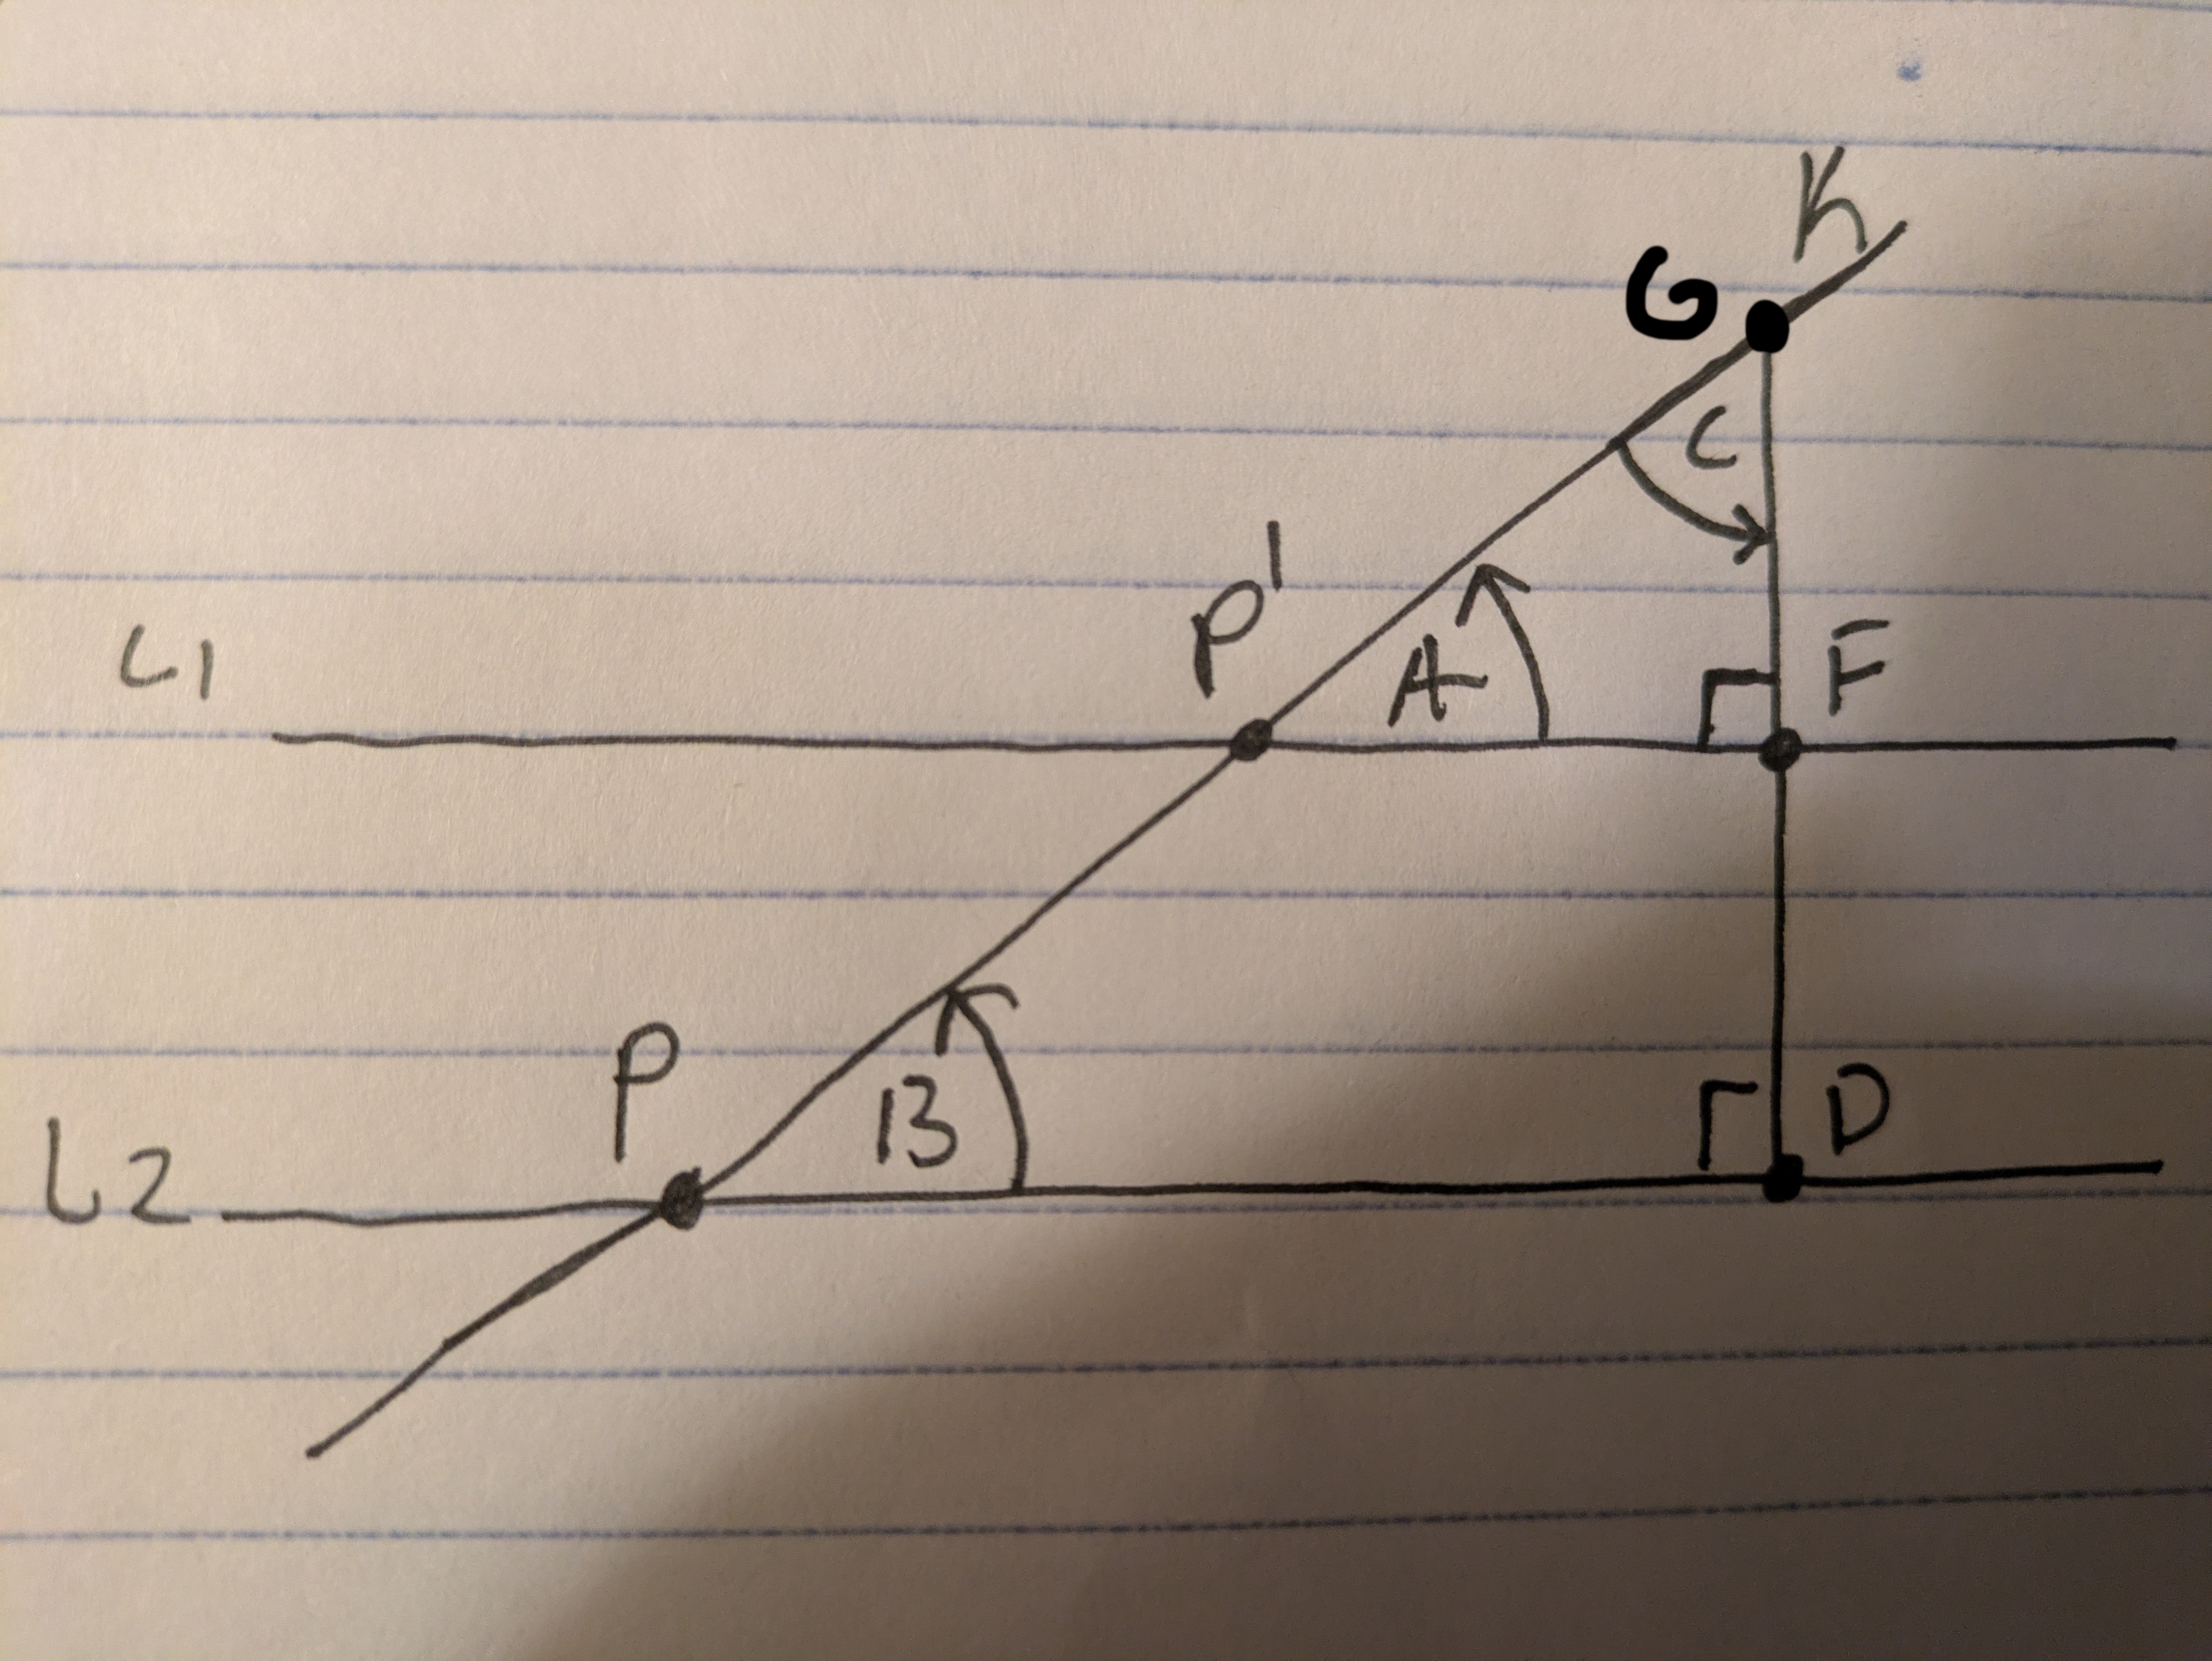
\includegraphics[width=0.6\textwidth]{images/5_5_a.jpg}
\end{figure}

\begin{figure}[h]
    \centering
    \includegraphics[width=0.6\textwidth]{images/5_again.png}
\end{figure}

\begin{figure}[h]
    \centering
    \includegraphics[width=0.6\textwidth]{images/lets_go.png}
\end{figure}

\begin{proof}
    Refer to the figure. Consider the areas enclosed by the right triangles 
        $\triangle P'FG$ and $\triangle PDG$.
    By Problem $10$, the degrees of $\triangle P'FG$ is $90\textdegree + m(A) + m(C) = 180\textdegree$.
    Similarly, the degress of $\triangle PDG$ is $90\textdegree + m(B) + m(C) = 180\textdegree$.
    Then $90\textdegree + m(A) + m(C) = 90\textdegree + m(B) + m(C)$
        and it follows that $m(A) = m(B)$.
\end{proof}

\begin{proof}
    Refer to the text. Then let the parallel segments formed by points $Q, P$ and $N, M$
        be the parallel lines $L_1$, $L_2$. Also let $B$ be the $B$ in our problem.
    Finally, let $\angle NQM$ be $m(B')$.
    It then follows from the text that $m(B) = m(B')$.
\end{proof}

\begin{proof}
    Refer to the figure. Line $D$ is parallel to line $K$.
    The measure of the green angle is equal to $m(A)$ by Problem $13$(b).
    Then $m(A') = m(A)$ by Problem $13$(a).
\end{proof}

\section{Isometries}
\begin{tcolorbox}[title=Problem 1, breakable]
    Show that in a ring, $0a = a0 = 0$.
\end{tcolorbox}

\begin{proof}
    Let $R$ be a ring and $a$ be an arbitrary element in $R$.
    Then
    \begin{align*}
        0a &= 0a + 0 &&\text{Rule 3} \\
            &= 0a + (0a + (-0a)) &&\text{Rule 4} \\
            &= (0a + 0a) + (-0a) &&\text{Rule 2} \\
            &= ((0 + 0)a) + (-0a) &&\text{Rule 6} \\
            &= 0a + (-0a) &&\text{Rule 3} \\
            &= 0 &&\text{Rule 3}
    \end{align*}
    Similarly 
    \begin{align*}
        a0 &= a0 + 0 &&\text{Rule 3} \\
            &= a0 + (a0 + (-a0)) &&\text{Rule 4} \\
            &= (a0 + a0) + (-a0) &&\text{Rule 2} \\
            &= (a(0 + 0)) + (-a0) &&\text{Rule 6} \\
            &= a0 + (-a0) &&\text{Rule 3} \\
            &= 0 &&\text{Rule 3}
    \end{align*}
    Thus $a0 = 0a = 0$.
\end{proof}

\begin{tcolorbox}[title=Problem 2, breakable]
    Prove part d of Theorem 6.1:
    Show that in a ring the additive identity is unique,
        by supposing $0$ and $0'$ satisfy Rule 3
        and proving that $0 = 0'$.
\end{tcolorbox}

\begin{proof}
    Let $R$ be a ring and suppose there exists $0 \in R$
        and $0' \in R$ such that 
        for all $a \in R$, $a + 0 = a$ and $a + 0' = a$.
    Then $a + 0 = a = a + 0'$.
    By Additive Cancellation $0 = 0'$.
\end{proof}

\begin{tcolorbox}[title=Problem 3, breakable]
    Show that in a ring $(-a)b = a(-b) = -(ab)$.
\end{tcolorbox}

\begin{proof}
    Let $R$ be a ring and $a, b \in R$. Then
    \begin{align*}
        0 = (a + (-a))b 
        \iff &0 = ab + (-a)b &&\text{Rule 6} \\
        \iff &-(ab) + 0 = -(ab) + (ab + (-a)b) \\
        \iff &-(ab) = -(ab) + (ab + (-a)b) &&\text{Rule 3} \\
        \iff &-(ab) = (-(ab) + ab) + (-a)b &&\text{Rule 2} \\
        \iff &-(ab) = 0 + (-a)b &&\text{Rule 4} \\
        \iff &-(ab) = (-a)b + 0 &&\text{Rule 1} \\
        \iff &-(ab) = (-a)b &&\text{Rule 3}
    \end{align*}
    Also
    \begin{align*}
        0 = a(b + (-b)) 
        \iff &0 = ab + a(-b) &&\text{Rule 6} \\
        \iff &-(ab) + 0 = -(ab) + ((ab) + a(-b))  \\
        \iff &-(ab) = -(ab) + ((ab) + a(-b)) &&\text{Rule 3} \\
        \iff &-(ab) = (-(ab) + (ab)) + a(-b) &&\text{Rule 2} \\
        \iff &-(ab) = 0 + a(-b) &&\text{Rule 4} \\
        \iff &-(ab) = a(-b) + 0 &&\text{Rule 1} \\
        \iff &-(ab) = a(-b) &&\text{Rule 3}
    \end{align*}
    Thus $(-a)b = a(-b) = -(ab)$.
\end{proof}

\begin{tcolorbox}[title=Problem 4, breakable]
    Show that in a ring $(-a)(-b) = ab$.
\end{tcolorbox}

\begin{proof}
    \begin{align*}
        (-a)(-b) + -(ab) &= a(-(-b)) + a(-b) && \text{Rule 6} \\
                        &= a((-(-b)) + (-b)) && \text{Rule 2} \\
                        &= a \cdot 0 && \text{Rule 4} \\
                        &= 0 && \text{Rule 3}
    \end{align*}
    Thus $(-a)(-b) = ab$.
\end{proof}

\begin{tcolorbox}[title=Problem 5, breakable]
    Prove the following facts about subtraction in a ring $R$,
    where $a, b, c \in R$.

    (a) $a - a = 0$.

    (b) $a(b - c) = ab - ac$.

    (c) $(b - c)a = ba - ca$.
\end{tcolorbox}

\begin{proof}
    Let $R$ be a ring and $a, b, c \in R$.
    Then $a - a = a + (-a) = 0$ Rule 4.
    Also, $a(b - c) = a(b + (-c)) = ab + a(-c)$ Rule 6.
    Then, $ab + a(-c) = ab + -(ac) \text{ Problem 3 } = ab - ac$.
    Similarly, $(b - c)a = (b + (-c))a = ba + (-c)a$ Rule 6.
    Then, $ba + (-c)a = ba + -(ca) \text{ Problem 3 } = ba - ca$.
\end{proof}

\begin{tcolorbox}[title=Problem 8, breakable]
    We generalize Exercises 6 and 7: Let $R$
    be any commutative ring (other than the zero ring).
    Define $M_2(R)$ as the set of $2 \times 2$
    matrices with entries from $R$. Show that $M_2(R)$
    is a ring which is not commutative. (Note that 
    for the most part the proofs in Exercises 6 and 
    7 life over without change.)
\end{tcolorbox}

\begin{proof}
    Let $R$ be a ring and 
    \[a, b, c, e, f, g, h, i, j, k, l \in R\]
    We first show associativity with respect to $+$.
    \[\begin{bmatrix}
        a & b \\
        c & d
    \end{bmatrix} \in M_2(R) \text{, }
    \begin{bmatrix}
        c & f \\
        g & h
    \end{bmatrix} \in M_2(R) \text{ and }
    \begin{bmatrix}
        i & j \\
        k & l
    \end{bmatrix} \in M_2(R)\]
    Then 
    \[\begin{bmatrix}
        a & b \\
        c & d
    \end{bmatrix} + \begin{bmatrix}
        c & f \\
        g & h
    \end{bmatrix} = \begin{bmatrix}
        a+c & b+f \\
        c+g & d+h
    \end{bmatrix} = \begin{bmatrix}
        c+a & f+b \\
        g+c & h+d
    \end{bmatrix} = \begin{bmatrix}
        c & f \\
        g & h
    \end{bmatrix} + \begin{bmatrix}
        a & b \\
        c & d
    \end{bmatrix}\]
    We now show associativity with respect to $+$.
\[\left(\begin{bmatrix}
        a & b \\
        c & d
    \end{bmatrix} + \begin{bmatrix}
        c & f \\
        g & h
    \end{bmatrix}\right) + \begin{bmatrix}
        i & j \\
        k & l
    \end{bmatrix} = \begin{bmatrix}
        a+c & b+f \\
        c+g & d+h
    \end{bmatrix} +\begin{bmatrix}
        i & j \\
        k & l
    \end{bmatrix} = \begin{bmatrix}
        (a+c)+i & (b+f)+j \\
        (c+g)+k & (d+h)+l
    \end{bmatrix}\] \[= \begin{bmatrix}
        a+(c+i) & b+(f+j) \\
        c+(g+k) & d+(h+l)
    \end{bmatrix} = \begin{bmatrix}
        a & b \\
        c & d
    \end{bmatrix} + \begin{bmatrix}
        c+i & f+j \\
        g+k & h+l
    \end{bmatrix} = \begin{bmatrix}
        a & b \\
        c & d
    \end{bmatrix} + \left(\begin{bmatrix}
        c & f \\
        g & h
    \end{bmatrix} + \begin{bmatrix}
        i & j \\
        k & l
    \end{bmatrix}\right)\]
    We now show the existence of an additive inverse.
    \[\begin{bmatrix}
        a & b \\
        c & d
    \end{bmatrix} -\begin{bmatrix}
        a & b \\
        c & d
    \end{bmatrix} = \begin{bmatrix}
        a-a & b-b \\
        c-c & d-d
    \end{bmatrix} = \begin{bmatrix}
        0 & 0 \\
        0 & 0
    \end{bmatrix}\]
    We now show the existence of the additive identity.
    \[\begin{bmatrix}
        a & b \\
        c & d
    \end{bmatrix} + \begin{bmatrix}
        0 & 0 \\
        0 & 0
    \end{bmatrix} = \begin{bmatrix}
        a+0 & b+0 \\
        c+0 & d+0
    \end{bmatrix} = \begin{bmatrix}
        a & b \\
        c & d
    \end{bmatrix}\]
    We now show left distributivity.
    \[
    \begin{bmatrix}
        a & b \\
        c & d
    \end{bmatrix}
    \left(
    \begin{bmatrix}
        e & f \\
        g & h
    \end{bmatrix}
    +
    \begin{bmatrix}
        i & j \\
        k & l
    \end{bmatrix}
    \right)
    =
    \begin{bmatrix}
        a & b \\
        c & d
    \end{bmatrix}
    \begin{bmatrix}
        e+i & f+j \\
        g+k & h+l
    \end{bmatrix}
    =
    \begin{bmatrix}
        a(e+i) + b(g+k) & a(f+j) + b(h+l) \\
        c(e+i) + d(g+k) & c(f+j) + d(h+l)
    \end{bmatrix}
    \]
    \[
    =
    \begin{bmatrix}
        ae + bg & af + bh \\
        ce + dg & cf + dh
    \end{bmatrix}
    +
    \begin{bmatrix}
        ai + bk & aj + bl \\
        ci + dk & cj + dl
    \end{bmatrix}
    =
    \begin{bmatrix}
        a & b \\
        c & d
    \end{bmatrix}
    \begin{bmatrix}
        e & f \\
        g & h
    \end{bmatrix}
    +
    \begin{bmatrix}
        a & b \\
        c & d
    \end{bmatrix}
    \begin{bmatrix}
        i & j \\
        k & l
    \end{bmatrix}.
    \]
    We now show right distributivity.
    \[
    \left(
    \begin{bmatrix}
        e & f \\
        g & h
    \end{bmatrix}
    +
    \begin{bmatrix}
        i & j \\
        k & l
    \end{bmatrix}
    \right)
    \begin{bmatrix}
        a & b \\
        c & d
    \end{bmatrix}
    =
    \begin{bmatrix}
        e+i & f+j \\
        g+k & h+l
    \end{bmatrix}
    \begin{bmatrix}
        a & b \\
        c & d
    \end{bmatrix}
    =
    \begin{bmatrix}
        (e+i)a + (f+j)c & (e+i)b + (f+j)d \\
        (g+k)a + (h+l)c & (g+k)b + (h+l)d
    \end{bmatrix}
    \]
    \[
    =
    \begin{bmatrix}
        ea + fc & eb + fd \\
        ga + hc & gb + hd
    \end{bmatrix}
    +
    \begin{bmatrix}
        ia + jc & ib + jd \\
        ka + lc & kb + ld
    \end{bmatrix}
    =
    \begin{bmatrix}
        e & f \\
        g & h
    \end{bmatrix}
    \begin{bmatrix}
        a & b \\
        c & d
    \end{bmatrix}
    +
    \begin{bmatrix}
        i & j \\
        k & l
    \end{bmatrix}
    \begin{bmatrix}
        a & b \\
        c & d
    \end{bmatrix}
    \]
    We now show matrix multiplication is not commutative 
        by giving a counterexample.
    Consider
    \[
    \begin{bmatrix}
    1 & 2 \\
    0 & 1
    \end{bmatrix}
    \begin{bmatrix}
    1 & 0 \\
    3 & 1
    \end{bmatrix}
    =
    \begin{bmatrix}
    1+6 & 2 \\
    3 & 1
    \end{bmatrix}
    =
    \begin{bmatrix}
    7 & 2 \\
    3 & 1
    \end{bmatrix}
    \]
    But multiplying the same matrices in the opposite order gives
    \[
    \begin{bmatrix}
    1 & 0 \\
    3 & 1
    \end{bmatrix}
    \begin{bmatrix}
    1 & 2 \\
    0 & 1
    \end{bmatrix}
    =
    \begin{bmatrix}
    1 & 2 \\
    3 & 7
    \end{bmatrix}.
    \]
    Since
    \[
    \begin{bmatrix}
    7 & 2 \\
    3 & 1
    \end{bmatrix}
    \neq
    \begin{bmatrix}
    1 & 2 \\
    3 & 7
    \end{bmatrix}
    \]
    matrix multiplication is not commutative.
\end{proof}

Let $R = \{0, a, \ldots\}$ such that $0 \ne a$.
\[
A = \begin{bmatrix} 0 & a \\ 0 & 0 \end{bmatrix}, \quad
B = \begin{bmatrix} 0 & 0 \\ a & 0 \end{bmatrix}
\]
\[
AB = \begin{bmatrix} a^2 & 0 \\ 0 & 0 \end{bmatrix} \neq 
BA = \begin{bmatrix} 0 & 0 \\ 0 & a^2 \end{bmatrix}
\]

\begin{tcolorbox}[title=Problem 9, breakable]
    Check that Example 6.14 is indeed a ring; that is,
    let $C[0, 1]$ be a set of functions defined from the closed 
    unit interval $[0, 1]$ to the real numbers that 
    are continuous. Define the sum and product of two 
    functions point-wise: $(f + g)(x) = f(x) + g(x)$
    and $(fg)(x) = f(x)g(x)$. Show that $C[0, 1]$ is a 
    commutative ring. (You may use theorems from calculus).
\end{tcolorbox}

\begin{proof}
    Let $x \in [0, 1]$ and $f, g, l : [0, 1] \longrightarrow \mathbb{R}$.
    Since $f(x), g(x), l(x) \in \mathbb{R}$ and $\mathbb{R}$ is a ring, standard ring operations (associativity, distributivity, etc.) hold.
    We first show commutativity over addition
    \[
    (f + g)(x) = f(x) + g(x) = g(x) + f(x) = (g + f)(x)
    \]
    Next, associativity over addition
    \[
    ((f + g) + l)(x) = (f + g)(x) + l(x) = f(x) + g(x) + l(x) = f(x) + (g + l)(x) = (f + (g + l))(x).
    \]
    Existence of additive inverses
    \[
    (f + (-f))(x) = f(x) + (-f(x)) = 0
    \]
    Additive identity
    \[
    (f + 0)(x) = f(x) + 0(x) = f(x)
    \]
    Commutativity of multiplication
    \[
    (fg)(x) = f(x) g(x) = g(x) f(x) = (gf)(x)
    \]
    Associativity of multiplication
    \[
    ((fg)l)(x) = (fg)(x) l(x) = f(x) g(x) l(x) = f(x) (gl)(x) = (f(gl))(x)
    \]
    Distributivity from the left
    \[
    f(g + l)(x) = f(x)(g + l)(x) = f(x)(g(x) + l(x)) = f(x)g(x) + f(x)l(x) = (fg + fl)(x)
    \]
    Distributivity from the right
    \[
    (f + g)l(x) = (f + g)(x) \, l(x) = (f(x) + g(x))l(x) = f(x)l(x) + g(x)l(x) = (fl + gl)(x)
    \]
\end{proof}

\begin{tcolorbox}[title=Problem 11, breakable]
    Let $\mathbb{C}$ be the complex numbers. That inverse
    \[\mathbb{C} = \{a + bi \mid a, b, \in \mathbb{R}\}\]
    where $i$ is the square root of $-1$ (that is, $i \cdot i = 1$).
    Here 
    \[(a + bi) + (c + di) = (a + c) + (bi + di)\]
    and 
    \[(a + bi)(c + di) = (ac - bd) + (ad + bc)i\]
    Show that $\mathbb{C}$ is a commutative ring.
\end{tcolorbox}

\begin{proof}
    Let $a + bi, c + di, e + fi \in \mathbb{C}$.
    We first show commutativity over addition
    \[
    (a + bi) + (c + di) = (a + c) + (bi + di) = (c + a) + (di + bi) = (c + di) + (a + bi)
    \]
    Next, associativity over addition
    \[
    ((f + g) + l)(x) = (f + g)(x) + l(x) = f(x) + g(x) + l(x) = f(x) + (g + l)(x) = (f + (g + l))(x).
    \]
    Existence of additive inverses
    \[
    (f + (-f))(x) = f(x) + (-f(x)) = 0
    \]
    Additive identity
    \[
    (f + 0)(x) = f(x) + 0(x) = f(x)
    \]
    Commutativity of multiplication
    \[
    (fg)(x) = f(x) g(x) = g(x) f(x) = (gf)(x)
    \]
    Associativity of multiplication
    \[
    ((fg)l)(x) = (fg)(x) l(x) = f(x) g(x) l(x) = f(x) (gl)(x) = (f(gl))(x)
    \]
    Distributivity from the left
    \[
    f(g + l)(x) = f(x)(g + l)(x) = f(x)(g(x) + l(x)) = f(x)g(x) + f(x)l(x) = (fg + fl)(x)
    \]
    Distributivity from the right
    \[
    (f + g)l(x) = (f + g)(x) \, l(x) = (f(x) + g(x))l(x) = f(x)l(x) + g(x)l(x) = (fl + gl)(x)
    \]
\end{proof}

\begin{tcolorbox}[title=Problem 15, breakable]
    Verify that 6.10 is a ring.
    Namely, let $R$ and $S$ be arbitrary rings.
    Define addition and subtraction appropriately
        to make $R \times S$ a ring,
        where $R \times S$ is the set of ordered pairs
        with the first entry from $R$ and second entry 
        from $S$. 
    Now generalize this to the set $R_1 \times R_2 \times \cdots R_n$
    of $n$-tuples with entries from the rings $R_i$.
    This new ring is called the \textbf{direct product}
    of the rings $R_i$.
\end{tcolorbox}
\section{Area and Applications}
\subsection{Area of a Disc of Radius $r$}

\begin{tcolorbox}[title=Problem 3, breakable]
    (a) Suppose that the sides of a rectangles $S$ have lengths 
        $r$ and $s$. What are the lengths of the sides  of the 
        rectangle $F_{a, b}(S)$, i.e. of the rectangle obtained 
        by the mixed dilation $F_{a, b}$?

    (b) What is the area of $F_{a, b}$?

    (c) If $S$ is a bounded region in the plane with area $A$,
        what is the area of $F_{a, b}(S)$?
\end{tcolorbox}

\textbf{Solution (a):}
\[F_{a, b}(S) \text{ has } ar \text{ width and } bs \text{ height.}\]
\textbf{Solution (b):}
\[\text{area}= ar \cdot bs = ab(rs)\]
\textbf{Solution (c):}
\[F_{a, b}(S) = ab(A)\]

\begin{tcolorbox}[title=Problem 4, breakable]
    (a) Show that the set of points $(u, v)$ satisfying the equation
        \[\left(\frac{u}{a}\right)^2 + \left(\frac{v}{b}\right)^2 = 1\]
        is the image of the circle of radius $1$ centered at $O$ under 
        the map $F_{a, b}$.

    (b) Let $a = 3$ and $b = 2$. Sketch this set, which is called an 
        \textbf{ellipse}.

    (c) Can you guess and motivate your guess as to what the area of the 
        region bounded by the ellipse in $(a)$ should be.
\end{tcolorbox}

\begin{proof}
    Let $C$ be the set of points making up the circle with radius $r = 1$ and center $O$.
    Let $P$ be an arbitrary point in $C$. Since $r = 1$, $d(O, P) = 1$.
    Let $L_1$ and $L_2$ be the vertical and horizontal lines through $O$, respectively.
    Drop perpendiculars from $P$ to $L_1$ and $L_2$, 
        and let $Q$ and $R$ be the feet of these perpendiculars on $L_1$ and $L_2$, respectively.
    Then $\triangle OQR$ is a right triangle with hypotenuse $\overline{OP}$, 
        and legs $\overline{OQ}$ and $\overline{OR}$ lying along $L_1$ and $L_2$.
    Let $u = d(OQ), v = d(OR)$ and by Pythagoras' Theorem $u^2 + v^2 = 1$.
    By applying the mapping $F_{a, b}$ to $\overline{OQ}, \overline{OR}$ 
        lengths $u, v$ are scaled by $\frac{1}{a}, \frac{1}{b}$ respectively
        we get $\left(\frac{u}{a}\right)^2 + \left(\frac{v}{b}\right)^2 = 1$.
\end{proof}

\textbf{Solution (b):}

\begin{figure}[h]
    \centering
    \includegraphics[width=0.6\textwidth]{images/ellipse.png}
\end{figure}

\textbf{Solution (c):}

Start with a circle of radius $r = 1$
    and suppose its area $A = \pi$.
We can subdivide this region into small squares with width $x$ and height $y$.
By Problem $3$ applying a $F_{a, b}$ to $x, y$ gives $ax, by$
    resulting in an area of $ab(xy)$.
Applying these dilations to the entire unit circle gives $ab\pi$.

\begin{tcolorbox}[title=Problem 7, breakable]
    Write up a discussion of how to give coordinates $(x, y, z)$ to 
    a point in $3-$space. In terms of these coordinates, what would the 
    effect of dilation by $r$?
\end{tcolorbox}

\textbf{Solution:}

Let $L_1, L_2, L_3$ be perpendicular lines intersecting at a point $O$.
Let $P$ be an arbitrary point in space.
Let the distances of the segments formed by dropping perpendiculars
    from $P$ to $L_1, L_2, L_3$ on one side be $(x, y, z)$.
On the opposite side, they are $(-x, -y, -z)$.

Let $V$ be the volume of a region in $3$-space. The effect of 
a dilation by $r$ would be to multiply the volume by $r^3$, giving $r^3 V$.

\begin{tcolorbox}[title=Problem 8, breakable]
    Generalize the discussion of this section to the $3$-dimensional
    case. Specifically:

    (a) Under dilation by $r$, how does the volume of a cube change?

    (b) How does the volume of a rectangle box with sides $a, b, c$ change?
        Draw a picture, say $r = \frac{1}{2}, r = 2, r = 3$, arbitrary $r$.

    (c) How would the volume of a $3-$dimensional solid change under 
        dilation by $r$?

    (d) The volume of the solid ball of radius $1$ in $3-$space is equal 
        to $\frac{4}{3} \pi$. What is the volume of the ball of radius 
        $r$ in $3-$space?
\end{tcolorbox}

\textbf{Solution (a):}

Under dilation $r$ the new volume $V' = r^3 V$ where $V$ is the volume 
    of the original cube.

\textbf{Solution (b):}

\begin{figure}[h]
    \centering
    \includegraphics[width=0.6\textwidth]{images/half_rect.png}
\end{figure}

\begin{figure}[h]
    \centering
    \includegraphics[width=0.6\textwidth]{images/2_rect.png}
\end{figure}

\begin{figure}[h]
    \centering
    \includegraphics[width=0.6\textwidth]{images/3_rect.png}
\end{figure}

There are three cases for an arbitrary $r$ shown below
    depending on if $r < 1, r = 1, r > 1$.
If $r = 1$ the rectangle doesn't change that image isn't shown.
The first image shows if $r < 1$ and the second shows if $r > 1$.

\begin{figure}[h]
    \centering
    \includegraphics[width=0.6\textwidth]{images/arb1_rect.png}
\end{figure}

\begin{figure}[h]
    \centering
    \includegraphics[width=0.6\textwidth]{images/arb2_rect.png}
\end{figure}

\textbf{Solution (c):}

Let $V$ be the volume of a solid. Under dilation $r$ the volume of the 
new solid is 
\[r^3 \cdot V\]

\textbf{Solution (d):}

\[V = r^3 \cdot \frac{4}{3}\pi\]

\begin{tcolorbox}[title=Problem 9, breakable]
    Write down the equation of a sphere of radius $r$ centered at the 
    origin in $3-$space.
\end{tcolorbox}

\textbf{Solution:}
\[a^2 + b^2 + c^2 = r^2\]

\begin{tcolorbox}[title=Problem 10, breakable]
    How would you define the volume of a rectangle solid whose sides 
    have lengths $a, b, c$.
\end{tcolorbox}

\begin{definition}
    Let the volume $V$ of a rectangle $R$ be defined as
    \[V = a \cdot b \cdot c\]
\end{definition}

\begin{tcolorbox}[title=Problem 11, breakable]
    Let $a, b, c$ be positive numbers. Let $\mathbb{R}^3$ be $3-$space,
    that is, the set of all triples of numbers $(x, y, z)$. Let 
    \[F_{a, b, c}: \mathbb{R^3} \rightarrow \mathbb{R}^3\]
    be the mapping
    \[(x, y, z) \rightarrow (ax, by, cz)\]
    Thus $F_{a, b, c}$ is a generalization to a $3-$space of our mixed 
    dilation $F_{a, b}$.

    (a) What is the image of a cube whose sides have length $1$ under $F_{a, b, c}$?
    
    (b) A rectangular box $S$ has sides of length $r, s, t$ respectively.
        What are the lengths of the sides of the image $F_{a, b}(S)$?
        What is the volume of $F_{a, b, c}(S)$?

    (c) Let $S$ be a solid in $3-$space, and let $V$ be its volume. 
        In terms of $V$, $a, b, c$ what is the volume of the image $S$
        under $F_{a, b, c}$?
\end{tcolorbox}

\textbf{Solution (a):}

The image of a cube whose sides have length $1$ under $F_{a, b, c}$
is a rectangular prism of side lengths $a, b, c$.

\textbf{Solution (b):}

The lengths of the sides of the image $F_{a, b}(S)$ is $ar, bs, t$.
The volume of $F_{a, b, c}(S)$ is $V = abc(rst)$.

\textbf{Solution (c):}

Let $V'$ be the volume of the image.
\[V' = abc V\]

\begin{tcolorbox}[title=Problem 12, breakable]
    What is the volume of the solid in $3-$space consisting of all points
    $(x, y, z)$ satisfying the inequality
    \[\left(\frac{x}{3}\right)^2 + \left(\frac{y}{2}\right)^2 + \left(\frac{z}{7}\right)^2 \le 1\]
\end{tcolorbox}

\textbf{Solution:}
\[V = 3 \cdot 2 \cdot 7 \cdot \frac{4}{3} \pi\]

\begin{tcolorbox}[title=Problem 14, breakable]
    Let $a, b, c$ be numbers $>0$. What is the volume of the solid 
    in $3-$space consisting of all points $(x, y, z)$ satisfying
    the inequality
    \[\left(\frac{x}{a}\right)^2 + \left(\frac{y}{b}\right)^2 + \left(\frac{z}{c}\right)^2 \le 1\]
\end{tcolorbox}

\textbf{Solution:}
\[V = a \cdot b \cdot c \cdot \frac{4}{3} \pi\]

\begin{tcolorbox}[title=Problem 15, breakable]
    What about $4-$space? $n-$space for arbitrary $n$?
\end{tcolorbox}

Let $V'$ be volume of $4-$D sphere.
The volume of the solid 
    in $4-$space consisting of all points $(x, y, z, d)$ satisfying
    the inequality
\[\left(\frac{x}{a}\right)^2 + \left(\frac{y}{b}\right)^2 
+ \left(\frac{z}{c}\right)^2 + \left(\frac{p}{d}\right)^2 \le 1\]
has volume
\[V = a \cdot b \cdot c \cdot d \cdot V'\]

Let $V'$ be volume of $n-$D sphere.
The volume of the solid 
    in $n-$space consisting of all points $(x_1, x_2, x_3, \ldots, x_n)$ satisfying
    the inequality
\[\left(\frac{y_1}{x_1}\right)^2 + \left(\frac{y_2}{x_2}\right)^2 
+ \left(\frac{y_3}{x_3}\right)^2 + \ldots +  \left(\frac{y_n}{x_n}\right)^2 \le 1\]
has volume
\[V = x_1 \cdot x_2 \cdot x_3 \cdot \ldots \cdot x_n \cdot V'\]
\section{Coordinates and Geometry}
\begin{tcolorbox}[title=Problem 1, breakable]
    Prove that if $R$ is a commutative ring 
    and $a \in R$ is a zero divisor, then $ax$
    is also a zero divisor or $0$, for all $x \in R$.
\end{tcolorbox} 

\begin{proof}
    Suppose $R$ is a commutative ring and $a \in R$ is a zero divisor.
    Then there exists $b \in R$ with $b \ne 0$ such that $ab = 0$.
    Now, let $x$ be an arbitrary element of $R$.
    If $ax = 0$, then we are done.
    Suppose $ax \ne 0$.
    Then $(ax)b = a(xb) = (ab)x = 0$.   
    Since $b \ne 0$, it follows that $ax$ is a zero divisor.
\end{proof}

\begin{tcolorbox}[title=Problem 6, breakable]
    Use Fermat's Little Theorem 8.7 to find 
    $[6]^{-1}$ in $\mathbb{Z}_{19}$.
\end{tcolorbox} 

\begin{proof}
    In $\mathbb{Z}_{19}$ the theorem asserts that 
        $[6]^{18} = [1]$.
    But then $[6][6]^{17} = [1]$ so $[6]^{-1} = [6]^{17} = [16]$.
\end{proof}

\begin{tcolorbox}[title=Problem 7, breakable]
    Use Euclid's Algorithm to find $[36]^{-1}$ in $\mathbb{Z}_{101}$.
\end{tcolorbox} 

\begin{proof}
    First notice $1 = 5 \cdot 101 - 14 \cdot 36$.
    Thus $-14 \cdot 36 = 1 \pmod 101$.
    Therefor $[36]^{-1} = [-14] = [87]$.
\end{proof}

\begin{tcolorbox}[title=Problem 9, breakable]
    Suppose that $b \in R$, a non-commutative ring 
    with unity. Suppose that $ab = bc = 1$;
    that is, $b$ has a \textbf{right inverse} $c$
    and a \textbf{left inverse} $a$. Prove that 
    $a = c$ and that $b$ is a unit.
\end{tcolorbox} 

\begin{proof}
    Now $a = a \cdot 1 = a(bc) = (ab)c = 1 \cdot c = c$ as required.
    It directly follows that $b$ is a unit.
\end{proof}

\begin{tcolorbox}[title=Problem 11, breakable]
    Let $R$ be a commutative ring with unity.
    Suppose that $n$ is the least postivive integer 
    for which we get $0$ when we add $1$ to itself $n$
    times; we then say $R$ has a \textbf{characteristic n}.
    If there exists no such $n$, we say that $R$ has 
    \textbf{characteristic 0}. For example, the 
    characteristic of $\mathbb{Z}_5$ is $5$ because 
    $1 + 1 + 1 + 1 + 1 = 0$, whereas 
    $1 + 1 + 1 + 1 \ne 0$. (Note that here we 
    have suppressed `[' and `]'.)

    (a) Show that, if the characteristic of a commutative ring with unity $R$ 
        is $n$ and $a$ is \emph{any} of $R$, then $na = 0$. (Recall that 
        $na = \underbrace{a + a + \cdots + a}_{n \text{ times}}$.)

    (b) What are the characteristics of $\mathbb{Q}, \mathbb{R}, \mathbb{Z}_{17}$?

    (c) Prove that if a field $F$ has characteristic $n$, where $n > 0$, 
        then $n$ is a prime integer.
\end{tcolorbox} 

\begin{proof}
    Notice
    \[
    na = \underbrace{a + a + \cdots + a}_{n \text{ times}}
       = a(\underbrace{1 + 1 + \cdots + 1}_{n \text{ times}})
       = a \cdot 0
       = 0.
    \]
\end{proof}

\textbf{Solution:} $\mathbb{Q}$ and $\mathbb{R}$ have characteristic $0$.
Finally, $\mathbb{Z}_{17}$ has characteristic $17$.

\begin{proof}
    Suppose $F$ is a field with characteristic $n$ where $n > 0$.
    For contradiction, suppose $n$ is not prime, so $n = ab$ for some
    $a,b$ with $1 < a,b < n$.
    Since $F$ is a field, it has no zero divisors, so
    $
    0 = n \cdot 1 = (a \cdot 1)(b \cdot 1)
    $.
    Now either $a \cdot 1 = 0$ or $b \cdot 1 = 0$ either of which is a contradiction.
\end{proof}

\begin{tcolorbox}[title=Problem 12, breakable]
    Consider the commutative ring $F = \{0, 1, \alpha, 1 + \alpha\}$,
    where $0$ is the additive identity, $1$ is the mutliplicative identity,
    $x + x = 0$, for all $x \in F$, and $\alpha^2 = 1 + \alpha$.

    (a) Write out explicitly the addition and mutliplication tables for $F$.

    (b) Prove that $F$ is a field.

    (c) Because $F$ has four elements, you might expect $F$ would be the ``same''
        as the ring $\mathbb{Z}_4$. Show this is false, by computing the characteristics 
        of $F$ and $\mathbb{Z}_4$ (see the previous exercise).
\end{tcolorbox} 

\textbf{Solution (a):}
\[
\begin{array}{c|cccc}
+ & 0 & 1 & \alpha & 1+\alpha \\
\hline
0 & 0 & 1 & \alpha & 1+\alpha \\
1 & 1 & 0 & 1+\alpha & \alpha \\
\alpha & \alpha & 1+\alpha & 0 & 1 \\
1+\alpha & 1+\alpha & \alpha & 1 & 0
\end{array}
\]
\[
\begin{array}{c|cccc}
\cdot & 0 & 1 & \alpha & 1+\alpha \\
\hline
0 & 0 & 0 & 0 & 0 \\
1 & 0 & 1 & \alpha & 1+\alpha \\
\alpha & 0 & \alpha & 1+\alpha & 1 \\
1+\alpha & 0 & 1+\alpha & 1 & \alpha
\end{array}
\]

\begin{proof}
    Notice $1 \cdot 1 = 1$ and
    \[
    \alpha \cdot (1+\alpha) = \alpha + \alpha^2 = \alpha + (\alpha+1) = 1.
    \]
    Since every nonzero element has a multiplicative inverse, $F$ is a field.
\end{proof}

\textbf{Solution (c):}
In $F$, $1 + 1 = 0$ but in $\mathbb{Z}_4$, $1 + 1 + 1 + 1 = 0$ and $1 + 1 \ne 0$. So they are not the same ring.

\begin{tcolorbox}[title=Problem 14, breakable]
    Prove that $\mathbb{Z}_m$ is the union of three mutually disjoint subsets: its 
    zero divisors, its units, and $\{0\}$. Show by example that this is false 
    for an arbitrary commutative ring.
\end{tcolorbox} 

\begin{proof}
    $\{0\}$ is clearly not a zero divisor or a unit in $\mathbb{Z}_m$.
    Now, suppose $a \in \mathbb{Z}_m$ is a zero divisor and a unit.
    Then there exists $b \ne 0$ such that $ab = 0$.
    But then $a^{-1} ab = a^{-1} 0 \implies 1 \cdot b = 0 \implies b = 0$,
        a contradiction.

    Now suppose $a \in \mathbb{Z}_m$ and $a \ne 0$.
    If $\gcd(a, m) = 1$ then $a$ is a unit.
    Suppose $\gcd(a, m) = d > 1$.
    Then, there exists $k_1, k_2 \in \mathbb{Z}$ such that $a = d k_1$ and $m = d k_2$.
    Then $a = d k_1 \iff a k_2 = d k_2 k_1 = m k_1 \equiv 0 \pmod m$.
    Thus $a$ is either a unit or a zero divisor.

    A counterexample is the trivial ring.
\end{proof}
\section{Operations on Points}
\begin{tcolorbox}[title=Problem 2, breakable]
    (a) Why does every non-zero complex number have exactly 
        two square roots?

    (b) Given part a, check that the proof of the quadratic formula 
        obtained in Exercise 9.1 still holds in $\mathbb{C}[x]$.

    (c) Use the quadratic formula to compute the roots of the polynomials 
        $x^2 - (3 + 2i)x + (1 + 3i)$ and $x^2 - (1 + 3i)x + (-2 + 2i)$.
\end{tcolorbox} 

\textbf{Solution (a):}
The book states a non-zero complex number $\alpha = |\alpha|(\cos \theta + i \sin \theta) = |\alpha|e^{i \theta}$
has a square root $\beta = |\alpha|^{1/2}(\cos(\theta/2) + i \sin(\theta/2))$.
Any square root of $\alpha$ must have argument $\theta/2 \pmod{\pi}$, so the only square roots are $\beta$ and $-\beta$.

\textbf{Solution (b):} Checked, and it still holds.

\textbf{Solution (c):}
The roots of $x^2 - (3 + 2i)x + (1 + 3i)$ are
$\frac{-(-(3 + 2i)) \pm \sqrt{(-(3 + 2i))^2 - 4(1 + 3i)}}{2}$.
The roots of $x^2 - (1 + 3i)x + (-2 + 2i)$ are
$\frac{-(-(1 + 3i)) \pm \sqrt{(-(1 + 3i))^2 - 4(-2 + 2i)}}{2}$.

\begin{tcolorbox}[title=Problem 3, breakable]
    Give examples of two different polynomials in $\mathbb{Z}_5[x]$
    that are identical as functions over $\mathbb{Z}_5$.
    This shows that equality of polynomials in $F[x]$ cannot be 
    thought of as equality of the corresponding polynomial \emph{functions}.
    (See the Quick Exercise in Section 4.1 for $F = \mathbb{Z}_2$ case, and 
    Exercise 4.12 for the $F = \mathbb{Z}_3$.)
\end{tcolorbox} 

\textbf{Solution:} By Fermat's little Theorem in $\mathbb{Z}_5$
the polynomials $x^5$ and $x$ are equivalent for all $x$.

\begin{tcolorbox}[title=Problem 4, breakable]
    Consider the polynomial $f = x^3 + 3x^2 + 2x \in \mathbb{Z}_6[x]$.
    Show that this polynomial has more than three roots in $\mathbb{Z}_6$.
    Why doesn't this contradict the Root Theorem?
\end{tcolorbox} 

\textbf{Solution:} We can manually check that $x = 0, 1, 2, 3$ are roots.
The Root Theorem is about fields and $\mathbb{Z}_6$ is not a field.

\begin{tcolorbox}[title=Problem 8, breakable]
    Show that if $f$ is a polynomial with real coefficients and $\alpha = s + ti$
    is a root of $f$ in $\mathbb{C}$, then so is $\overline{\alpha} = s - ti$.
\end{tcolorbox} 

\begin{proof}
    Let $\alpha, \beta$ be complex numbers.
    We have the following two properties of the algebra of complex numbers 
    \begin{enumerate}
        \item $\overline{\alpha} + \overline{\beta} = \overline{\alpha + \beta}$.
        \item $\overline{\alpha\beta} = \overline{\alpha}\,\overline{\beta}$.
    \end{enumerate}
    Suppose $f$ has real coefficients. 
    Note that for a coefficient $x \in R$, $x = \overline{x}$.
    From this it clearly follows that
    $f(\overline{\alpha}) = \overline{f(\alpha)}$.
    But then suppose $f(\alpha) = 0$ and it follows that
    $f(\overline{\alpha}) = \overline{f(\alpha)} = \overline{0} = 0$.
\end{proof}

\begin{tcolorbox}[title=Problem 12, breakable]
    In this exercise, we describe the cubic formula for factoring an arbitrary polynomial
    of degree $3$ in $\mathbb{R}[x]$. This version of the formula is called the 
    \emph{Cardano-Tartaglia} formula, after two 16th-century Italian mathematicians 
    involved in its discovery. Consider the polynomial $f = x^3 + ax^2 + bx + c \in \mathbb{R}[x]$
    (by dividing by the leading coefficient if necessary, we have assumed without loss 
    of generality that it is $1$).

    (a) Show that the change in variables $x = y - \frac{1}{3}a$ changes $f$ into 
        a cubic polynomial that lacks a square term; that is, a 
        polynomial of the form $g = f(y - \frac{1}{3}a) = y^3 + py + q = 0$.
        \emph{Note: } This process is called \emph{depressing the conic}. Clearly 
        we can solve $f = 0$ for $x$ if and only if we can solve $g = 0$ for $y$.

    (b) Find explicit solutions $u, v$ to the pair of simultaneous equations 
        \textcircled{1} $v^3 - u^3 = q$ and \textcircled{2} $uv = \frac{1}{3}p$.

    (c) Prove the identity $(u - v)^3 + 3uv(u - v) + (v^3 - u^3) = 0$ and 
        use it to show that $y = u - v$ is a solution to the cubic equation 
        $y^3 + py + q = 0$.

    (d) Let $D = q^2 + \frac{3p^3}{27}$. (This is called the \emph{discriminant} of the conic.)
        Conclude that $y = \sqrt[3]{\frac{-q + \sqrt{D}}{2}} - \sqrt[3]{\frac{q + \sqrt{D}}{2}}$
        is a root for $g = 0$. (This is just $u - v$.)
\end{tcolorbox} 


\begin{proof}
\begin{align*}
    f\Bigl(y - \frac{1}{3}a\Bigr) &= \Bigl(y - \frac{1}{3}a\Bigr)^3 + a\Bigl(y - \frac{1}{3}a\Bigr)^2 + b\Bigl(y - \frac{1}{3}a\Bigr) + c \\
                                  &= y^3 + \left(b - \frac{a^2}{3}\right)y + \left(c - \frac{ab}{3} + \frac{2a^3}{27}\right).
\end{align*}
\end{proof}

\begin{proof}
    If $p = 0$, then $u = v = 0$. Suppose $p \ne 0$. From \textcircled{2} we know $u \ne 0$ and $v \ne 0$.
    From \textcircled{2}, $v = \frac{p}{3u}$. Plugging this into \textcircled{1} gives
        \[
            \left(\frac{p}{3u}\right)^3 - u^3 = q.
        \]
    Multiplying through by $u^3 \ne 0$ gives 
        \[
            \left(\frac{p}{3}\right)^3 - u^6 = u^3 q \quad \iff \quad u^6 + q u^3 - \left(\frac{p}{3}\right)^3 = 0.
        \]
    Letting $x = u^3$ we have the quadratic
        \[
            x^2 + q x - \left(\frac{p}{3}\right)^3 = 0.
        \]
    Applying the quadratic formula gives
        \[
            x = \frac{-q \pm \sqrt{q^2 + \frac{4p^3}{27}}}{2}.
        \]
    Taking cube roots shows
        \[
            u = \sqrt[3]{\frac{-q \pm \sqrt{q^2 + \frac{4p^3}{27}}}{2}}.
        \]
    Finally, from \textcircled{2} we get
        \[
            v = \frac{p}{3 \sqrt[3]{\frac{-q \pm \sqrt{q^2 + \frac{4p^3}{27}}}{2}}}.
        \]
\end{proof}

\begin{proof}
    Expanding $(u - v)^3 + 3uv(u - v)$, we have
    \begin{align*}
        (u - v)^3 + 3uv(u - v) 
        &= u^3 - 3u^2v + 3uv^2 - v^3 + 3uv(u - v) \\
        &= u^3 - 3u^2v + 3uv^2 - v^3 + 3u^2v - 3uv^2 \\
        &= u^3 - v^3.
    \end{align*}
    Therefore
        \[
            (u - v)^3 + 3uv(u - v) + (v^3 - u^3) = 0.
        \]
\end{proof}

\begin{proof}
    Since $uv = \frac{p}{3}$ and $v^3 - u^3 = q$, we have
    \[
        (u - v)^3 + 3uv(u - v) + (v^3 - u^3) = 0.
    \]
    Substituting $3uv = p$ and $v^3 - u^3 = q$ shows
    \[
        (u - v)^3 + p(u - v) + q = 0.
    \]
\end{proof}

\begin{proof}
    From part b we know
    \[
        u = \sqrt[3]{\frac{-q + \sqrt{D}}{2}}, \quad v = \sqrt[3]{\frac{q + \sqrt{D}}{2}}.
    \]
    Therefore,
    \[
        y = u - v = \sqrt[3]{\frac{-q + \sqrt{D}}{2}} - \sqrt[3]{\frac{q + \sqrt{D}}{2}}
    \]
    is a root of $g(y) = y^3 + py + q = 0$ as required.
\end{proof}

\begin{tcolorbox}[title=Problem 13, breakable]
    In Exercise 12, there is an apparent ambiguity arising from the plus or minus when extracting
        the square root of $D$ to obtain values for $u^3$ and $v^3$. However, show that we obtain 
        the same value value for the root $u - v$, regardless of which choice is made.
\end{tcolorbox} 

\begin{proof}
    We have the equation $v^3 - u^3 = q$, which any choice of roots satisfies.  
    Viewing our polynomial 
    \[
    (u - v)^3 + 3uv(u - v) + (v^3 - u^3) = 0,
    \] 
    we showed in Exercise $12$ that $(u - v)^3 + 3uv(u - v) = -(v^3 - u^3)$,
        which is independent of our choice of roots.
\end{proof}

\begin{tcolorbox}[title=Problem 15, breakable]
    Suppose as in Exercise 12 that $g = y^3 + px + q$ is a cubic polynomial
    with real coefficients, and $y = u - v$ is the root given by the 
    Cardano-Tartaglia formula. Suppose that $D > 0$. (Thus $u$ and $v$ are real numbers.)
    Let $\zeta = e^{\frac{2\pi}{3}}$ be a cube root of unity (called the primitive cube root of unity 
    in Exercise 25 below). Argue that the other two distinct roots of $g = 0$ are the complex 
    conjugates of $u \zeta - v \zeta^2$ and $u \zeta^2 - v \zeta$. \emph{Note: }
    be sure and check both that these are roots and that they are necessarily distinct.
\end{tcolorbox} 

\begin{proof}
    Let $y_1 = u - v, y_2 =  \zeta - v \zeta^2, y_3 = u \zeta^2 - v \zeta$.
    Notice
    \begin{align*}
        (u \zeta - v \zeta^2)^3 + 3uv(u \zeta - v \zeta^2) + (v^3 - u^3)
        &= u^3 \zeta^3 - v^3 (\zeta^2)^3 - 3 uv (u \zeta - v \zeta^2) + 3 uv (u \zeta - v \zeta^2) + (v^3 - u^3) \\
        &= u^3 - v^3 - 3uv(u \zeta - v \zeta^2) + 3 uv (u \zeta - v \zeta^2) + (v^3 - u^3) \\
        &= 0
    \end{align*}
    Similarly,
    \begin{align*}
        (u \zeta^2 - v \zeta)^3 + 3uv(u \zeta^2 - v \zeta) + (v^3 - u^3)
        &= u^3 (\zeta^2)^3 - v^3 \zeta^3 - 3 uv (u \zeta^2 - v \zeta) + 3 uv (u \zeta^2 - v \zeta) + (v^3 - u^3) \\
        &= u^3 - v^3 - 3 uv (u \zeta^2 - v \zeta) + 3 uv (u \zeta^2 - v \zeta) + (v^3 - u^3) \\
        &= 0
    \end{align*}
    We show that $y_2$ and $y_3$ are complex conjugates:
    \[
        \overline{y_2} = \overline{u \zeta - v \zeta^2} = u \overline{\zeta} - v \overline{\zeta^2} = u \zeta^2 - v \zeta = y_3.
    \]
    Clearly $y_1 \ne y_2$ and $y_1 \ne y_3$ since its imaginary part is $0$.
    Additionally the imaginary parts of $y_2$ and $y_3$ are opposite in sign, so $y_2 \neq y_3$. 
    Thus the roots are distinct.
\end{proof}

\begin{tcolorbox}[title=Problem 17, breakable]
    An interesting and suprising conclusion one can draw from example 15 is that 
    if the discriminant of $D > 0$, then the cubic polynomial $y^3 + py + q \in \mathbb{R}[x]$
        necessarily has exactly one real root, and a conjugate pair of complex roots. 
    In this exercise you will use elementary calculus to verify this fact again:
    \begin{enumerate}
        \item Consider the function $g(y) = y^3 + py + q$. Suppose that $p > 0$.
              Compute the derivative of $g'(y)$, and use it to argue that $g$ 
              has exactly one real root, and consequently two complex roots.
        \item Suppose now that $p = 0$. Then conclude that $q \ne 0$. In this simple case,
              what are the roots of $g$.
        \item Now suppose that $p < 0$, Compute the two roots of $g'(y) = 0$.
              Argue that the values of $g$ at these two roots are both positive (using the assumption that $D > 0$).
              Why does this mean that $g$ has exactly one root?
    \end{enumerate}
\end{tcolorbox} 

\begin{proof}
    $g'(y) = 3y^2 + p$. Since the deriviative is always $> 0$ the function is always increasing 
        thus can only cross the real x-axis once. Therefore there is a single real root.
\end{proof}

\begin{proof}
    If $q = 0$ then $D = 0$. The roots are $0$.
\end{proof}

\begin{proof}
    Notice
    \[
    3y^2 + p = 0 \quad \Rightarrow \quad y^2 = -\frac{p}{3} \quad \Rightarrow \quad y = \pm \sqrt{-\frac{p}{3}}.
    \]
    Let $y_1 = \sqrt{-p/3}$ and $y_2 = -\sqrt{-p/3}$ be the critical points.  
    Since the discriminant $D > 0$, the values $g(y_1)$ and $g(y_2)$ have the same sign.
    Thus the cubic can only cross the $y$-axis once so $g(y)$ as one real root.
\end{proof}

\begin{tcolorbox}[title=Problem 19, breakable]
    Exercise 18 is a particular example of what is called the \emph{irreducible}
    case for a real cubic. Show that in the case $D < 0$, we obtain real roots 
    for the polynomial $g = y^3 + px + q$ by an appropriate choice of $u$ and $v$.
\end{tcolorbox} 

\begin{proof}
    Choose $v$ to be the complex conjugate of $u$.
\end{proof}

\newpage
\begin{tcolorbox}[title=Problem 20, breakable]
    In this problem we will explore Ferrari's approach to solving the 
    general quartic equation. Consider the arbitrary quartic
    \[f = x^4 + a_3 x^3 + a_2 x^2 + a_1 x + a_0 \in \mathbb{R}[x].\]
    \begin{enumerate}
        \item Find a linear change of variables $y = x + m$ so as to depress the quartic 
                - that is, to eliminate the cubic term, as we eliminated the quadratic term in Exercise 12.
        \item We may by part a assume that our quartic equation is of the form $x^4 = px^2 + qx + r$, 
                where $p, q, r \in \mathbb{R}$. Add the term $2bx^2 + b^2$ to both sides of this equation.
                Clearly this makes the left-hand side of the equation a perfect square. We would like to 
                choose $b$ so that the right-hand side is also a perfect square. Obtain an equation for 
                b (in terms of $p, q, r$) that makes this true. The equation you obtain should be a cubic 
                equation in $b$. Explain why a (real) solution to this cubic will always lead to a solution to the 
                quartic equation. How do you then get all four solutions.
    \end{enumerate}
\end{tcolorbox} 

\begin{proof}
    Let $x = y - m$. Then plugging in, we have 
    \begin{align*}
        f(y - m) &= x^4 + a_3 x^3 + a_2 x^2 + a_1 x + a_0 \\
                 &= (y - m)^4 + a_3 (y - m)^3 + a_2 (y - m)^2 + a_1 (y - m) + a_0 \\
                 &= (y^4 - 4 y^3 m + 6 y^2 m^2 - 4 y m^3 + m^4) + a_3(y^3 - 3 y^2 m + 3 y m^2 - m^3) + a_2(y^2 - y m + m^2) + a_1 (y - m) + a_0 \\
                 &= y^4 + (a_3 - 4m) y^3 + (a_2 - 3 a_3 m + 6 m^2)y^2 + (a_1 - a_2 m + 3 a_3 m^2 - 4 m^3) y + (a_0 - a_1 m + a_2 m^2 - a_3 m^3 + m^4).
    \end{align*}
    To remove the cubic term, we set $a_3 - 4m = 0$ thus $m = \frac{a_3}{4}$.  
    Then plugging in $m$ we find
    \begin{align*}
        &y^4 + (a_3 - 4 \tfrac{a_3}{4}) y^3 + \big(a_2 - 3 a_3  \tfrac{a_3}{4} + 6 (\tfrac{a_3}{4})^2\big) y^2 \\ 
        &\quad + \big(a_1 - a_2 \tfrac{a_3}{4} + 3 a_3 (\tfrac{a_3}{4})^2 - 4 (\tfrac{a_3}{4})^3\big) y + \big(a_0 - a_1 \tfrac{a_3}{4} + a_2 (\tfrac{a_3}{4})^2 - a_3 (\tfrac{a_3}{4})^3 + (\tfrac{a_3}{4})^4\big) \\
        &= y^4 + \left(a_2 - \frac{3 a_3^2}{8}\right) y^2 + \left(a_1 - \frac{a_2 a_3}{4} + \frac{a_3^3}{16}\right) y + \left(a_0 - \frac{a_1 a_3}{4} + \frac{a_2 a_3^2}{16} - \frac{3 a_3^4}{256}\right).
    \end{align*}
\end{proof}

\begin{proof}
    Adding the term $2 b x^2 + b^2$ to both sides, we have
    \[
        x^4 + 2 b x^2 + b^2 = (x^2 + b)^2 = (p + 2b)x^2 + q x + r + b^2.
    \]
    We want 
    \[
        (p + 2b)x^2 + q x + (r + b^2) = (\sqrt{p + 2b}\, x + m)^2
    \]
    for some $m \in \mathbb{R}$. Expanding the right-hand side gives
    \[
        (\sqrt{p + 2b}\, x + m)^2 = (p + 2b)x^2 + 2 m \sqrt{p + 2b}\, x + m^2.
    \]
    Comparing coefficients, we must have
    \[
        q = 2 m \sqrt{p + 2b} \quad \text{and} \quad r + b^2 = m^2.
    \]
    Solving for $m$ gives $m = \frac{q}{2 \sqrt{p + 2b}}$. Plugging this into $r + b^2 = m^2$ shows
    \[
        4(r + b^2)(p + 2b) - q^2 = 0,
    \]
    a cubic equation in $b$. 
    Now note that 
    \[
        (x^2 + b)^2 - (\sqrt{p + 2b}\, x + m)^2 = (x^2 + b + \sqrt{p + 2b}\, x + m)(x^2 + b - \sqrt{p + 2b}\, x - m) = x^4 + p x^2 + q x + r.
    \]
    With a real solution $b$, we can then compute $m$ and factor the quartic as
    \[
        x^4 + p x^2 + q x + r = (x^2 + b + \sqrt{p + 2b}\, x + m)(x^2 + b - \sqrt{p + 2b}\, x - m).
    \]
    Each quadratic has two solutions, giving all four roots of the quartic.
\end{proof}

\newpage
\begin{tcolorbox}[title=Problem 23, breakable]
    Suppose that the complex number $\alpha = a + bi$ has been factored as 
    \[\alpha = \sqrt{a^2 + b^2}(\cos \theta + i \sin \theta) = |\alpha| e^{i \theta},\]
    as we did in the text when computing the square roots of $\alpha$.
    \begin{enumerate}
        \item Show that 
        \[\beta_k = \sqrt[2n]{a^2 + b^2}\left(\cos\left(\frac{\theta + 2 \pi k}{n}\right) + i \sin \left(\frac{\theta + 2 \pi k}{n}\right)\right)\]
        for $k = 0, 1, 2, \cdots, n - 1$, are all $n$th roots of $\alpha$.
        \item Show that these are all distinct roots.
        \item Why is this the \emph{complete} list of $n$th roots of $\alpha$.
    \end{enumerate}
\end{tcolorbox} 

\begin{proof}
    First note that 
    \[\beta_k 
        =  \sqrt[2n]{a^2 + b^2}\left(\cos\left(\frac{\theta + 2 \pi k}{n}\right) + i \sin \left(\frac{\theta + 2 \pi k}{n}\right)\right) 
        = \sqrt[2n]{a^2 + b^2}e^{i\frac{\theta + 2 \pi k}{n}}.\]
    Then 
    \[\left(\sqrt[2n]{a^2 + b^2}e^{i\frac{\theta + 2 \pi k}{n}}\right)^n 
        = \left(\sqrt[2n]{a^2 + b^2}\right)^n e^{i(\theta + 2\pi k)}
        = \sqrt{a^2 + b^2}e^{i\theta}
        = \alpha.\]
\end{proof}

\begin{proof}
    This is trivial since the arguments of the roots are clearly different.
\end{proof}

\begin{proof}
    Suppose there are more roots.
    Then the polynomial $x^n - \alpha = 0$ would have more than $n$ roots,
    violating the Fundamental Theorem of Algebra.
\end{proof}

\begin{tcolorbox}[title=Problem 26, breakable]
    A field $F$ is said to be \textbf{algebraically closed} if every polynomial 
    $f \in F[x]$ with $deg(F) \ge 1$ has a root in $F$; we can rephrase this 
    definition roughly by saying that a field is algebraically closed if it 
    satisfies the Fundamental Theorem of Algebra. Thus, $\mathbb{C}$ is 
    algebraically closed, while $\mathbb{R}$ and $\mathbb{Q}$ are not.
    Show that for every prime $p$, the field $\mathbb{Z}_p$ is not algebraically closed.
\end{tcolorbox} 

\begin{proof}
    From Fermat's little theorem $f(x) = x^p - x$ evaluates to $0$ for all $x \in \mathbb{Z}_p$.
    Then $g(x) = f(x) + 1$ evaluates to $1$ for all $x \in \mathbb{Z}_p$.
    Therefore $\mathbb{Z}_p$ is not algebraically closed.
\end{proof}

\begin{tcolorbox}[title=Problem 27, breakable]
    Show that the field in Exercise 8.12 is not algebraically closed.
    (See the previous exercise for a definition.)
    \begin{enumerate}
        \item The field $F = \{0, 1, \alpha, 1 + \alpha\}$.
        \item $0$ is the additive idenitty.
        \item $1$ is the multiplicative identity.
        \item $x + x = 0$ for all $x \in F$, and $\alpha^2 = \alpha + 1$.
    \end{enumerate}
\end{tcolorbox} 

\begin{proof}
    Consider $f(x) = x^4 - x$. Then 
    \begin{align*}
        f(0) &= 0
    \end{align*}
    \begin{align*}
        f(1) &= 1 - 1 = 0
    \end{align*}
    \begin{align*}
        f(\alpha) &= \alpha^4 - \alpha = (\alpha^2)^2 - \alpha = (\alpha + 1)^2 - \alpha = (\alpha^2 + 1) - \alpha = (\alpha + 1 + 1) - \alpha = \alpha + \alpha = 0
    \end{align*}
    \begin{align*}
        f(1+\alpha) &= (1+\alpha)^4 - (1+\alpha) = ((1+\alpha)^2)^2 - (1+\alpha) = (\alpha)^2 - (1+\alpha) = \alpha^2 - (1+\alpha) = (\alpha+1) - (1+\alpha) = 0
    \end{align*}
    Then $g(x) = f(x) + 1 = 1$ for all $x \in F$, thus $F$ is not algebraically closed.
\end{proof}

\begin{tcolorbox}[title=Problem 28, breakable]
    Show that, if $F$ is a field with infinitely many elements, then $f(x) = g(x)$
    for all $x \in F$ implies that $f = g$ as polynomials. (We have already seen 
    that this is not the case if $F$ is a finite field. For example, consider 
    $x^2 + x + 1$ and $1$ in $\mathbb{Z}_2[x]$.)
\end{tcolorbox} 

\begin{proof}
    Suppose $F$ is a field with infinitely many elements and $f(x) = g(x)$
        for all $x \in F$.
    Then $\psi(x) = f(x) - g(x) = 0$ for all $x \in F$ and thus has 
        infinitely many roots.
    But a nonzero polynomial over a field can only have a finite number of roots 
        thus $\psi$ must be the zero polynomial.
    Therefore $f = g$.
\end{proof}
\section{Segments, Rays, and Lines}
\subsection{Rays}

\begin{tcolorbox}[title=Problem 1, breakable]
     Let $P, Q$ be the indicated points.
     Give the coordinates of the point 

     (a) halfway

     (b) one-third of the way

     (c) two-thirds of the way 

     between $P$ and $Q$.

     $P = (1, 5)$, $Q = (3, -1)$
\end{tcolorbox}

\textbf{Solution:}
We first compute the segment (as a vector based at $O$) between $P$ and $Q$:
\[
Q - P = (3 - 1,\,-1 - 5) = (2,\,-6).
\]
Then we scale this vector by $1/2$, $1/3$, and $2/3$:
\[
\frac12(2,-6) = (1,-3),\qquad
\frac13(2,-6) = \left(\frac{2}{3}, -2\right),\qquad
\frac23(2,-6) = \left(\frac{4}{3}, -4\right).
\]
Finally, we add each of these to $P$:
\[
P + (1,-3) = (2,2),\qquad
P + \left(\tfrac{2}{3}, -2\right) = \left(\tfrac{5}{3}, 3\right),\qquad
P + \left(\tfrac{4}{3}, -4\right) = \left(\tfrac{7}{3}, 1\right).
\]

\begin{tcolorbox}[title=Problem 5, breakable]
    Prove that the image of a line segment $\overline{PQ}$ under 
    translation $T_A$ is also a line segment. What are the 
    end points of this image.
\end{tcolorbox}

\begin{proof}
    A line segment from $P$ to $Q$ can be written as
    \[
        \overline{PQ} = P + t(Q - P), \quad 0 \le t \le 1.
    \]
    Then
    \[
        T_A(P + t(Q - P)) = (P + t(Q - P)) + A = (P + A) + t((Q + A) - (P + A)).
    \]
    This shows that the image is the line segment $\overline{(P + A)(Q + A)}$
    with endpoints $P + A$ and $Q + A$.
\end{proof}

\begin{tcolorbox}[title=Problem 6, breakable]
    Let $P, Q, M$ be the indicated points.
    In Exercise $6$, find the point $N$
        such that $\overrightarrow{PQ}$ has the same direction
        as $\overrightarrow{MN}$ and such that the length of 
        $\overrightarrow{MN}$ is

    (a) $3$ times the length of $\overrightarrow{PQ}$

    (b) one-third the length of $\overrightarrow{PQ}$

    $P = (1, 4)$, $Q = (1, -5)$, $M = (-2, 3)$
\end{tcolorbox}

\textbf{Solution (a):}
We require $N - M = 3(P - Q)$.
So $N = 3(P - Q) + M
    \iff N = 3((1, 4) - (1, -5)) + (-2, 3)
    \iff N = 3(0, 9) + (-2, 3)
    \iff N = (0, 27) + (-2, 3)
    \iff N = (-2, 30)$.

\textbf{Solution (b):}
We require $N - M = (1/3)(P - Q)$.
So $N = (1/3)(P - Q) + M
    \iff N = (1/3)((1, 4) - (1, -5)) + (-2, 3)
    \iff N = (1/3)(0, 9) + (-2, 3)
    \iff N = (0, 3) + (-2, 3)
    \iff N = (-2, 6)$.

\begin{tcolorbox}[title=Problem 10, breakable]
    Let $F$ be 

    (a) translation $T_A$

    (b) reflection through $O$

    (c) reflection through the x-axis

    (d) reflection through the y-axis

    (e) dilation by a number $r > 0$

    In each one of these cases, prove that the image under $F$ of (i)
    is a segment, (ii) a ray, is again (i) a segment, (ii) a ray, 
    respectively. Thus you really have 10 cases to consider $10 = 5 \times 2$,
    but they are all easy.
\end{tcolorbox}

\begin{proof}
    We first show the image of a segment under $F = T_A$ is a segment.
    Let $\overline{PQ}$ be a segment.
    Consider 
    \[F(\overline{PQ}) = T_A(\overline{PQ}) 
            = T_A(P + t(Q - P))\]
    Where $0 \le t \le 1$. Then
    \[P + t(Q - P) + A 
            = (P + A) +  t((Q + A) - (P + A)) 
            = \overline{P + A, Q + A}\]

    We now show the image of a ray under $F = T_A$ is a ray.
    Let $\overrightarrow{PQ}$ be a ray.
    Consider 
    \[F(\overrightarrow{PQ}) = T_A(\overrightarrow{PQ}) 
            = T_A(P + t(Q - P))\]
    Where $t \ge 0$. Then
    \[P + t(Q - P) + A 
            = (P + A) +  t((Q + A) - (P + A)) 
            = \overrightarrow{P + A, Q + A}\]
\end{proof}

\begin{proof}
    We first show the image of a segment under reflection through $O$ is a segment.
    Let $\overline{PQ}$ be a segment.
    Consider
    \[
        F(\overline{PQ}) = -\overline{PQ} = -(P + t(Q - P))
    \]
    where $0 \le t \le 1$. Then
    \[
        -P - t(Q - P) = (-P) + t((-Q) - (-P)) = \overline{-P, -Q}.
    \]

    We now show the image of a ray under reflection through $O$ is a ray.
    Let $\overrightarrow{PQ}$ be a ray.
    Consider
    \[
        F(\overrightarrow{PQ}) = -(P + t(Q - P))
    \]
    where $t \ge 0$. Then
    \[
        -P - t(Q - P) = (-P) + t((-Q) - (-P)) = \overrightarrow{-P, -Q}.
    \]
\end{proof}

\begin{proof}
    We first show the image of a segment under reflection through the x-axis is a segment.
    Let $\overline{PQ}$ be a segment with $P = (p_x, p_y)$, $Q = (q_x, q_y)$.
    Consider
    \[
        F(\overline{PQ}) = (p_x, -p_y) + t((q_x, -q_y) - (p_x, -p_y)), \quad 0 \le t \le 1
    \]
    which equals
    \[
        \overline{(p_x, -p_y), (q_x, -q_y)}.
    \]

    We now show the image of a ray under reflection through the x-axis is a ray.
    Let $\overrightarrow{PQ}$ be a ray. Then
    \[
        F(\overrightarrow{PQ}) = (p_x, -p_y) + t((q_x, -q_y) - (p_x, -p_y)), \quad t \ge 0
    \]
    which equals
    \[
        \overrightarrow{(p_x, -p_y), (q_x, -q_y)}.
    \]
\end{proof}

\begin{proof}
    We first show the image of a segment under reflection through the y-axis is a segment.
    Let $\overline{PQ}$ be a segment with $P = (p_x, p_y)$, $Q = (q_x, q_y)$.
    Consider
    \[
        F(\overline{PQ}) = (-p_x, p_y) + t((-q_x, q_y) - (-p_x, p_y)), \quad 0 \le t \le 1
    \]
    which equals
    \[
        \overline{(-p_x, p_y), (-q_x, q_y)}.
    \]

    We now show the image of a ray under reflection through the y-axis is a ray.
    Let $\overrightarrow{PQ}$ be a ray. Then
    \[
        F(\overrightarrow{PQ}) = (-p_x, p_y) + t((-q_x, q_y) - (-p_x, p_y)), \quad t \ge 0
    \]
    which equals
    \[
        \overrightarrow{(-p_x, p_y), (-q_x, q_y)}.
    \]
\end{proof}

\begin{proof}
    We first show the image of a segment under dilation by a number $r > 0$ is a segment.
    Let $\overline{PQ}$ be a segment. Consider
    \[
        F(\overline{PQ}) = r(P + t(Q - P)), \quad 0 \le t \le 1.
    \]
    Then
    \[
        rP + t\, r(Q - P) = (rP) + t((rQ) - (rP)) = \overline{rP, rQ}.
    \]

    We now show the image of a ray under dilation by a number $r > 0$ is a ray.
    Let $\overrightarrow{PQ}$ be a ray. Consider
    \[
        F(\overrightarrow{PQ}) = r(P + t(Q - P)), \quad t \ge 0.
    \]
    Then
    \[
        rP + t\, r(Q - P) = (rP) + t((rQ) - (rP)) = \overrightarrow{rP, rQ}.
    \]
\end{proof}

\begin{tcolorbox}[title=Problem 11, breakable]
    After you have read the definition of a straight line 
    in the next section, prove that the image under $F$ of a 
    straight line is again a straight line.
    [Here $F$ is any one of the mappings of Exercise 10.]
\end{tcolorbox}

\begin{proof}
    We show the image of a line under $F = T_A$ is a line.
    Let $\overline{PQ}$ be a line.
    Consider 
    \[F(\overline{PQ}) = T_A(\overline{PQ}) 
            = T_A(P + t(Q - P))\]
    Where $t \in \mathbb{R}$. Then
    \[P + t(Q - P) + A 
            = (P + A) +  t((Q + A) - (P + A)) 
            = \overline{P + A, Q + A}\]
\end{proof}

\begin{tcolorbox}[title=Problem 12, breakable]
    Give a definition for two located vectors to have \textbf{opposite direction}.
    Similary if $A \ne O$ and $B \ne O$, give a definition for $A$ and $B$ to 
    have opposite direction. Draw the corresponding pictures.
\end{tcolorbox}

\begin{definition}
    Let $\overrightarrow{AB}$ and $\overrightarrow{CD}$ be two vectors.
    We say that $\overrightarrow{AB}$ has \textbf{opposite direction} to $\overrightarrow{CD}$
    if and only if there exists a positive scalar $r > 0$ such that
    \[
        \overrightarrow{AB} + r\,\overrightarrow{CD} = \overrightarrow{0}.
    \]
\end{definition}

\begin{definition}
    Let $A$ and $B$ be points such that $A \ne O$ and $B \ne O$.
    We say that $A$ and $B$ have \textbf{opposite direction} if and only if 
    $\overrightarrow{OA}$ has opposite direction to $\overrightarrow{OB}$ in the sense above.
\end{definition}

\begin{tikzpicture}[scale=1]
    % Axes
    \draw[->] (-1,0) -- (5,0) node[right] {$x$};
    \draw[->] (0,-1) -- (0,5) node[above] {$y$};

    % Points for located vectors
    \coordinate (A) at (1,1);
    \coordinate (B) at (3,3);
    \coordinate (C) at (4,1);
    \coordinate (D) at (2,-1);

    % Vectors AB and CD (opposite)
    \draw[->, thick, blue] (A) -- (B) node[midway, above left] {$\overrightarrow{AB}$};
    \draw[->, thick, red] (C) -- (D) node[midway, above right] {$\overrightarrow{CD}$};

    % Points from origin
    \coordinate (O) at (0,0);
    \coordinate (E) at (3,1);
    \coordinate (F) at (-3/2, -1/2);

    % Vectors OA and OB (opposite)
    \draw[->, thick, green] (O) -- (E) node[midway, above] {$\overrightarrow{OA}$};
    \draw[->, thick, orange] (O) -- (F) node[midway, below] {$\overrightarrow{OB}$};
\end{tikzpicture}

\subsection{Lines}

\begin{tcolorbox}[title=Problem 1, breakable]
    For Exercise 1: (a) write down the parametric representations
    of the lines passing through the indicated points $P$ and $Q$,
    (b) find the point of intersection of the line and the x-axis,
    (c) find the point of intersection of the line and the y-axis.

    \[P = (1, -1), Q = (3, 5)\]
\end{tcolorbox}

\textbf{Solution (a):}
\[P + t(Q - P) = (1, -1) + t((3, 5) - (1, -1)) = (1, -1) + t(2, 6)\]
Thus
\[x = 1 + 2t, \quad y = -1 + 6t\]

\textbf{Solution (b):}
We require $y = 0$, thus $0 = -1 + 6t \Rightarrow t = \frac{1}{6}$.
Then plugging in we see $(x, y) = (1 + 2(\frac{1}{6}), 0) = (\frac{4}{3}, 0)$

\textbf{Solution (c):}
We require $x = 0$, thus $0 = 1 + 2t \Rightarrow t = -\frac{1}{2}$.
Then plugging in we see $(x, y) = (0, -1 + 6(-\frac{1}{2})) = (0, -4)$

\begin{tcolorbox}[title=Problem 12, breakable]
    Let $A = (a_1, a_2)$ and $B = (b_1, b_2)$. Assume $A \ne O$ 
        and $B \ne O$.
    Prove that $A$ is parallel to $B$ if and only if 
    \[a_1 b_2 - a_2 b_1 = 0\]
\end{tcolorbox}

\begin{proof}
    ($\longrightarrow$) Suppose $A$ is parallel to $B$.
    Thus $tA = c(tB)$ thus $t(A - cB) = 0 \implies A - cB = 0$.
    Thus $(a_1, a_2) = c(b_1, b_2)$ and it follows that 
        $a_1 = c b_1$ and $a_2 = c b_2$.
    Then $a_1 b_2 - a_2 b_1 =  c b_1 b_2 - c b_2 b_1 = 0$.

    ($\longleftarrow$) Since $B \ne O$ either $b_1 \ne 0$
        or $b_2 \ne 0$.

    (\textbf{Case 1:} $b_1 \ne 0$) 
    Let $c = \frac{a_1}{b_1}$.
    Then $A = c(B) \iff (a_1, a_2) = \frac{a_1}{b_1} (b_1, b_2)$
    Thus 
    \[a_1 = \frac{a_1}{b_1} b_1 = a_1 \text{ and } a_2 = \frac{a_1}{b_1} b_2\]
    Now $a_2 = \frac{a_1}{b_1} b_2 \iff b_1 a_2 = a_1 b_2$ which holds
        since $a_1 b_2 - a_2 b_1 = 0$.
    
    (\textbf{Case 2:} $b_2 \ne 0$)  
    Let $c = \frac{a_2}{b_2}$.
    Then $A = cB \iff (a_1, a_2) = \frac{a_2}{b_2} (b_1, b_2)$.
    Thus 
    \[a_2 = \frac{a_2}{b_2} b_2 = a_2 \text{ and } a_1 = \frac{a_2}{b_2} b_1\]
    Now $a_1 = \frac{a_2}{b_2} b_1 \iff b_2 a_1 = a_2 b_1$, which holds
        since $a_1 b_2 - a_2 b_1 = 0$.
\end{proof}

\begin{tcolorbox}[title=Problem 13, breakable]
    Prove: If two lines are not parallel, then they have exactly 
    one point in common. [Hint: Let the two lines by represented 
    parametrically by 
    \[\{P + tA\}_{t \in R} = \{(p_1, p_2) + t(a_1, a_2)_{t \in R}\}\]
    \[\{Q + sB\}_{s \in R} = \{(q_1, q_2) + s(b_1, b_2)_{s \in R}\}\]
    Write down the general system of two equations for $s$ and $t$
    and show that it can be solved.]
\end{tcolorbox}

\begin{proof}
    Suppose the two lines are not parallel.
    There are two cases.
    Either $a_1 = 0$ or $a_1 \ne 0$.
    
        (\textbf{Case 1:} $a_1 = 0$)
    Since the lines are not parallel, we must have $b_1 \ne 0$.  
    Then the lines intersect if and only if
    \[
        \text{\textcircled{1}} \; p_1 = q_1 + s b_1
        \quad \text{and} \quad 
        \text{\textcircled{2}} \; p_2 + t a_2 = q_2 + s b_2
    \]
    Solving for $s$ in \textcircled{1} shows
        $s = \frac{p_1 - q_1}{b_1}$.  
    Substituting into \textcircled{2} shows
    \[
        p_2 + t a_2 = q_2 + \left(\frac{p_1 - q_1}{b_1}\right) b_2
    \]
    Solving for $t$ shows
    \[
        t = \frac{q_2 + \frac{b_2 (p_1 - q_1)}{b_1} - p_2}{a_2}
    \]
    Since $A \ne O$, $a_2 \ne 0$, therefore $t$ is defined.
    
    (\textbf{Case 2:} $a_1 \ne 0$)
    The lines intersect if and only if  
    \[
        \text{\textcircled{1}} \; p_1 + t a_1 = q_1 + s b_1
        \quad \text{and} \quad 
        \text{\textcircled{2}} \; p_2 + t a_2 = q_2 + s b_2
    \]
    Solving for $t$ in \textcircled{1} shows 
        $t = \frac{q_1  + s b_1 - p_1}{a_1}$.
    Substituting into \textcircled{2} shows 
    \[
        p_2 + \left(\frac{q_1  + s b_1 - p_1}{a_1}\right)a_2 = q_2 + s b_2
    \]
    Multiplying through by $a_1$ shows 
    \[
        a_1 p_2 + (q_1 + s b_1 - p_1)a_2 = a_1 q_2 + a_1 s b_2
    \]
    Solving for $s$ shows 
    \[
        s = \frac{a_1(q_2 - p_2) - a_2(q_1 - p_1)}{a_2 b_1 - a_1 b_2}
    \]
    Since the lines are not parallel, by Problem 13,
        $a_2 b_1 - a_1 b_2 \ne 0$.
    Thus $s$ is defined. Substituting into \textcircled{1} shows 
    \[
        p_1 + t a_1 = q_1 + \left(\frac{a_1(q_2 - p_2) - a_2(q_1 - p_1)}{a_2 b_1 - a_1 b_2}\right) b_1
    \]
    Then solving for $t$ shows 
    \[
        t = \frac{q_1 + \left(\frac{a_1(q_2 - p_2) - a_2(q_1 - p_1)}{a_2 b_1 - a_1 b_2}\right) b_1 - p_1}{a_1}
    \]
    Since $a_1 \ne 0$, $t$ is defined.

    Therefore, in either case, the lines intersect at a unique point, as required.
\end{proof}

\begin{tcolorbox}[title=Problem 18, breakable]
    (Slightly harder.) Let $S$ be the circle of radius $r > 0$
    centered at the origin. Let $P = (p, q)$ be a point such that 
    \[p^2 + q^2 = r\]
    In other words, $P$ is a point in the disc of radius $r$ centered 
    at $O$. Show that any line passing through $P$ must intersect the 
    circle, and find the points of intersection. [Hint: Write the line 
    in the form \[P + tA\] where $A = (a, b)$, substitute  in the equation 
    of the circle, and find the coordinates of the points of intersection 
    in terms of $p, q, a, b$. Show that the quantity you get under the 
    square root sign is $\ge 0$.]
\end{tcolorbox}

\begin{proof}
    Let $A$ be an arbitrary point such that $A \ne P$.
    Consider the line $P + tA$ for $t \in \mathbb{R}$
    and let $A = (a, b)$. Then the parametric form is 
    \[x = p + ta, \quad y = q + tb.\]
    These points must satisfy the circle equation $x^2 + y^2 = r^2$.
    Substituting shows 
    \begin{align*}
        &(p + ta)^2 + (q + tb)^2 = r^2 \\
        \iff &p^2 + 2 p t a + t^2 a^2 + q^2 + 2 q t b + t^2 b^2 = r^2 \\
        \iff &r^2 + 2 p t a + t^2 a^2 + 2 q t b + t^2 b^2 = r^2 &&\text{since } p^2 + q^2 = r^2 \\
        \iff &2 t(p a + q b) + t^2 (a^2 + b^2) = 0
    \end{align*}
    Solving the quadratic equation with $a = a^2 + b^2, b = 2(pa + qb), c = 0$ shows 
    \[t = \frac{-2(pa + qb) \pm \sqrt{(2(pa + qb))^2}}{2(a^2 + b^2)}.\]
    Expanding $(2(pa + qb))^2$ shows
    \[(2(pa + qb))^2 = 4(pa + qb)^2\]
    Clearly $(pa + qb)^2 \ge 0$.
\end{proof}


\subsection{Ordinary Equation for a Line}

\begin{tcolorbox}[title=Problem 1, breakable]
    Find the ordinary equation of the line $\{P + tA\}_{t \in \mathbb{R}}$
    of the following.
    \[P = (3, 1), A = (7, 2)\]
\end{tcolorbox}

\textbf{Solution:}
The parametric equations for $x,y$ are 
\[x = 3 + 7t \text{ and } y = 1 + 2t\]
Multiplying $x$ by $-2$ and $y$ by $7$ shows 
\[-2x + 7y = -2(3 + 7t) + 7(1 + 2t) = -6 - 14t + 7 + 14 t = 1\]
Thus $-2x + 7y = 1$.

\begin{tcolorbox}[title=Problem 7, breakable]
    Find the ordinary equation of the line $\{P + tA\}_{t \in \mathbb{R}}$
    of the following.
    \[P = (1, 1), A = (1, 1)\]
\end{tcolorbox}

The parametric equations for $x,y$ are 
\[x = 1 + t \text{ and } y = 1 + t\]
Multiplying $y$ by $-1$ shows 
\[x + -y = 1 + t -(1 + t) = 0\]
Thus $x - y = 0$.
\section{Trigonometry}
\begin{tcolorbox}[title=Problem 2, breakable]
    Prove that all ideals in $\mathbb{Q}[x]$ are principal,
        using a similar proof to that for $\mathbb{Z}$ (Theorem 11.6).
\end{tcolorbox} 

\begin{proof}
    Suppose that $I$ is an ideal of $\mathbb{Q}[x]$.
    We wish to show that $I$ is principal.
    If $I$ is the zero ideal this is already obvious,
        so suppose $I$ has more elements than just the zero polynomial.
    Let $f$ be a non-zero polynomial with smallest degree in the ideal.
    We claim that $\langle f \rangle = I$.
    Because $I$ is an ideal, it is clear that $\langle f \rangle \subseteq I$.
    Suppose now that $g \in I$. 
    We apply the Division Theorem to obtain quotient $q$ and remainder $r$
        such that $g = q f + r$ with either $r = 0$ or $\deg(r) < \deg(f)$.
    Since $r \in I$ and $f$ has minimal degree, we must have $r = 0$.
    Therefore $g \in \langle f \rangle$.
    Thus for $\mathbb{Q}[x]$ all ideals are principal.
\end{proof}

\begin{tcolorbox}[title=Problem 3, breakable]
    Consider the set 
    \[I = \{f \in \mathbb{Q}[x] \mid f(i) = 0\}\]
    (Here, $i$ is the usual complex number.)
    \begin{enumerate}
        \item Prove that $I$ is ideal.
        \item We know that $I$ is a principal ideal (why?). 
              Find a generator for $I$, and prove that it works.
              [Hint: The generator should be an element in $I$ with the smallest degree greater than $0$.]
    \end{enumerate}
\end{tcolorbox} 

\begin{proof}
    Suppose $f, g \in I$.  
    Then $(f - g)(i) = f(i) - g(i) = 0 - 0 = 0$, so $f - g \in I$.  
    Similarly $(fg)(i) = f(i)g(i) = 0 g(i) = 0$. so $fg \in I$.
    Thus $I$ is an ideal.
\end{proof}

\begin{proof}
    Consider the polynomial $x^2 + 1$.  
    Now suppose $f \in I$. By the Division Theorem, there exist $q, r \in \mathbb{Q}[x]$ such that  
    \[
    f = q(x^2 + 1) + r \quad \text{with } \deg(r) < 2.
    \]  
    Since no degree $1$ polynomial with rational coefficients has $i$ as a root, we must have $r = 0$.  
    Thus $f = q(x^2 + 1)$, so $x^2 + 1$ divides every $f \in I$.  
    Thus $I = \langle x^2 + 1 \rangle$ is principal with generator $x^2 + 1$.
\end{proof}

\newpage
\begin{tcolorbox}[title=Problem 4, breakable]
    Consider the set 
    \[I = \{f \in \mathbb{C}[x] \mid f(i) = 0\}\]
    Repeat Exercise 3 for this set.
\end{tcolorbox} 

\begin{proof}
    Suppose $f, g \in I$.  
    Then $(f - g)(i) = f(i) - g(i) = 0 - 0 = 0$, so $f - g \in I$.  
    Similarly $(fg)(i) = f(i)g(i) = 0 \cdot g(i) = 0$, so $fg \in I$.  
    Thus $I$ is an ideal.
\end{proof}

\begin{proof}
    Consider the polynomial $x - i$.  
    Now suppose $f \in I$. By the Division Theorem, there exist $q, r \in \mathbb{C}[x]$ such that  
    \[
    f = q(x - i) + r \quad \text{with } \deg(r) < 1.
    \]  
    Since no degree $0$ polynomial (constant) with complex coefficients can have $i$ as a root unless it is $0$, we must have $r = 0$.  
    Thus $f = q(x - i)$, so $x - i$ divides every $f \in I$.  
    Thus $I = \langle x - i \rangle$ is principal with generator $x - i$.
\end{proof}

\begin{tcolorbox}[title=Problem 9, breakable]
    Consider 
    \[
    I = \left\{
    \begin{bmatrix}
        a & 0 \\[2mm] 
        b & 0
    \end{bmatrix} \in M_2(\mathbb{Z}) \;\middle|\; a, b \in \mathbb{Z} 
    \right\}.
    \]
    \begin{enumerate}
        \item Show that $I$ is a subring of $M_2(\mathbb{Z})$.
        \item Show that $I$ is \emph{not} an ideal of $M_2(\mathbb{Z})$ (using the stronger 
                definition of ideal used for non-commutative rings).
    \end{enumerate}
\end{tcolorbox} 

\begin{proof}
    Let 
    \[\begin{bmatrix}
        a & 0 \\[2mm] 
        b & 0
    \end{bmatrix}, \begin{bmatrix}
        c & 0 \\[2mm] 
        d & 0
    \end{bmatrix} \in I.\]
    Then 
    \[\begin{bmatrix}
        a & 0 \\[2mm] 
        b & 0
    \end{bmatrix} - \begin{bmatrix}
        c & 0 \\[2mm] 
        d & 0
    \end{bmatrix} = \begin{bmatrix}
        a - c & 0 \\[2mm] 
        b - d & 0
    \end{bmatrix} \in I.\]
    Similarly,
    \[\begin{bmatrix}
        a & 0 \\[2mm] 
        b & 0
    \end{bmatrix} \times \begin{bmatrix}
        c & 0 \\[2mm] 
        d & 0
    \end{bmatrix} = \begin{bmatrix}
        ac & 0 \\[2mm] 
        bc & 0
    \end{bmatrix} \in I.\]
    Thus $I$ is a subring of $M_2(\mathbb{Z})$.
\end{proof}

\textbf{Solution: }
\[\begin{bmatrix}
    a & 0 \\[2mm] 
    b & 0
\end{bmatrix} \times \begin{bmatrix}
    c & 1 \\[2mm] 
    d & 0
\end{bmatrix} = \begin{bmatrix}
    ac & a \\[2mm] 
    bd & b
\end{bmatrix} \notin I.\]

\newpage
\begin{tcolorbox}[title=Problem 11, breakable]
    Suppose $p, q$ are distinct prime integers in $\mathbb{Z}$.
    Prove that 
    \[\langle p \rangle \cap \langle q \rangle = \langle pq \rangle.\]
\end{tcolorbox} 

\begin{proof}
    Suppose $x \in \langle p \rangle \cap \langle q \rangle$.
    Then $x = p k_1$ and $x = q k_2$ for $k_1, k_2 \in \mathbb{Z}$.
    Since $p, q \mid x$ and $\gcd(p, q) = 1$ we have $pq \mid x$ thus $x \in \langle pq \rangle$.

    Suppose $x \in \langle pq \rangle$.
    Then $x = p q k$ for some $k \in \mathbb{Z}$.
    Since $x = p(qk)$ and $x = q(pk)$ we have $x \in \langle p \rangle \cap \langle q \rangle$.
\end{proof}

\begin{tcolorbox}[title=Problem 12, breakable]
    Let $R$ be a commutative ring, and suppose that $I$ and $J$ are 
        ideals. Prove that $I \cap J$ is an ideal.
    (Note the many examples of intersections of ideals provided in Exercise 11.
    Also compare this exercise to Exercise 7.9.) Now describe the ideal in Exercise 5 
    as an intersection of two proper ideals.
\end{tcolorbox} 

\textbf{Solution: }
\[\langle x^2 - 3 \rangle \cap \langle x - 3 \rangle = \langle (x^2 - 3)(x - 3) \rangle\]

\begin{proof}
    Let $x, y$ be arbitrary elements in $I \cap J$.
    Let $t$ be an arbitrary element in $R$.
    Since $x,y \in I \cap J$ both of which are closed under subtraction,
        $x - y \in I \cap J$.
    Similarly, $xt \in I \cap J$.
    Thus $I \cap J$ is an ideal.
\end{proof}

\begin{tcolorbox}[title=Problem 13, breakable]
    Suppose that $R$ is a commutative ring, $I$ and $J$ are ideal of $R$,
    and $I \subseteq J$. Prove that $I$ is an ideal of the ring $J$.
\end{tcolorbox} 

\begin{proof}
    Let $i$ be an arbitrary element in $I$ and $j$ an arbitrary element in $J$.
    Since $I$ is an ideal it is closed under subtraction.
    Now $i \cdot j \in I$ since $I$ is an ideal of $R$ and $j \in R$.
    Thus $I$ is an ideal of the ring $J$.
\end{proof}

\begin{tcolorbox}[title=Problem 14, breakable]
    Let $R$ be a commutative ring, with ideals $I$ and $J$.
    Let 
    \[I + J = \{a + b \mid a \in I, b \in J\}\]
    Prove that $I + J$ is an ideal of $R$.
    For obvious reasons, we call the ideal $I + J$ the \textbf{sum}
    of $I$ and $J$.
\end{tcolorbox} 

\begin{proof}
    Let $x, y$ be arbitrary elements in $I + J$.
    Let $t$ be an arbitrary element in $R$.
    Let $x = a_1 + b_1, y = a_2 + b_2$ for some $a_1, a_2 \in I$ and $b_1, b_2 \in J$.
    Then 
    \[x - y = (a_1 - a_2) + (b_1 - b_2) \in I + J \quad \text{I, J \text{ are closed under subtraction.}}\]
    Similarly 
    \[tx = t(a_1 + b_1) = ta_1 + tb_1 \in I + J \quad \text{I, J \text{ are closed under multiplication for $x \in R$.}}\]
    Thus $I + J$ is an ideal of $R$.
\end{proof}

\begin{tcolorbox}[title=Problem 15, breakable]
    Suppose that $R$ is a commutative ring with unity, and $I$ and $J$
    are ideals. Define 
    \[I \cdot J = \left\{\sum_{k = 1}^{n} a_k b_k \mid a_k \in I, b_k \in J, n \in \mathbb{N}\right\}.\]
    (That is, $I \cdot J$ consists of all possible finite sums of products of elements from $I$ and $J$.)
    \begin{enumerate}
        \item Prove that $I \cdot J$ is an ideal. We call the ideal $I \cdot J$ the \textbf{product} of the ideals $I$ and $J$.
        \item Prove that $I \cdot J \subseteq I \cap J$.
        \item Prove that if $a, b \in R$, we have that $\langle a \rangle \cdot \langle b \rangle = \langle ab \rangle$.
        \item Show by example in $R = \mathbb{Z}$ that we can have $I \cdot J \subseteq I \cap J$.
    \end{enumerate}
\end{tcolorbox} 

\begin{proof}
    Let $c \in R$.  
    Suppose $x, y \in I \cdot J$ such that 
    \[
    x = \sum_{k = 1}^{n_1} a_k b_k \quad \text{and} \quad 
    y = \sum_{j = 1}^{n_2} a'_j b'_j, 
    \quad a_k, a'_j \in I, \ b_k, b'_j \in J, \ n_1, n_2 \in \mathbb{N}.
    \]
    Let
    \[
    c_i =
    \begin{cases}
    a_i, & 1 \le i \le n_1, \\
    - a'_{\,i-n_1}, & n_1 < i \le n_1 + n_2,
    \end{cases}
    \qquad
    d_i =
    \begin{cases}
    b_i, & 1 \le i \le n_1, \\
    b'_{\,i-n_1}, & n_1 < i \le n_1 + n_2.
    \end{cases}
    \]
    Then 
    \[
    x - y
    = \sum_{k = 1}^{n_1} a_k b_k - \sum_{j = 1}^{n_2} a'_j b'_j
    = \sum_{i = 1}^{n_1 + n_2} c_i d_i \in I \cdot J.
    \]
    Similarly,
    \[
    cx = c \sum_{k = 1}^{n_1} a_k b_k = \sum_{k = 1}^{n_1} (c a_k) b_k \in I \cdot J,
    \]
    since $c a_k \in I$ as $I$ is closed under multiplication by elements of $R$.
    Thus $I \cdot J$ is an ideal.
\end{proof}

\begin{proof}
    Suppose $x \in I \cdot J$ such that 
    \[
        x = \sum_{i = 1}^{n} a_i b_i, \quad a_i \in I,\ b_i \in J.
    \]
    Viewing each term in the sum, we see $a_i b_i \in I$ since $I$ is closed under multiplication by elements of $R$.
    Since $I$ is closed under subtraction, the sum is in $I$, thus $x \in I$.
    Similarly, $x \in J$.
    Therefore $x \in I \cap J$, and thus $I \cdot J \subset I \cap J$.
\end{proof}

\begin{proof}
    Let $x$ be an arbitrary element in $\langle a \rangle \cdot \langle b \rangle$ such that 
    \[
        x = \sum_{i = 1}^{n} a_i b_i = \sum_{i = 1}^{n} k_i a k'_i b = ab \sum_{i = 1}^{n} k_i k'_i, 
        \quad a_i \in \langle a \rangle, \ b_i \in \langle b \rangle, \ n \in \mathbb{N}, k_i, k'_i \in R.
    \]
    Thus $x \in \langle ab \rangle$.

    Let $x$ be an arbitrary element in $\langle ab \rangle$.
    Then $x = k ab$ for some $k \in R$.
    Then $x = k a \cdot b = \sum_{i = 1}^{1} (k a) b \in \langle a \rangle \cdot \langle b \rangle$ by Part 1.
\end{proof}

\textbf{Solution (4): }
Take $I = 2 \mathbb{Z}$ and $J = 3 \mathbb{Z}$ then $I \cdot J = 6 \mathbb{Z}$
    and $I \cap J = 6 \mathbb{Z}$ thus $I \cdot J \subseteq 6 \mathbb{Z}$.

\begin{tcolorbox}[title=Problem 16, breakable]
    Suppose that $I, J, K$ are ideals in $R$, a commutative ring with unity.
    Prove that $I \cdot (J + K) = I \cdot J + I \cdot K$.
\end{tcolorbox} 

\begin{proof}
    Let $x$ be an arbitrary element in $I \cdot (J + K)$ such that 
    \[
        x = \sum_{i = 1}^{n} a_i b_i, \quad a_i \in I, \ b_i \in J + K, \ n \in \mathbb{N}.
    \]
    Then each $b_i = j_i + k_i$ such that $j_i \in J$ and $k_i \in K$. Then
    \[
        x = \sum_{i = 1}^{n} a_i (j_i + k_i) = \sum_{i = 1}^{n} a_i j_i + \sum_{i = 1}^{n} a_i k_i \in I \cdot J + I \cdot K.
    \]
    Thus $I \cdot (J + K) \subseteq I \cdot J + I \cdot K$.
    Conversely, let $x$ be an arbitrary element in $I \cdot J + I \cdot K$ such that 
    \[
        x = \sum_{i = 1}^{n_1} a'_i j'_i + \sum_{i = 1}^{n_2} a''_i k'_i, \quad 
        a'_i, a''_i \in I, \ j'_i \in J, \ k'_i \in K.
    \]
    Then $a'_i j'_i = a'_i (j'_i + 0) \in I \cdot (J + K)$ and $a''_i k'_i = a''_i (0 + k'_i) \in I \cdot (J + K)$.  
    Therefore $x \in I \cdot (J + K)$.
\end{proof}

\begin{tcolorbox}[title=Problem 17, breakable]
    Let $X$ be a set; consider the power set ring $\mathcal{P}(X)$, described in
        Exercise 6.20. Pick a fixed subset $a$ of $X$, and let 
        \[I = \{b \in \mathcal{P}(X) \mid b \subseteq a\}.\]
    \begin{enumerate}
        \item Prove that $I$ is an ideal of $\mathcal{P}(X)$.
        \item Prove that $I$ is a principal ideal (find the generator!).
    \end{enumerate}
\end{tcolorbox} 

\begin{proof}
    Let $x, y$ be arbitrary elements in $I$.
    Let $t$ be an arbitrary element in $\mathcal{P}(X)$.
    Then $x + y = (x \cup y) \setminus (x \cap y)$.
    Since $x \subset a$ and $y \subset a$, $x \cup y \subset a$ then $-$
        only removes elements thus $x + y \in I$.
    Then $xt = x \cap t \subset x \subset a$ thus $xt \in I$.
    It follows that $I$ is an ideal of $\mathcal{P}(X)$.
\end{proof}

\begin{proof}
    The ideal $I$ is principal, generated by $a$
    \[
        I = \langle a \rangle = \{ b \subseteq X \mid b \subseteq a \}.
    \]  
    Every subset of $a$ can be written as $b \cap a = b$ for some $b \in \mathcal{P}(X)$, so $\langle a \rangle = I$.
\end{proof}

\newpage
\begin{tcolorbox}[title=Problem 18, breakable]
    Prove that the nilradical of a commutative ring with unity is an ideal. (See Exercise 7.15, where you proved it is a subring.)
\end{tcolorbox} 

\begin{proof}
    Let $R$ be a commutative ring with unity.
    Suppose $\mathcal{N}(P)$ be the nilpotent elements in $R$.
    Let $x, y$ be arbitrary elements in $\mathcal{N}(P)$.
    Suppose $x^n = 0$ and $y^m = 0$.
    Let $t$ be an arbitrary element in $R$.
    Then
    Consider $x - y$. Using the binomial theorem in a commutative ring
    \[
        (x - y)^{n + m} = \sum_{k=0}^{n+m} \binom{n+m}{k} x^k (-y)^{\,n+m-k} = 0.
    \]
    Thus $x - y \in \mathcal{N}(P)$.
    Then $(cx)^n = c^n x^n = c^n \cdot 0 = 0$.
    Thus $cx \in \mathcal{N}(P)$.
    It follows that $\mathcal{N}(P)$ is an ideal.
\end{proof}

\begin{tcolorbox}[title=Problem 21, breakable]
    Generalize Exercise 19: Suppose that $R$ is a commutative ring with unity, and $I$ is an ideal.
    Let 
    \[A(I) = \{s \in R \mid rs = 0, \text{ for all } r \in I\}.\]
    we call $A(I)$ the \textbf{annihilator} of $I$. Prove that $A(I)$ is an ideal.
\end{tcolorbox} 

\begin{proof}
    Let $x, y \in A(I)$ and $r \in R$ be arbitrary.  
    For any $s \in I$, we have
    \[
        s(x - y) = sx - sy = 0 - 0 = 0,
    \]
    so $x - y \in A(I)$.  
    Now, for any $r \in R$ and $x \in A(I)$, we have
    \[
        s(rx) = (sr)x = r(sx) = r \cdot 0 = 0
    \]
    for all $s \in I$, since $R$ is commutative.  
    Thus $rx \in A(I)$.  
    Therefore, $A(I)$ is an ideal of $R$.
\end{proof}

\newpage
\begin{tcolorbox}[title=Problem 23, breakable]
    Generalize Theorem 11.5: Suppose that $R$ is a commutative ring with unity and $r, s \in R$,
    with $r$ not a zero divisor. Prove that $\langle r \rangle = \langle s \rangle$ if and only if $r, s$ are associates.
\end{tcolorbox} 

\begin{proof}
    Suppose $\langle r \rangle = \langle s \rangle$.  
    Then $s \in \langle r \rangle$ so there exists $u \in R$ such that $s = u r$.
    Similarly, $r \in \langle s \rangle$ so there exists $v \in R$ such that 
    \[
        r = v s = v (u r) = (v u) r.
    \]  
    Since $r$ is not a zero divisor, we can cancel $r$ to get $v u = 1$.  
    Thus $u$ is a unit so $r$ and $s$ are associates.  
    Conversely, suppose $r$ and $s$ are associates thus $s = u r$ for some unit $u \in R$.  
    Then 
    \[
        \langle s \rangle = \langle u r \rangle = \langle r \rangle
    \]  
    because multiplying by a unit does not change the principal ideal.  
\end{proof}

\section{Some Analytic Geometry}
\subsection{The Straight Line Again}

\begin{tcolorbox}[title=Problem 28, breakable]
    For our purposes here, define two straight 
    lines to be parallel if they have 
    the same slope. Let 
    \[y = ax + b \text{ and } y = cx + d\]
    be the equations of two lines with $b \ne d$.

    (a) If they are parallel, show they they have no point in common.

    (b) If they are not parallel, show theat they have exactly one point in common.
\end{tcolorbox}

\begin{proof}
    Suppose the lines are parallel and do share a comon point.
    Thus $ax + b = cx + d$, but $a = c$ thus $b = d$ which is a contradiction.
\end{proof}

\begin{proof}
    Suppose the lines are not parallel.
    Thus 
    \[
        ax + b = cx + d \iff x(a - c) = d - b \iff x = \frac{d - b}{a - c}.
    \]
    Note since the lines are not parallel \(a \ne c\), thus \(a - c \ne 0\).
    Plugging this back into either equation gives our point of intersection.
\end{proof}

\begin{tcolorbox}[title=Problem 30, breakable]
    If a straight line is expressed in parametric form,
    \[\{P + tA\}_{t \in \mathbb{R}}\]
    and $A = (a_1, a_2)$, what is the slope of the line in terms 
    of the coordinates $A$?
    Does this slope depend on the coordinates of $P$.
\end{tcolorbox}

\textbf{Solution:}
Suppose $P = (p_1, p_2)$. Then 
\[
x = p_1 + t a_1, \quad y = p_2 + t a_2.
\]
The slope of the line is 
\[
\frac{y - p_2}{x - p_1} = \frac{a_2 t}{a_1 t} = \frac{a_2}{a_1}.
\]
Thus the slope does snot depend on the coordinates of $P$.


\subsection{The Parabola}

\begin{tcolorbox}[title=Problem 5, breakable]
    Sketch the graph $x^2 +  y^2 - 4x + 2y - 20 = 0$.
\end{tcolorbox}

\textbf{Solution:} $x^2 + y^2 - 4x + 2y - 20 = (x^2 - 4x) + (y^2 + 2y) - 20.$  
Completing the square on $x$ gives $x^2 - 4x = (x-2)^2 - 4$,  
and completing the square on $y$ gives $y^2 + 2y = (y+1)^2 - 1$.  
Thus 
\[(x-2)^2 - 4 + (y+1)^2 - 1 - 20 = 0 \implies (x-2)^2 + (y+1)^2 = 25\]
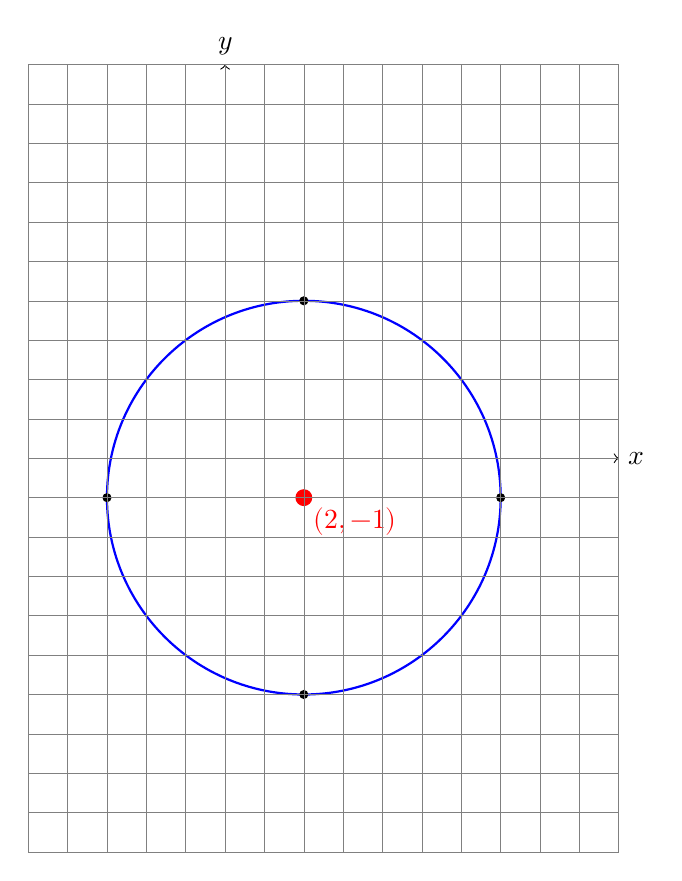
\begin{tikzpicture}[scale=0.5]
    % Draw axes
    \draw[->] (-5,0) -- (10,0) node[right] {$x$};
    \draw[->] (0,-10) -- (0,10) node[above] {$y$};
    
    % Draw the circle
    \draw[blue, thick] (2,-1) circle [radius=5];
    
    % Mark the center
    \filldraw[red] (2,-1) circle (0.2) node[below right] {$(2,-1)$};
    
    % Optional: mark radius points
    \filldraw[black] (2+5,-1) circle (0.1) node[below right] {};
    \filldraw[black] (2-5,-1) circle (0.1) node[below left] {};
    \filldraw[black] (2,-1+5) circle (0.1) node[above left] {};
    \filldraw[black] (2,-1-5) circle (0.1) node[below left] {};
    
    % Optional: grid
    \draw[very thin, gray] (-5,-10) grid[step=1] (10,10);
\end{tikzpicture}

\subsection{The Ellipse}

\begin{tcolorbox}[title=Problem 1, breakable]
    Sketch the graph of the following equations.
    In each case, indicate the center of the ellipse,
    and its extremities.
    \[\frac{x^2}{16} + \frac{y^2}{4} = 1\]
\end{tcolorbox}

\textbf{Solution:} Center is $(0, 0)$.
Extremities are $(\pm 4, 0)$ and $(0, \pm 2)$.
\begin{figure}[h!]
    \centering
    \includegraphics[width=0.5\textwidth]{images/ellipse_again.png}
\end{figure}

\subsection{The Hyperbola}

\begin{tcolorbox}[title=Problem 8, breakable]
    Sketch the graphs of the following curves, defined by the 
    given equations.

    $xy = 4$.
\end{tcolorbox}

\begin{figure}[h!]
    \centering
    \includegraphics[width=0.5\textwidth]{images/hyperbola.png}
\end{figure}

\subsection{Rotation of Hyperbolas}

\begin{tcolorbox}[title=Problem 2, breakable]
    Rotate the hyperbola $H$ defined by the equation $xy = 1$
    by $-\pi/4$. What is the equation satisfied by the image of $H$.
\end{tcolorbox}
\[v^2 - u^2 = 2\]

\begin{tcolorbox}[title=Problem 8, breakable]
    Prove the statement made in the text: If $G$ is rotation 
        and $F_r$ is a dilation by $r$, $G \circ F = F \circ G$.
\end{tcolorbox}

\begin{proof}
    Let $P = (x, y)$ be an arbitrary point.
    A dilation by $r$ is
    \[
    F_r(P) = r \begin{bmatrix} x \\ y \end{bmatrix},
    \]
    and a rotation by angle $\theta$ is 
    \[
    G(P) = \begin{bmatrix} \cos\theta & -\sin\theta \\ \sin\theta & \cos\theta \end{bmatrix} \begin{bmatrix} x \\ y \end{bmatrix}.
    \]
    Then
    \[
    G(F_r(P)) 
    = \begin{bmatrix} \cos\theta & -\sin\theta \\ \sin\theta & \cos\theta \end{bmatrix} \left( r \begin{bmatrix} x \\ y \end{bmatrix} \right)
    = r \begin{bmatrix} \cos\theta & -\sin\theta \\ \sin\theta & \cos\theta \end{bmatrix} \begin{bmatrix} x \\ y \end{bmatrix}.
    \]
    Similarly,
    \[
    F_r(G(P)) 
    = r \left( \begin{bmatrix} \cos\theta & -\sin\theta \\ \sin\theta & \cos\theta \end{bmatrix} \begin{bmatrix} x \\ y \end{bmatrix} \right)
    = r \begin{bmatrix} \cos\theta & -\sin\theta \\ \sin\theta & \cos\theta \end{bmatrix} \begin{bmatrix} x \\ y \end{bmatrix}.
    \]
\end{proof}

\end{document}
